\documentclass[12pt]{article}
\usepackage[utf8]{inputenc}
%\usepackage{nips_2017}
\usepackage{graphicx}
\usepackage{natbib}
\usepackage{booktabs}
\usepackage{float}
\usepackage{amsmath}
\usepackage{psfrag}
\usepackage{epsf}
\usepackage{enumerate}
\usepackage{centernot}

%\bibliographystyle{apalike}

%\bibliographystyle{unsrt} % Use for unsorted references 
\newcommand{\blind}{0}

%\bibliographystyle{plainnat} % use this to have URLs listed in References

% DON'T change margins - should be 1 inch all around.
\addtolength{\oddsidemargin}{-.5in}%
\addtolength{\evensidemargin}{-.5in}%
\addtolength{\textwidth}{1in}%
\addtolength{\textheight}{1.3in}%
\addtolength{\topmargin}{-.8in}%

% Title Page

\bibliographystyle{natbib}

\def\spacingset#1{\renewcommand{\baselinestretch}%
{#1}\small\normalsize} \spacingset{1}

%%%%%%%%%%%%%%%%%%%%%%%%%%%%%%%%%%%%%%%%%%%%%%%%%%%%%%%%%%%%%%%%%%%%%%%%%%%%%%

\begin{document}

\if0\blind
{
  \title{\bf The Effect of Medicaid Expansion on Non-Elderly Adult Uninsurance Rates Among States that did not Expand Medicaid}
  \author{Max Rubinstein \hspace{.2cm}\\
    and \\
    Amelia Haviland \\ \\
    Heinz College and the Department of Statistics and Data Science \\ Carnegie Mellon University}
  \maketitle
} \fi

\if1\blind
{
  \bigskip
  \bigskip
  \bigskip
  \begin{center}
  \title{\bf The Effect of Medicaid Expansion on Non-Elderly Adult Uninsurance Rates Among States that did not Expand Medicaid}
\end{center}
  \medskip
} \fi

\bigskip

\begin{abstract}

We estimate the effect of Medicaid expansion on the adult uninsurance rate in states that did not expand Medicaid in 2014 using a novel extension of the synthetic controls approach (\cite{abadie2010synthetic}). The existing literature primarily estimates treatment effects on states that expanded Medicaid. We hypothesize these effects differ: prior to the 2014 expansion, evidence suggested that Medicaid take-up rates are lower among conservative states (\cite{sommers2012understanding}), and Republicans were more likely to govern non-expansion states. We therefore hypothesize that the treatment effect on states that did not expand Medicaid would have been closer to zero than for states that did expand Medicaid. Using data from the American Communities Survey (ACS), we estimate the effect on non-expansion states by re-weighting expansion regions to approximately balance the covariates from non-expansion regions. We contribute to the literature on balancing weights by accounting for hierarchical data and measurement error in the covariates when calculating the weights. We estimate that Medicaid expansion would have changed the uninsurance rate by -2.00 percentage points (-3.59, -0.40). These results are smaller in absolute magnitude than existing estimates of the ETT (see, eg, \cite{courtemanche2017early}). We provide evidence that factors associated with Republican governance may drive this difference.

\end{abstract}

\noindent%
{\it Keywords:} Balancing weights, synthetic controls, measurement error, regression calibration, treatment effect on the controls, Medicaid expansion, uninsurance rates
\vfill

\newpage
\spacingset{1.45} % DON'T change the spacing!

\maketitle

\section{Introduction}

The 2010 Affordable Care Act (ACA) required states to expand their Medicaid eligibility requirements by 2014 to offer coverage to all adults with incomes at or below 138 percent of the federal poverty level (FPL). The United States Supreme Court ruled this requirement unconstitutional in 2012, allowing states to decide whether to expand Medicaid coverage. In 2014, twenty-six states and the District of Columbia expanded their Medicaid programs. From 2015 through 2019 an additional ten states elected to expand their Medicaid programs (\cite{KFF}). This first wave of expansions in 2014 enabled researchers to examine the effects of Medicaid expansion by using expansion states as ``treated'' states, and non-expansion states as ``control'' states. Our primary goal in this paper is to estimate the effect of 2014 Medicaid expansion on non-elderly adult uninsurance rates among states that did not expand Medicaid.

We predict that the treatment effect on non-expansion effect will be smaller in absolute magnitude than in states that expanded Medicaid in 2014. Medicaid take-up rates are lower than 100 percent and historically have varied across states. This variation is partly a function of state discretion in administering programs: for example, program outreach, citizenship verification policies, and application processes differ across states (\cite{courtemanche2017early}). Here we consider how political composition may have driven differences in take-up rates between states. Prior to the 2014 Medicaid expansion, \cite{sommers2012understanding} found that conservative political ideology was associated with lower Medicaid enrollment rates, even after controlling for a variety of other policies. Most importantly, political ideology appears to have largely driven a state's decision to expand Medicaid in 2014. Figure~\ref{fig:stateideology} plots a measure of each state's 2013 institutional ideology by their Medicaid expansion status (\cite{fording}). Higher values of this score correspond to more liberal government institutions. The red dashed line indicates the mean expansion state score and the gray dashed line indicates the mean non-expansion state score. Figure~\ref{fig:stateideology} illustrates that non-expansion states are more conservative than expansion states. If the differential take-up rates observed by \cite{sommers2012understanding} continue to hold post-expansion, we should expect treatment effects on non-expansion states to be smaller in absolute magnitude than treatment effects on expansion states. 

\begin{figure}
    \begin{center}
    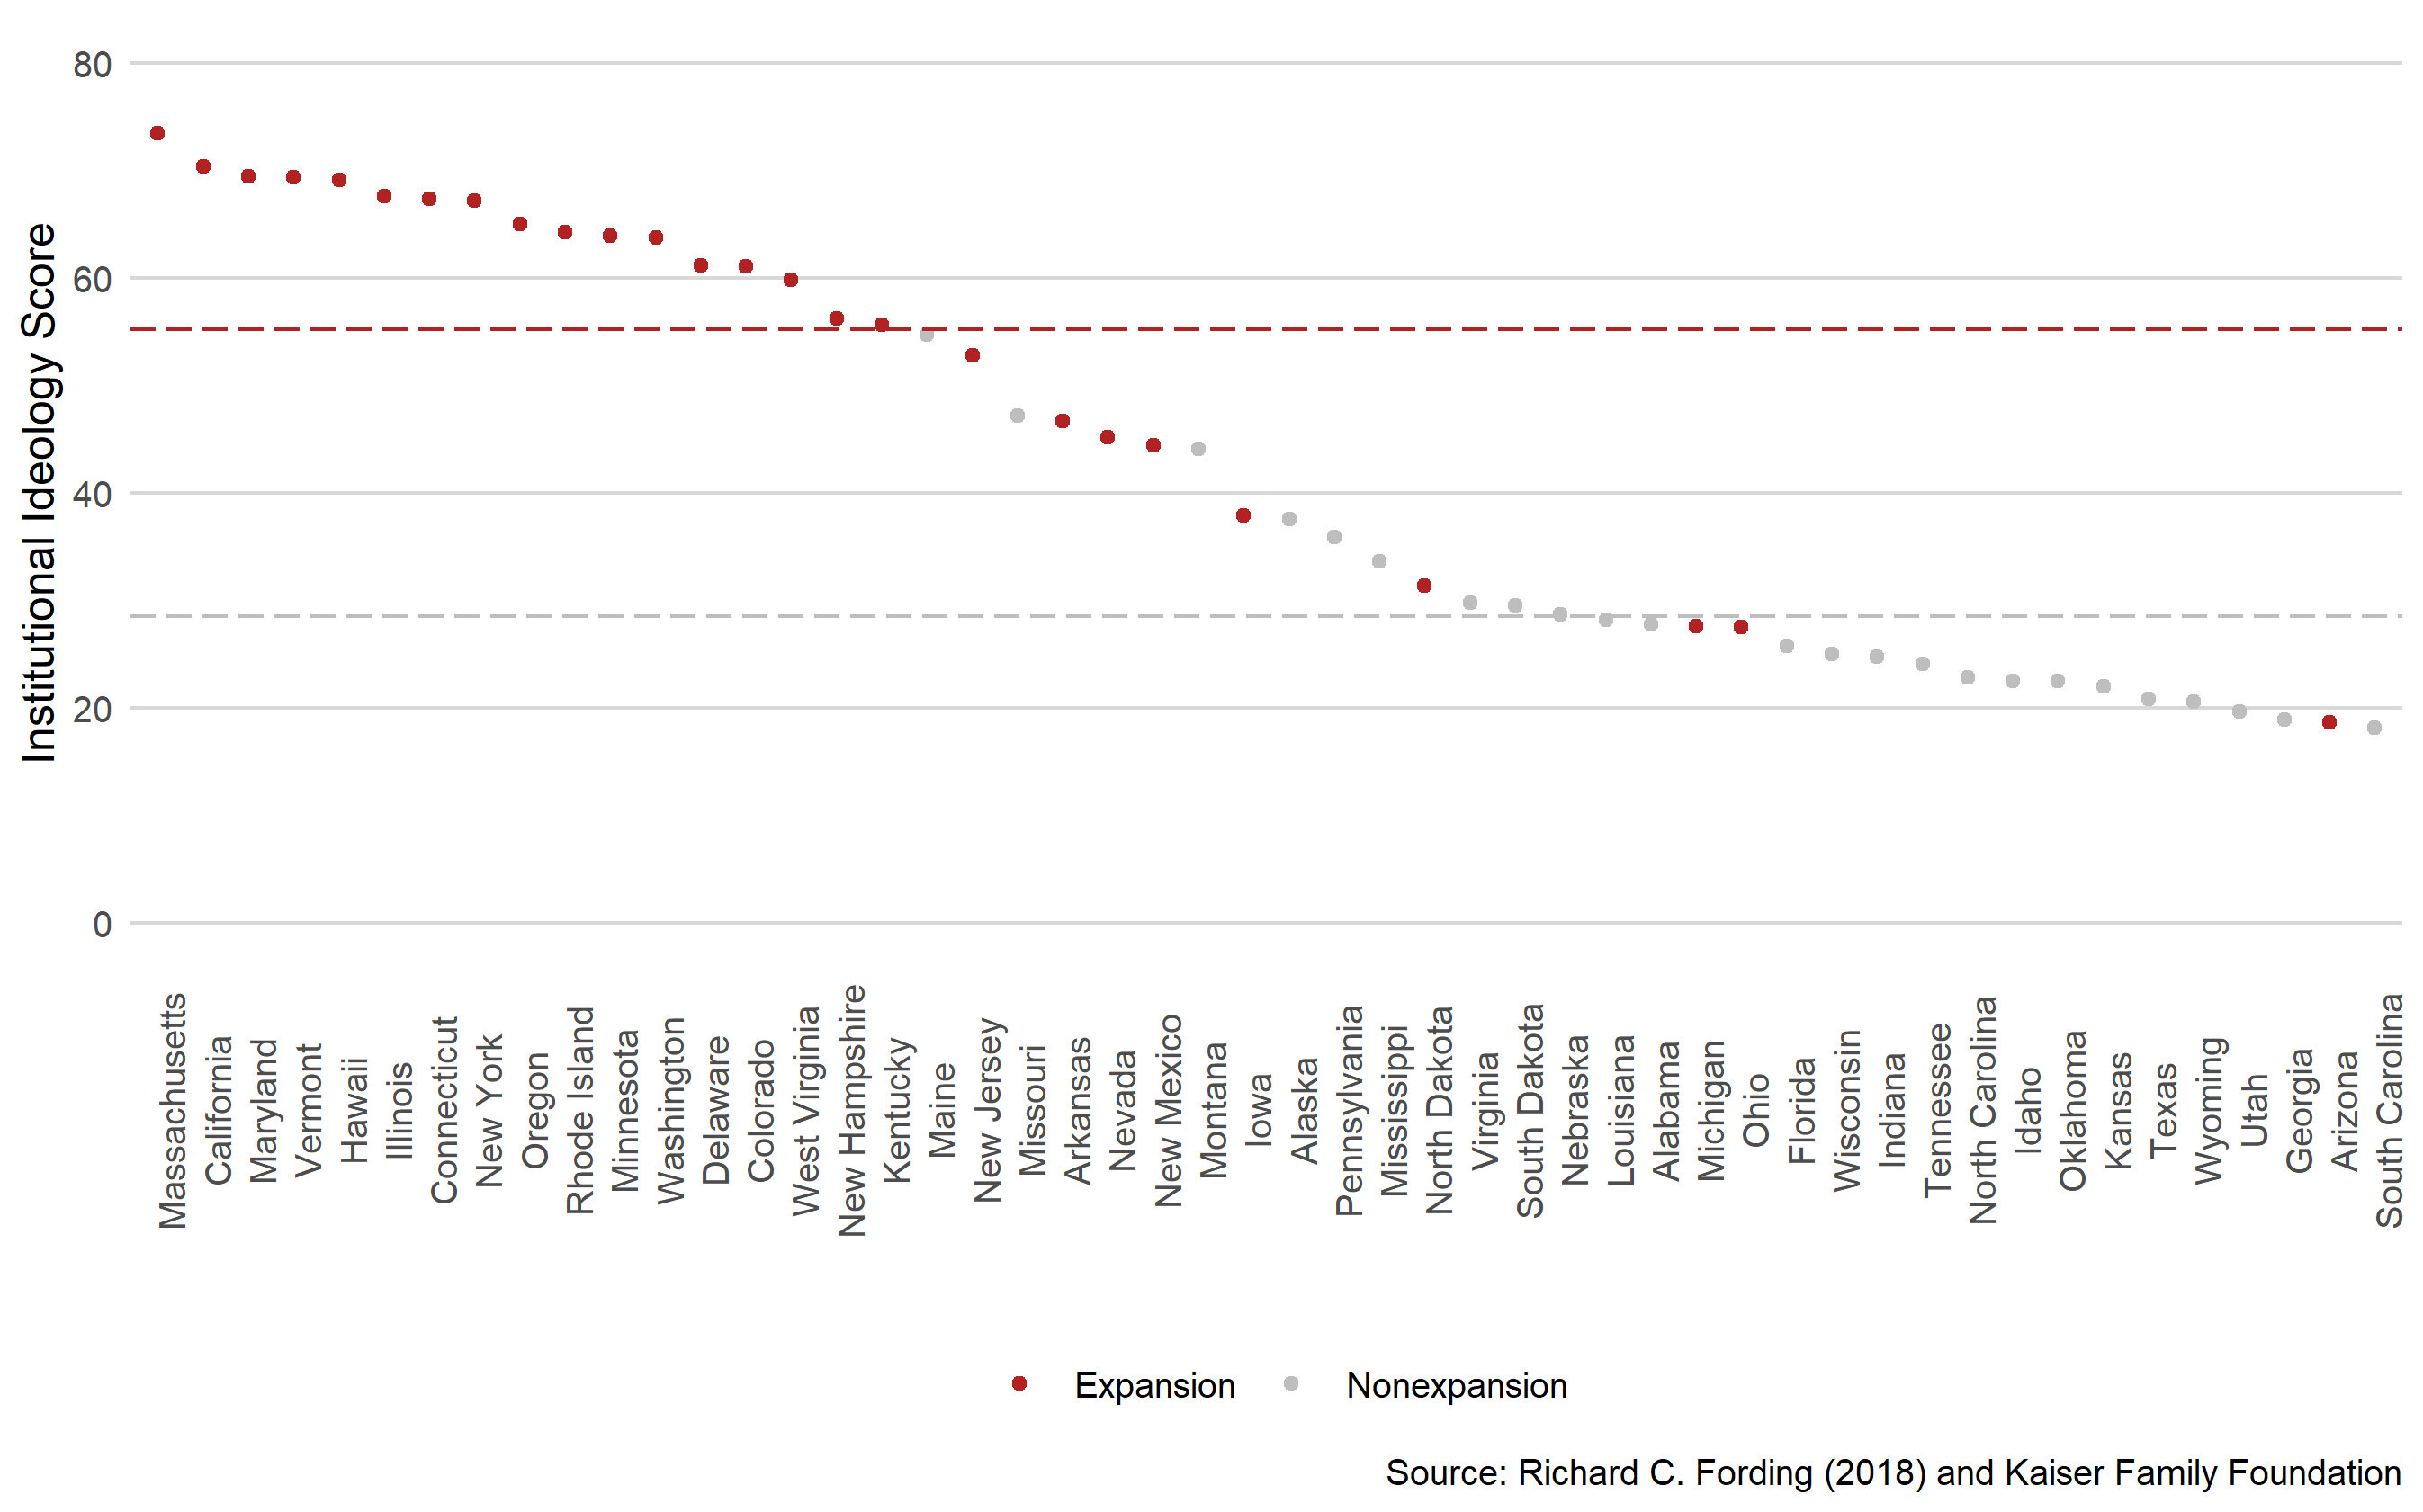
\includegraphics[scale=0.7]{01_Plots/political-expansion-plot.png}
    \caption{Government ideology and Medicaid expansion}
    \label{fig:stateideology}
    \end{center}
\end{figure}

This paper makes two methodological contributions to the literature on balancing weights. First, we extend the ``synthetic controls'' framework to estimate the treatment effect on the controls (ETC) using longitudinal data and we clarify the required assumptions. In brief, while balancing on pre-treatment outcomes alone arguably suffices for some synthetic control applications (see, eg, \cite{botosaru2017role}), because our goal in this setting is to estimate treatment response, we must therefore balance on all covariates that predict treatment response, not just the outcome level absent treatment. Moreover, we cannot simply leverage pre-treatment data to conduct variable selection in this setting. We instead use an implementation of Stable Balancing Weights (\cite{zubizarreta2015stable}) to estimate a set of positive weights to weight the expansion regions to approximately match the covariate distribution of the non-expansion regions. 

Our second contribution is to modify the Stable Balancing Weights (SBW) objective function to account for our data, which is both hierarchical and has several covariates measured with error. Specifically, we use data from the American Communities Survey (ACS) aggregated to the consistent public use microdata area (CPUMA) level. These regions nest within states, and using these smaller regions allows us to get better covariate balance. However, as a result our data both has a hierarchical structure (regions within states) and, because our region-level covariates are estimated from underlying survey data, the sampling variability from our covariate estimates is a form of measurement error which may bias our treatment effect estimates. We first propose a modification of the SBW criterion to account for the hierarchical nature of the data, which disperses the weights more evenly across states. We then leverage the replicate survey weights provided in the ACS microdata to estimate the covariance matrix associated with the sampling variability and use this information to correct for this bias, following the regression calibration literature (see, eg, \cite{gleser1992importance}). This is the first study we are aware of that attempts to adjust for hierarchical data structure and measurement error in the covariates when using balancing weights. 

The remainder of this paper has the following structure. Section II provides an overview of the data and defines the study period, outcome, covariates, and treatment. Section III discusses our methods, beginning by defining our target estimand, and then outlining our identification, estimation, and inferential procedures. Section IV presents our primary results and sensitivity analyses. Section V provides a brief discussion of the policy relevance of our findings, and Section VI contains a brief concluding summary of the paper. Supplemental materials may be found in the Appendices.

\section{Data}

Our primary data source is the annual household and person public use microdata files from the American Community Survey (ACS) from 2011 through 2014. The ACS is an annual survey of approximately three million individuals across the United States. The public use microdata files include information on individuals in geographic areas greater than 65,000 people. The smallest geographic unit contained in these data are public-use microdata areas (PUMAs), arbitrary boundaries that nest within states but not within counties or other more commonly used geographic units. One limitation of these data is a 2012 change in the PUMA boundaries, which do not overlap well with the previous boundaries. As a result, the smallest possible geographic areas that nest both PUMA coding systems are known as consistent PUMAs (CPUMAs). The United States contain 1,075 total CPUMAs, with states ranging from having one CPUMA (South Dakota, Montana, and Idaho) to 123 CPUMAs (New York). The average total number of sampled individuals per CPUMA across the four years within our primary dataset of 929 CPUMAs (discussed in Section \ref{sssec:txassign}) is 1,001; the minimum number of people sampled was 334 and the maximum is 23,990. Importantly, this survey does not follow specific individuals over time but rather reflects a different sample of individuals each year.

\subsection{Study period}

We begin our analysis in 2011 following \cite{courtemanche2017early}, who note that several other aspects of the ACA were implemented in 2010 -- including the provision allowing for dependent coverage until age 26, and the elimination of co-payments for preventative care -- and likely induced differential shocks across states. We also restrict our post-treatment period to 2014: several additional states expanded Medicaid in 2015, including Indiana, Michigan, and Pennsylvania. However, these states did not expand Medicaid contemporaneously with the 2014 ACA provisions. Without additional assumptions, this second-year expansion cannot help us estimate the effect of the 2014 expansion. 

\subsection{Covariates}

We use the underlying individual-level ACS survey data and accompanying survey weights to aggregate the data at the CPUMA level. We choose our covariates to approximately align with those considered in \cite{courtemanche2017early} and that are likely to be potential confounders. Because we are ultimately interested in calculating rates, these variables include both the numerator and denominator counts.\footnote{When viewing the denominator variables as random, these ratio estimators will in general be biased; however, this bias decreases quickly with the sample size (is $O(n^{-1})$); given that our CPUMA sample sizes are all over 300 we treat these estimates as unbiased in our analysis.}

Using the ACS survey weights, we first estimate: the total non-elderly adult population for each year 2011-2014; the total labor force population (among non-elderly adults) for each year 2011-2013; and the total number of households averaged from 2011-2013. We also construct an average of the total non-elderly adult population from 2011-2013. These are our denominator variables. For our numerator counts, we estimate the total number of: females; whites; people of Hispanic ethnicity; people born outside of the United States; citizens; people with disabilities; married individuals; people with less than high school education, high school degrees, some college, or college graduates or higher; people living under 138 percent of the FPL, between 139 and 299 percent, 300 and 499 percent, more than 500 percent, and who did not respond to the income survey question; people aged 19-29, 30-39, 40-49, 50-64; households with one, two, or three or more children, and households that did not respond about the number of children.\footnote{Number of children and income to poverty ratio were the only two variables with missing data in the underlying microdata.} We average these estimated counts using the ACS survey weights from 2011-2013. For each individual year from 2011-2013, we estimate the total number of people who were unemployed and uninsured at the time of the survey (calculated among all non-elderly adults and all non-elderly adults within the labor force, respectively). We divide the numerator counts by the corresponding denominator counts to estimate the percentage in each category. For the demographics, these include the average number of non-elderly adults from 2011-2013. For the time-varying variables, we use the corresponding year (where uninsurance rates are calculated as a fraction of the labor force rather than the non-elderly adult population). We also calculate the 2011-2012 and 2012-2013 non-elderly adult population growth, and the average number of households to adults across 2011-2013. 

In addition to the ACS microdata, we use Census data to calculate the approximate percentage of people living within an ``urban'' area for each CPUMA (\cite{census}). Finally, we include three state-level covariates reflecting the partisan composition of each state's government in 2013. Specifically, we use data from the National Conference of State Legislatures (NCLS) to generate an indicator for states with a Republican governor, an indicator for states with Republican control over the lower legislative chamber, and an indicator for states with Republican control over both chambers of the legislature and the governorship.\footnote{Nebraska is the only state with a unicameral legislature; moreover, the legislature is technically non-partisan. We nevertheless classified them as having Republican control of the legislature.} 

\subsection{Outcome}

Our outcome of interest is the non-elderly adult uninsurance rate in 2014, which we donate using $Y$. While take-up among the Medicaid-eligible population is a more natural outcome, we choose the non-elderly adult uninsurance rate for two reasons, one theoretic and one practical. First, Medicaid eligibility in the post-period is likely endogenous: Medicaid expansion may affect an individual's income and poverty levels, which in general define Medicaid eligibility. A second reason is to align our study with others to compare our results with the existing literature, and this is the outcome that \cite{courtemanche2017early} use. One drawback of using this outcome is that the simultaneous adoption of other ACA provisions in 2014 more clearly affects this rate in a way that a more targeted group might not be.

\subsection{Treatment assignment} \label{sssec:txassign}

While some states expanded Medicaid and other states did not, assigning a binary treatment status simplifies a more complex reality. There are three reasons to be cautious about this simplification. First, states differed substantially in their Medicaid coverage policies prior to 2014: with perfect data we might consider Medicaid expansion as a continuous treatment with values proportional to the number of newly eligible individuals. The challenge though is correctly identifying newly eligible individuals in the data (see \cite{frean2017premium}, who attempt to address this). Second, \cite{frean2017premium} note that five states (California, Connecticut, Minnesota, New Jersey, and Washington) and the District of Columbia adopted partial limited Medicaid expansions prior to 2014. \footnote{\cite{kaestner2017effects} and \cite{courtemanche2017early} also consider Arizona, Colorado, Hawaii, Illinois, Iowa, Maryland, and Oregon to have had early expansions.} Lastly, timing is an issue: among the states that expanded Medicaid in 2014, Michigan's expansion did not go into effect until April 2014, while New Hampshire's expansion did not occur until September 2014.

Our primary analysis excludes New York, Vermont, Massachusetts, Delaware, and the District of Columbia from our pool of expansion regions, because these regions had comparable Medicaid coverage policies prior to 2014 (\cite{kaestner2017effects}). We also exclude New Hampshire because it did not expand Medicaid until September 2014. While Michigan expanded Medicaid in April 2014, we leave this state in our pool of treated states. We consider the remaining expansion states as ``treated'' and the non-expansion states as ``control'' states. We later consider the sensitivity of our results to these classifications by removing the early expansion states noted by \cite{frean2017premium}. Our final dataset contains aggregated statistics for all of the above variables for 925 CPUMAs in our non-expansion and our pool of expansion states. There are 414 CPUMAs among 24 non-expansion states and 515 CPUMAs among 22 expansion states. When we exclude the early expansion states for sensitivity analyses, we are left with 296 CPUMAs across 17 states.

\section{Methods}
\label{sec:methods}

In this section we present our causal estimand, identifying assumptions, estimation strategy, and inferential procedure.

\subsection{Estimand}

Our goal is to estimate the average effect 2014 Medicaid expansion would have had on the non-elderly adult uninsurance rate in states that did not expand Medicaid. Let $c$ index a CPUMA, $s$ index the state, and $t$ index the time period. Let $N_1$ be the number of treated CPUMAs, $N_0$ be the number of control CPUMAs, and $N$ be the total number of CPUMAs. Similarly, let and $M = M_1 + M_0$ states (with $M_1$ and $M_0$ defined analogously). Each state has $n_s$ CPUMAs. Since we are only interested in the counterfactual at time $T = 2014$, we simplify notation by removing this variable and the subscript and write our formal estimand as:

$$
\psi = \psi^1 - \psi^0 = N_0^{-1}\sum_{s, c: A_s = 0} Y_{sc}^{A_s = 1} - Y_{sc}^{A_s = 0}
$$

We observe $\psi^0$ in the data; the challenge is estimating $\psi^1$ using our pool of treated units. That is, we wish to predict the counterfactual uninsurance rates in 2014 for states that did not expand Medicaid expansion had they expanded their Medicaid eligibility requirements. \foonote{The 2014 Medicaid expansion occurred simultaneously with the implementation of several other major ACA provisions, including (but not limited to) the creation of the ACA-marketplace exchanges, the individual mandate, health insurance subsidies, and community-rating and guaranteed issue of insurance plans (\cite{courtemanche2017early}). Almost all states broadly implemented these reforms beginning January 2014. Conceptually we think of the other ACA components as a state-level treatment ($V$) separate from Medicaid expansion ($A$). Therefore, our total estimated effect may also include interactions between these policy changes; however, we do not attempt to separately identify these effects. Because the ACA implementation and Medicaid expansion may vary over time, we do not try to generalize these results beyond 2014.} 

\subsection{Identification}

The following causal assumptions are necessary (though not sufficient) to enable us to identify our target parameter from the data: consistency, no unmeasured confounding, no anticipatory treatment effects, and positivity of treatment assignment. We explain these assumptions in detail and their consequences below. We additionally invoke several parametric assumptions to help us identify our causal parameter given the measurement error in our covariates.

Consistency states that the observed factual outcome under a given treatment assignment is equal to the potential outcome under that same treatment assignment ($Y_{sc}^{A_{sc} = a} = Y_{sc} \mid A_{sc} = a$). In other words, we assume that one regions' treatment assignment does not affect another regions' observed outcome. This is a standard assumption, but is often not realistic. Violations of this assumption are likely in our setting: for example, \cite{frean2017premium} find evidence that Medicaid expansion drove previously eligible but uninsured individuals to enroll in Medicaid in both expansion and non-expansion states. Signing the potential bias from this violation requires redefining the causal estimand: for example, we might consider the treatment effect on the untreated given that all states have expanded Medicaid, where the contrast is against where only the observed expansion states expanded Medicaid. If spillovers occurred in equal proportions across each region, and the magnitude of the spillovers increase with the total number of treated regions, then the true effect would be larger in absolute magnitude than the estimated estimated using the observed data. We could consider other estimands or assumptions to get different predictions about the sign of the bias; however, this is beyond the scope of this paper.

We next assume that there were no anticipatory treatment effects. Letting treatment occur at time $T$, we have that for $t < T$:

$$
Y_{sct} = Y_{sct}^0
$$

This assumption is necessary because we are conditioning on pre-treatment outcomes. If these outcomes were affected by the treatment before it were implemented, these covariates would be endogenous. Anticipatory treatment effects may occur if plans to expand Medicaid induce uninsured but Medicaid-eligible individuals to enroll in Medicaid prior to expansion. We do not think these violations occurred in large enough numbers to substantially affect our results. Instead, we address a more concerning version of this violation: the fact that several states allowed certain counties to expand Medicaid prior to 2014. We therefore test the sensitivity of our results to the exclusion of these states.

Third, we assume no unmeasured confounding; that is, that at time $T$ the potential outcomes for each CPUMA are independent of the state-level treatment assignment conditional on the population-level CPUMA and state-level covariates $X_{sc}$ (which includes pre-treatment outcomes):

$$
Y_{sc}^a \perp A_{sc} \mid X_{sc}
$$

While unverifiable, we believe it is reasonable here given our rich covariate set. To be explicit, we believe that the potential uninsurance rates for each CPUMA are independent of the treatment assignment conditional on the percentage of uninsured individuals in each year of the pre-treatment period, the percentage of unemployed individuals in each year of the pre-treatment period, the population growth in 2012 and 2013, the average ratio of households to non-elderly adult population, the state's political composition, the average proportion of households with one, two, or three or more children during the pre-treatment period, the average proportion of households who did not respond about their number children, and the average proportion of individuals during the pre-treatment period with given demographics noted above (age group, sex, white, Hispanic ethnicity, US citizenship, foreign born, income-to-poverty group (including non-response), disability status, urban residence, and educational attainment group). 

Finally, we assume positivity of treatment assignment; that is, that all states had some non-zero probability of being treated $\pi(X_{1s}, ..., X_{n_ss}) > 0$. Positivity violations can cause a lack of covariate overlap in the observed data. Overlap is an issue in this study. We address this in multiple ways that we outline in our estimation strategy below. 

These assumptions are sufficient to non-parametrically identify our causal estimand if we observed the true covariates $X_{sc}$. Unfortunately, for our covariates estimated using the ACS data, we do not observe the true values of $X_{sc}$ but rather a mean-unbiased estimate $W_{sc}$. Importantly, $Y_{sc}^a \perp A_{sc} \mid X_{sc} \centernot\implies Y_{sc}^a \perp A_{sc} \mid W_{sc}$. The use of these proxies may also bias our estimates; we therefore rely on several modeling assumptions to correct for this bias.

First, we assume that the potential outcome under treatment is linear in the covariates $X_{sc}$. Specifically, we assume that the following model generates the potential non-elderly adult uninsurance rate under treatment:

$$
Y_{sc}^1 = \alpha + X_{sc}^T\beta + \epsilon_{sc} + c_s
$$

We assume that the errors $\epsilon_{sc}$ and $c_s$ are independent from each other and across time (ie we rule out serial-correlation), and that these errors are invariant to the intervention. This model then allows us to identify $\psi^1$ in terms of our model parameters; specifically, we have that $\psi^1 = \alpha + \bar{X}_0^T\beta$, where $\bar{X}_0$ is the (observed) mean covariate values among the control units.\footnote{To be precise, we use the population-weighted mean so as to target the individual-level treatment effect rather than the CPUMA-average treatment effect.} 

A classical assumption in the measurement-error literature is that $X$ and $W$ are jointly normally distributed, the measurement errors are independent and identically distributed, and these errors are uncorrelated with the outcome. Under these assumptions, it is well-known that standard regression-based estimates of $\beta$ will suffer from the following bias:

$$
\mathbb{E}\{\hat{\beta}\} = \kappa \beta
$$

where $\kappa = \Sigma_{WW \mid A = a}^{-1}\Sigma_{XX \mid A = a}$. Our causal parameter is a function of $\beta$, which is estimable from the data if we know (or can estimate) $\kappa$ (\cite{gleser1992importance}). 

Under the classical errors-in-variables model, the asymptotic bias for the SBW estimator that sets $\delta = 0$ is equivalent to the bias of a linear combination of coefficient estimates from the OLS-based regression estimator. The intuition for this result is as follows: exact balancing weights estimate an implicit $\beta$ on a subset of the data where we have sufficient overlap. We can therefore think of SBW as returning a solution to some implicit weighted-least squares problem. If we assume that the outcome model holds across all of the data, WLS and OLS are estimating the same $\beta$; therefore, the bias that effects the least squares solution will have the same effect on the WLS, and therefore SBW, solution. Our target parameter is therefore identified under the same conditions regardless of the estimation strategy. We prove this result more formally in Appendix A.

For this application we make a slight departure from the classical setting, assuming that that $W_{sc} = X_{sc} + v_{sc}$, where $\sqrt{s_{sc}}v_{sc}$ are drawn iid from $MVN(0, \Sigma_{vv \mid A = a})$, and where $s_{sc}$ are the vector of sample sizes used to calculate $W_{sc}$. We again assume that $v_{sc}$ is independent of the CPUMA-level errors $\epsilon_{sc}$ (which may include measurement error in the outcome) and the state-level errors $c_s$. We believe this is reasonable because the errors in the CPUMA-level aggregates are estimated from a 2014 cross-section of individuals, while the covariates are estimated from different individuals surveyed from 2011-2013. \footnote{While the sample sizes for each CPUMA are all relatively large, the variance is still larger than one might expect due to the design effect of the survey.} 

\subsection{Estimation}

We outline our estimation strategy first emphasizing how our method differs from the synthetic controls approach, which motivates our use of the SBW objective. Second, we explain a modification we make to the SBW criterion to address the hierarchical data structure (which we call H-SBW) that reduces the variance of our estimator under our assumption of within-state correlation of our model errors. Third, we connect our estimator to the regression calibration literature by generating weights that balance a linear prediction of the true covariates $\hat{\eta}_a(W_{sc})$ using the observed covariates $W_{sc}$. 

We also test the sensitivity of our estimator to a ridge-augmented version, following the suggestion of \cite{ben2018augmented}; this allows us to achieve better covariate balance by extrapolating beyond the support of the data. As a separate sensitivity check, we estimate a different causal parameter -- the overlap average treatment effect (OATE) -- using overlap weights, as discussed in \cite{li2018balancing}. Estimating this effect does not require extrapolation, but rather changing the target estimand. We discuss this further below.

Similar to synthetic controls applications, we seek to generate a set of positive weights that balance the means of covariates for the treated units to the mean of covariates for the control units. Assume that we observe the true covariate matrices $X_1$ and $X_0$, and let $\bar{X}_0$ be the (population-weighted) average of the covariate values in the non-expansion region. Ideally, we could then find some $\gamma^\star$ such that for $\delta = 0$: 

$$
(\frac{1}{N_0}X_1^T\gamma^\star - \bar{X}_0) \le \delta, \gamma_i^\star > 0, \sum_{sc} \gamma_{sc}^\star = N_0
$$

Let $p$ be a vector of (normalized) population weights for each CPUMA in the non-expansion region in year $T = 2014$. We could then estimate $\psi$ as

$$
\hat{\psi} = (N_0^{-1}\sum_{s: A_s = 1}^{M_1}\sum_{c = 1}^{n_s}\gamma_{sc}^\star Y_{sc} - \sum_{s: A_s = 0}\sum_{c = 1}^{n_s}Y_{sc}p_{sc})
$$

The assumption that the outcomes (absent treatment) follow a linear factor model frequently motivates the synthetic controls approach; here we instead assume no unobserved confounding and assume that the outcomes given treatment $\mu_1(X_{sc}) = \alpha + X_{sc}^T\beta$. The bias of our estimator (again assuming we observed $X_{sc}$), is therefore less than or equal to $\lvert\beta\rvert^T\delta = 0$ (see, eg, \cite{zubizarreta2015stable}). The challenge, however, is that for any given dataset we have no guarantee that any such $\gamma$ exists that exactly balances the covariates; we therefore need some method of determining how to prioritize which parts of the covariate distribution we wish to balance to minimize this bias.

This is where estimating the ETC contrasts with the commonly used synthetic control approach used to estimate the ETT: \cite{abadie2010synthetic} determine how to prioritize covariate balance by training their model on pre-treatment outcomes (\cite{kaul2015synthetic} shows that often the most relevant covariates simply become the pre-treatment outcomes). Because in that setting $Y^0_{sct}$ is actually observed for $t \le T_0$, \cite{abadie2010synthetic} are able to leverage this data to select the covariates that best predict these values. By contrast we never observe $Y^1_{sct}$ prior to treatment. Without additional assumptions, we cannot use the pre-treatment data to learn which covariates matter most for determining this potential outcome.

Moreover, the problem of predicting treatment response also makes estimating the ETC more challenging to estimate than the ETT. In particular, we likely care more about balancing ``auxillary covariates'' (covariates that are not pre-treatment outcomes) in our setting than the traditional synthetic controls setting. To see this, assume that both $\mu_0$ and $\mu_1$ are linear in the covariates, including the pre-treatment outcomes. We might reasonably believe the coefficients on the auxillary covariates are close to zero once we condition on pre-treatment outcomes. As a result, the bias induced by remaining imbalances on the auxillary covariates would be small. On the other hand, the coefficients on the same covariates for the model $\mu_1(X_{sc})$ could be much larger, even after conditioning on pre-treatment outcomes, because these coefficients are highly predictive of treatment response. If our weights fail to balance these covariates, we should expect that our estimates of $\mu_0$ will in general have less bias than our estimates of $\mu_1$. In summary, estimating the ETC requires a greater understanding of how the covariates are related to treatment response than the ETT; moreover, we cannot learn this information by using pre-treatment outcomes.

We therefore estimate the ETC by using a variation of SBW that we call H-SBW.\footnote{Specifically, we use a modified implementation of Noah Griefer's ``optweight'' package in R, available on github.com/mrubinst757}. This procedure allows us to estimate the minimum variance weights that satisfy user-specified balance constraints. Let $\eta_a(W_{sc}) = \mathbb{E}\{X_{sc} \mid W_{sc}, A_s = a\}$, and $\hat{\eta}_1(W_1)$ be a matrix of estimates of $\eta_1(W_1)$. Let $\bar{W}_0$ be a vector of population-weighted estimates of the covariates for the non-expansion region.\footnote{Because $\bar{W}_0$ and $\bar{X}_0$ are equal in expectation, the use of this target will not contribute to any asymptotic bias of our estimator.} We generate weights that solve the following objective:

$$
\min_{\gamma \in \Gamma} \sum_{s: A_s = 1}^{M_1}(\sum_{c = 1}^{n_s} \gamma_{sc}^2 + \sum_{c \ne d}\rho \gamma_{sc}\gamma_{sd})
$$

$$
\Gamma := \{\gamma \mid \frac{1}{N_0}\hat{\eta}_1(W_{sc})^T\gamma - \bar{W}_0 \mid \le \delta, \gamma_{sc} > 0, \sum_{sc}\gamma_{s,c} = N_0\}
$$

This objective is a modification of the SBW objective, which sets $\rho = 0$ and balances on $W_{sc}$ rather than $\eta_1(W_{sc})$. Importantly, both allow the user to specify covariate-level balance constraints using the vector $\delta$. When estimating the ETC, we lean heavily on assumptions to justify our choice of $\delta$; in particular, we use a priori domain knowledge about which covariates are most likely to be important predictors of treatment effect heterogeneity when setting $\delta$. However, we also must choose $\delta$ to something that is feasible given the data. 

For our application, we constrain $\delta$ to be 0.05 percentage points for pre-treatment outcomes, 0.1 percentage points for pre-treatment uninsurance rates. We believe these are the most likely factors associated with treatment response, so we prioritize balancing these covariates. For the remaining covariates, we let $\delta$ be 0.25 percentage points for population growth, 1 percentage point for female, hispanic ethnicity, white race, age category, disability, and number of children category; 2 for urban, citizenship, education category, income-to-poverty category, student, and foreign-born; and 20 for the Republican governance indicators. We choose these constraints primarily on feasibility concerns, and for our variance estimates, we programmatically reduce these initial constraints when this constraint set becomes infeasible.

We now discuss how H-SBW differs from SBW, beginning with the criterion. The motivation of the SBW criterion, which is equivalent to ours with $\rho = 0$, is to produce the minimum variance weights for a fixed $\delta$. This is optimal if, for example, the errors in the outcome model are independent and identically distributed. In our setting we have possible state-level dependencies, reducing the efficiency of this estimator. To improve the efficiency, we add the tuning parameter $\rho$, which attempts to more uniformally disperse the weights across states. This objective is optimal if we assume constant within-state correlation of the errors and constant variance across units. We discuss this objective in more detail and provide simulation results in Rubinstein (2021) (pre-print available soon); broadly speaking, we can think of H-SBW being to SBW what generalized least squares (GLS) is to ordinary least squares (OLS): both SBW and OLS can produce unbiased estimates of model parameters; however, H-SBW and GLS can be produce efficient estimators assuming a block-matrix correlation structure in the outcome errors. 

A second departure from SBW comes in the constraint set: rather than balancing on the observed covariate values $W_{sc}$, we instead balance on our estimate of $\eta_1(W_{sc})$. This is because the estimation error in these CPUMA-level covariates will bias our estimate of $\psi^1$. In Appendix A we show that if we had access to $\eta_1$, we could obtain an unbiased estimate of the super-population parameter $\psi^1 = \mathbb{E}\{Y_i^1 \mid A_i = 0\}$ by balancing on $\eta_1(W_{sc})$.\footnote{For the finite-sample parameter we're interested in here, using the conditional expectation still leads to some finite-sample bias.} Of course, in practice we do not know $\eta_1$ but must estimate it using auxillary data. Here we leverage the person-level replicate survey weights provided in the ACS microdata to estimate the variability in each CPUMA's observed covariate values. We then use a variant of regression calibration techniques to estimate $\eta_a(W_{sc})$ as a linear approximation to the true covariate values (see, eg, \cite{gleser1992importance}, \cite{carroll2006measurement}). We consider two versions of this procedure: our preferred version which accounts for the fact that some covariates are estimated much more precisely than others, but that assumes that all of the differences in the errors are attributable to the different sample sizes used to estimate the covariates; and a second that follows the traditionally used procedures in this setting which does not account for this differential precision, but does not model the differential sampling variability, and instead averages over all observed variance estimates. Further details about these covariate adjustment procedures are available in Appendix B.

This is the first application we are aware of to use regression calibration methods in the context of balancing weights. We emphasize two critical assumptions for using this procedure in our context: (1) the outcome model is linear in the true covariates; (2) the measurement error in the outcome is unrelated to the measurement error in the covariates. The first assumption is strong, though often used in practice. The second assumption is reasonable, because our outcomes are estimated from a different cross-section of individuals than our covariates. 

Lastly, we are unable to achieve exact balance, which will also contribute to the bias of our estimator. Following the recent literature on synthetic controls, we test the sensitivity of our results to these imabalances by using ridge-regression augmented weights \cite{ben2018augmented}. Letting $\hat{\eta}_1(W_1)$ be the matrix of adjusted covariates, and $\gamma^{hsbw}$ be our H-SBW weights, we standardize our weights to sum to one and estimate the regression-augmented weights:

$$
\gamma^{aug} = \gamma^{hsbw} + (\hat{\eta}_1(W_1)^T\gamma^{hsbw} - \bar{W}_0)^T(\hat{\eta}_1(W_1)^T\Omega^{-1}\hat{\eta}_1(W_1) + \lambda I_d)^{-1}\hat{\eta}_1(W_1)^T\Omega^{-1}
$$

where $\Omega$ is a block diagonal matrix with diagonal entries equal to one and the within-group off diagonals equal to $\rho$. We choose $\lambda$ so that the remaining imbalances all fall within 0.1 percentage points (see \cite{ben2018augmented} for more details on the connection between these weights and ridge-regression). The cost of this procedure is that we must extrapolate from the support of the data, and therefore rely more heavily on our modeling assumptions. In our results we consider estimators using SBW ($\rho = 0$), H-SBW ($\rho = 0.2$), and ridge-augmented versions of SBW and H-SBW that we call BC-SBW and BC-HSBW. We focus our discussion on our preferred estimator, H-SBW, and its ridge augmented version BC-HSBW. 

\subsection{Inference}

We treat our estimate of $\psi^0$ as known, since the population-weighted CPUMA average of observed values is quite precisely estimated relative to the CPUMA-level averages. We also treat our balancing targets $\bar{W}_0$ as known for the same reason. 

We then evaluate the uncertainty in our estimator with respect to our model-based estimates of $\psi^1$. We then use the leave-one-state-out jackknife to estimate the standard error of our estimator of $\psi^1$ (\cite{cameron2015practitioner}). Our preferred estimators conditions on our estimates of $\eta_1(W_{sc})$; however, we also calculate a second estimate that recalculates the entire adjustment process. While this latter estimator accounts for the additional uncertainty in our estimate of $\eta_1$, we expect this estimator to be overly conservative: the variability in our estimate of $\eta_1$ occurs at the CPUMA-level, but this procedure re-samples entire states to approximate this uncertainty. We therefore present the standard errors that condition on the adjustment process in the paper, and leave the results from full-procedure jackknife confidence interval results to Appendix E. 

\section{Results}

The following results use our preferred covariate adjustment $\hat{\eta}_1(W_{sc})$. Figure~\ref{fig:loveplotc1} shows how our balancing weights reduce the imbalances among covariates with greater than one percentage point difference between the targeted mean in the expansion region and the mean values in the non-expansion region (we target the population-weighted mean of the untreated region). Before applying our weights, we see that there are substantial imbalances in the Republican governance indicators, as well as pre-treatment uninsurance and unemployment rates. Our weights drastically reduce these differences; however, some imbalances remain. In particular, imbalances remain in the Republican governance indicators. A complete balance table is available in Appendix D, Table~\ref{tab:baltab1} and Table~\ref{tab:baltab2}. Appendix C contains additional summary statistics.

\begin{figure}[B]
\begin{center}
    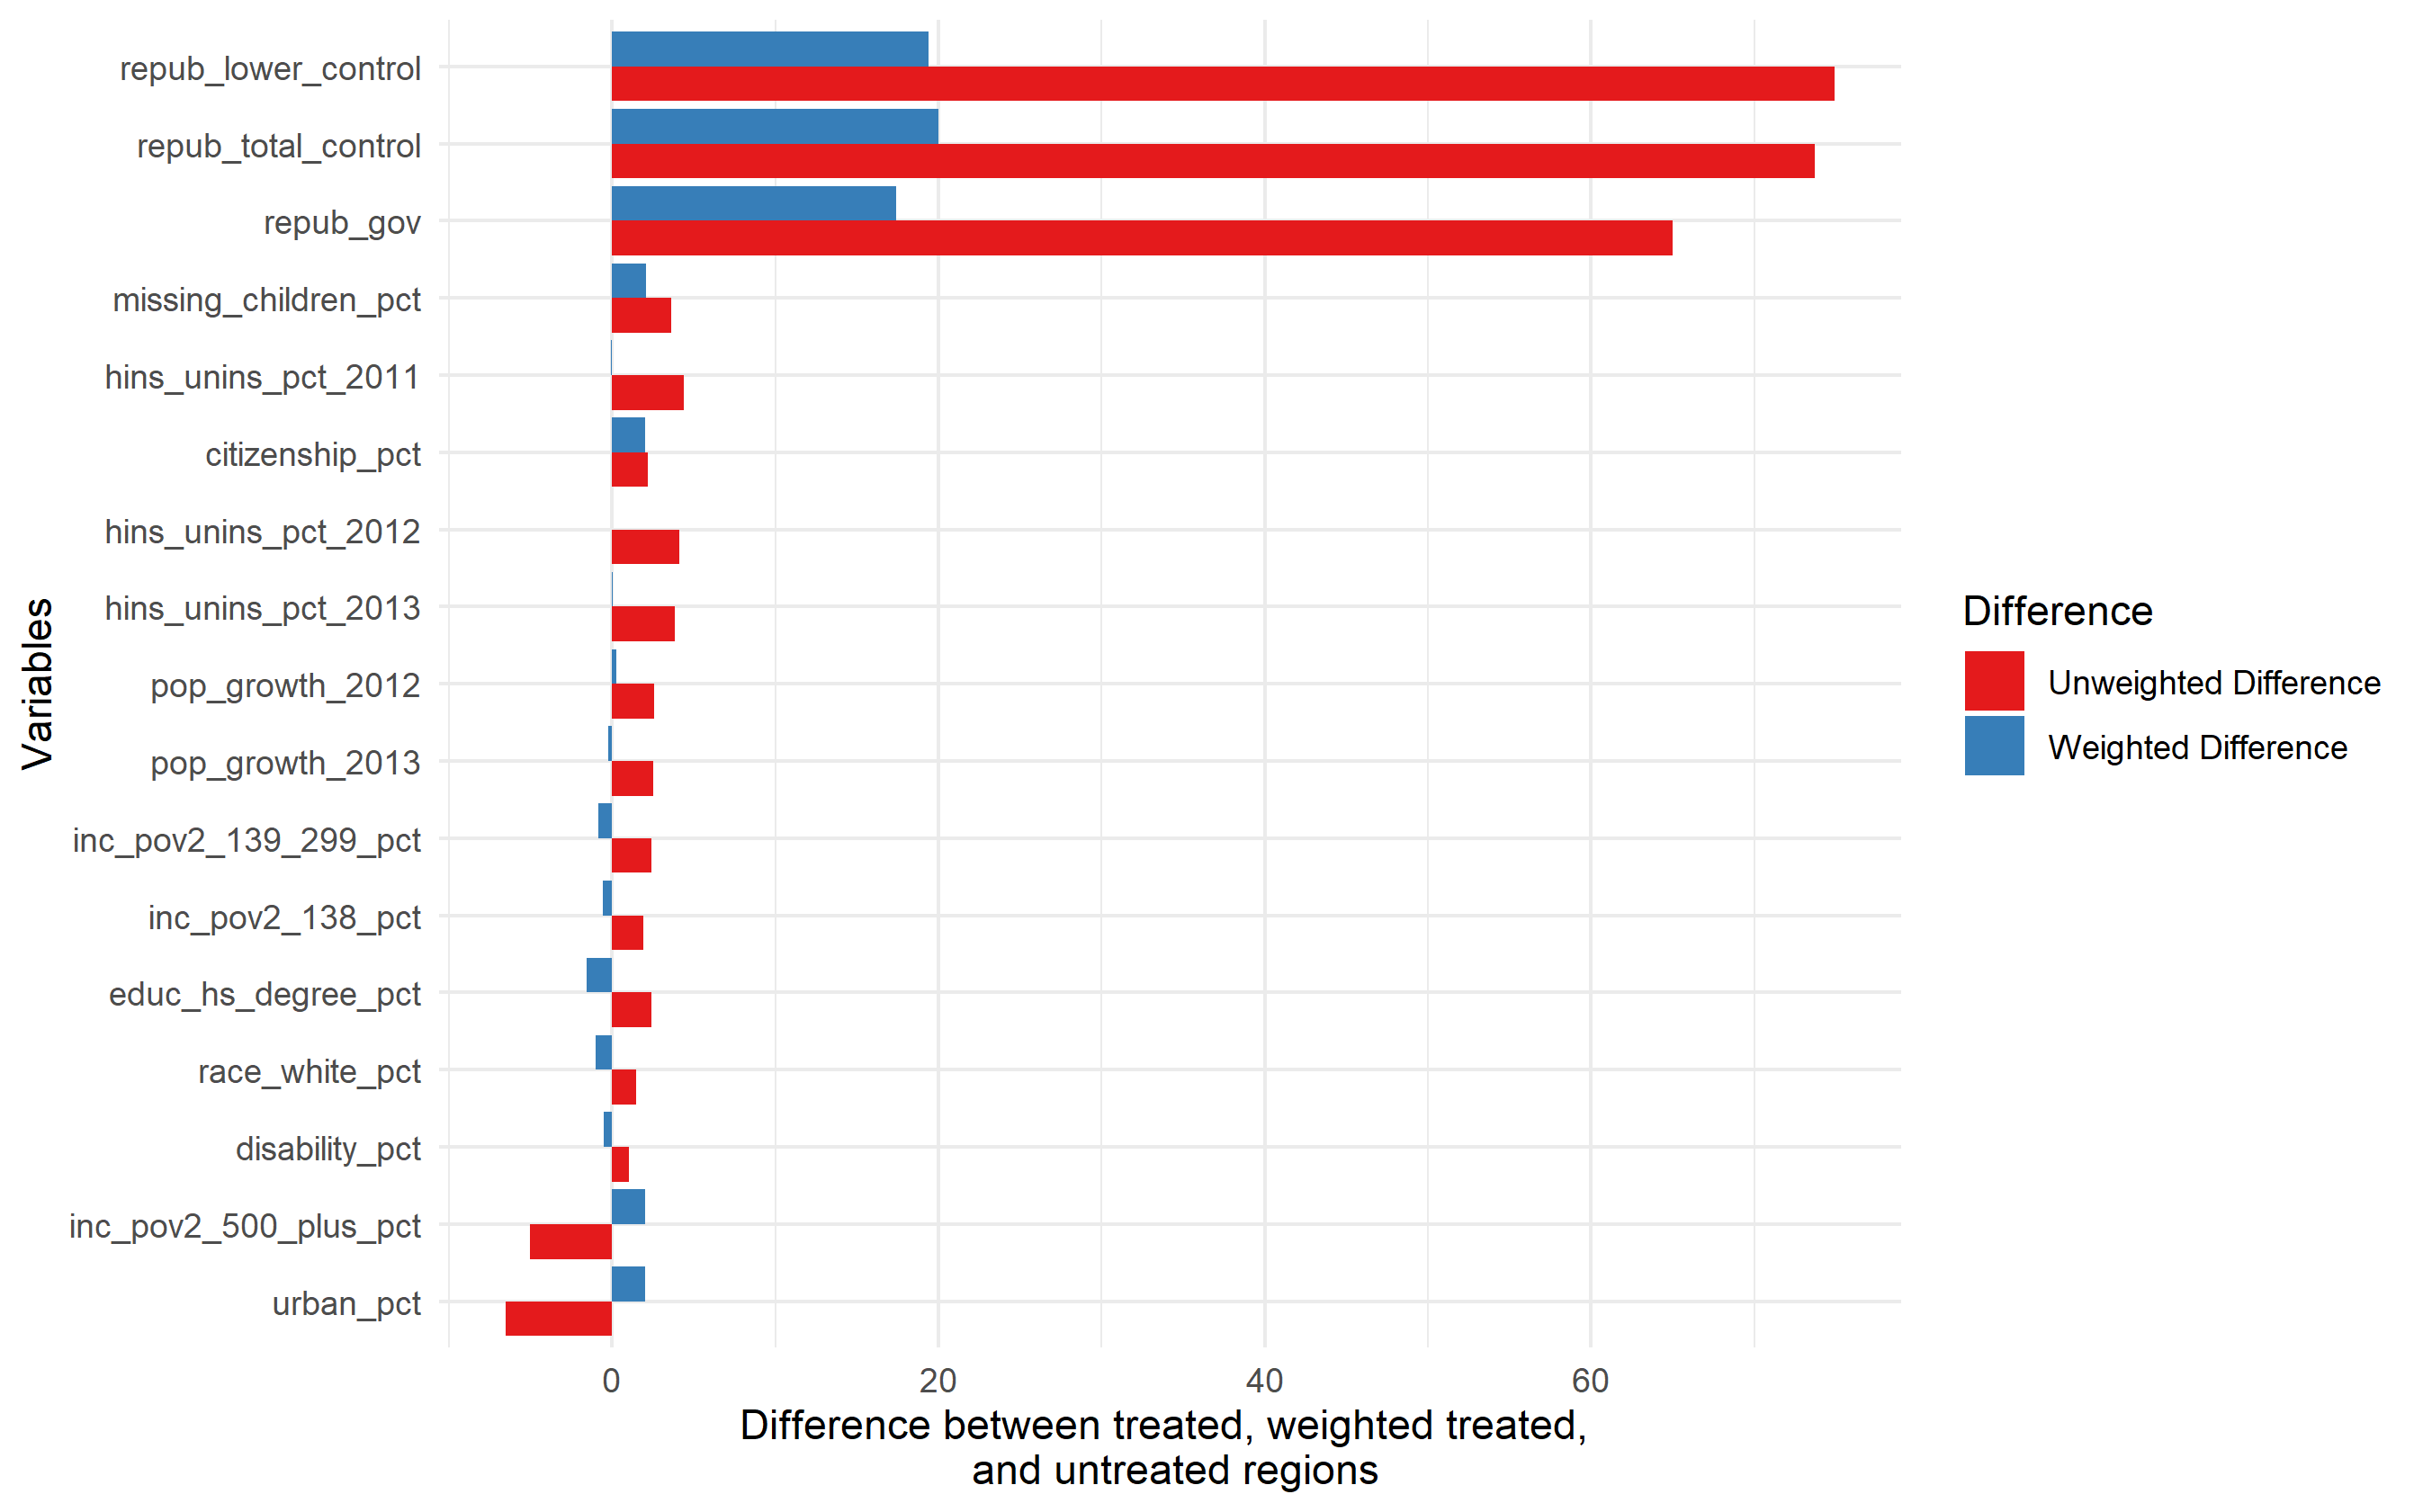
\includegraphics[scale=0.6]{01_Plots/balance-plot-etu.png}
    \caption{Balance plot, primary dataset}
    \label{fig:loveplotc1}
\end{center}
\end{figure}

As discussed above, we use a ridge-regression augmentation to extrapolate from the data in order to reduce all imbalances within 0.1 percentage points. Figure~\ref{fig:statewghts} shows the total weights summed across states for each estimator: H-SBW and BC-HSBW. This figure sums the negative weights separately from the positive weights to show the extent of the extrapolation. We see that BC-HSBW extrapolates heavily in order to estimate the counterfactual, particularly for CPUMAS in California. Due to this extensive extrapolation, we therefore prefer the H-SBW estimator, though we compare results against BC-HSBW as a robustness check.

\begin{figure}[B]
\begin{center}
    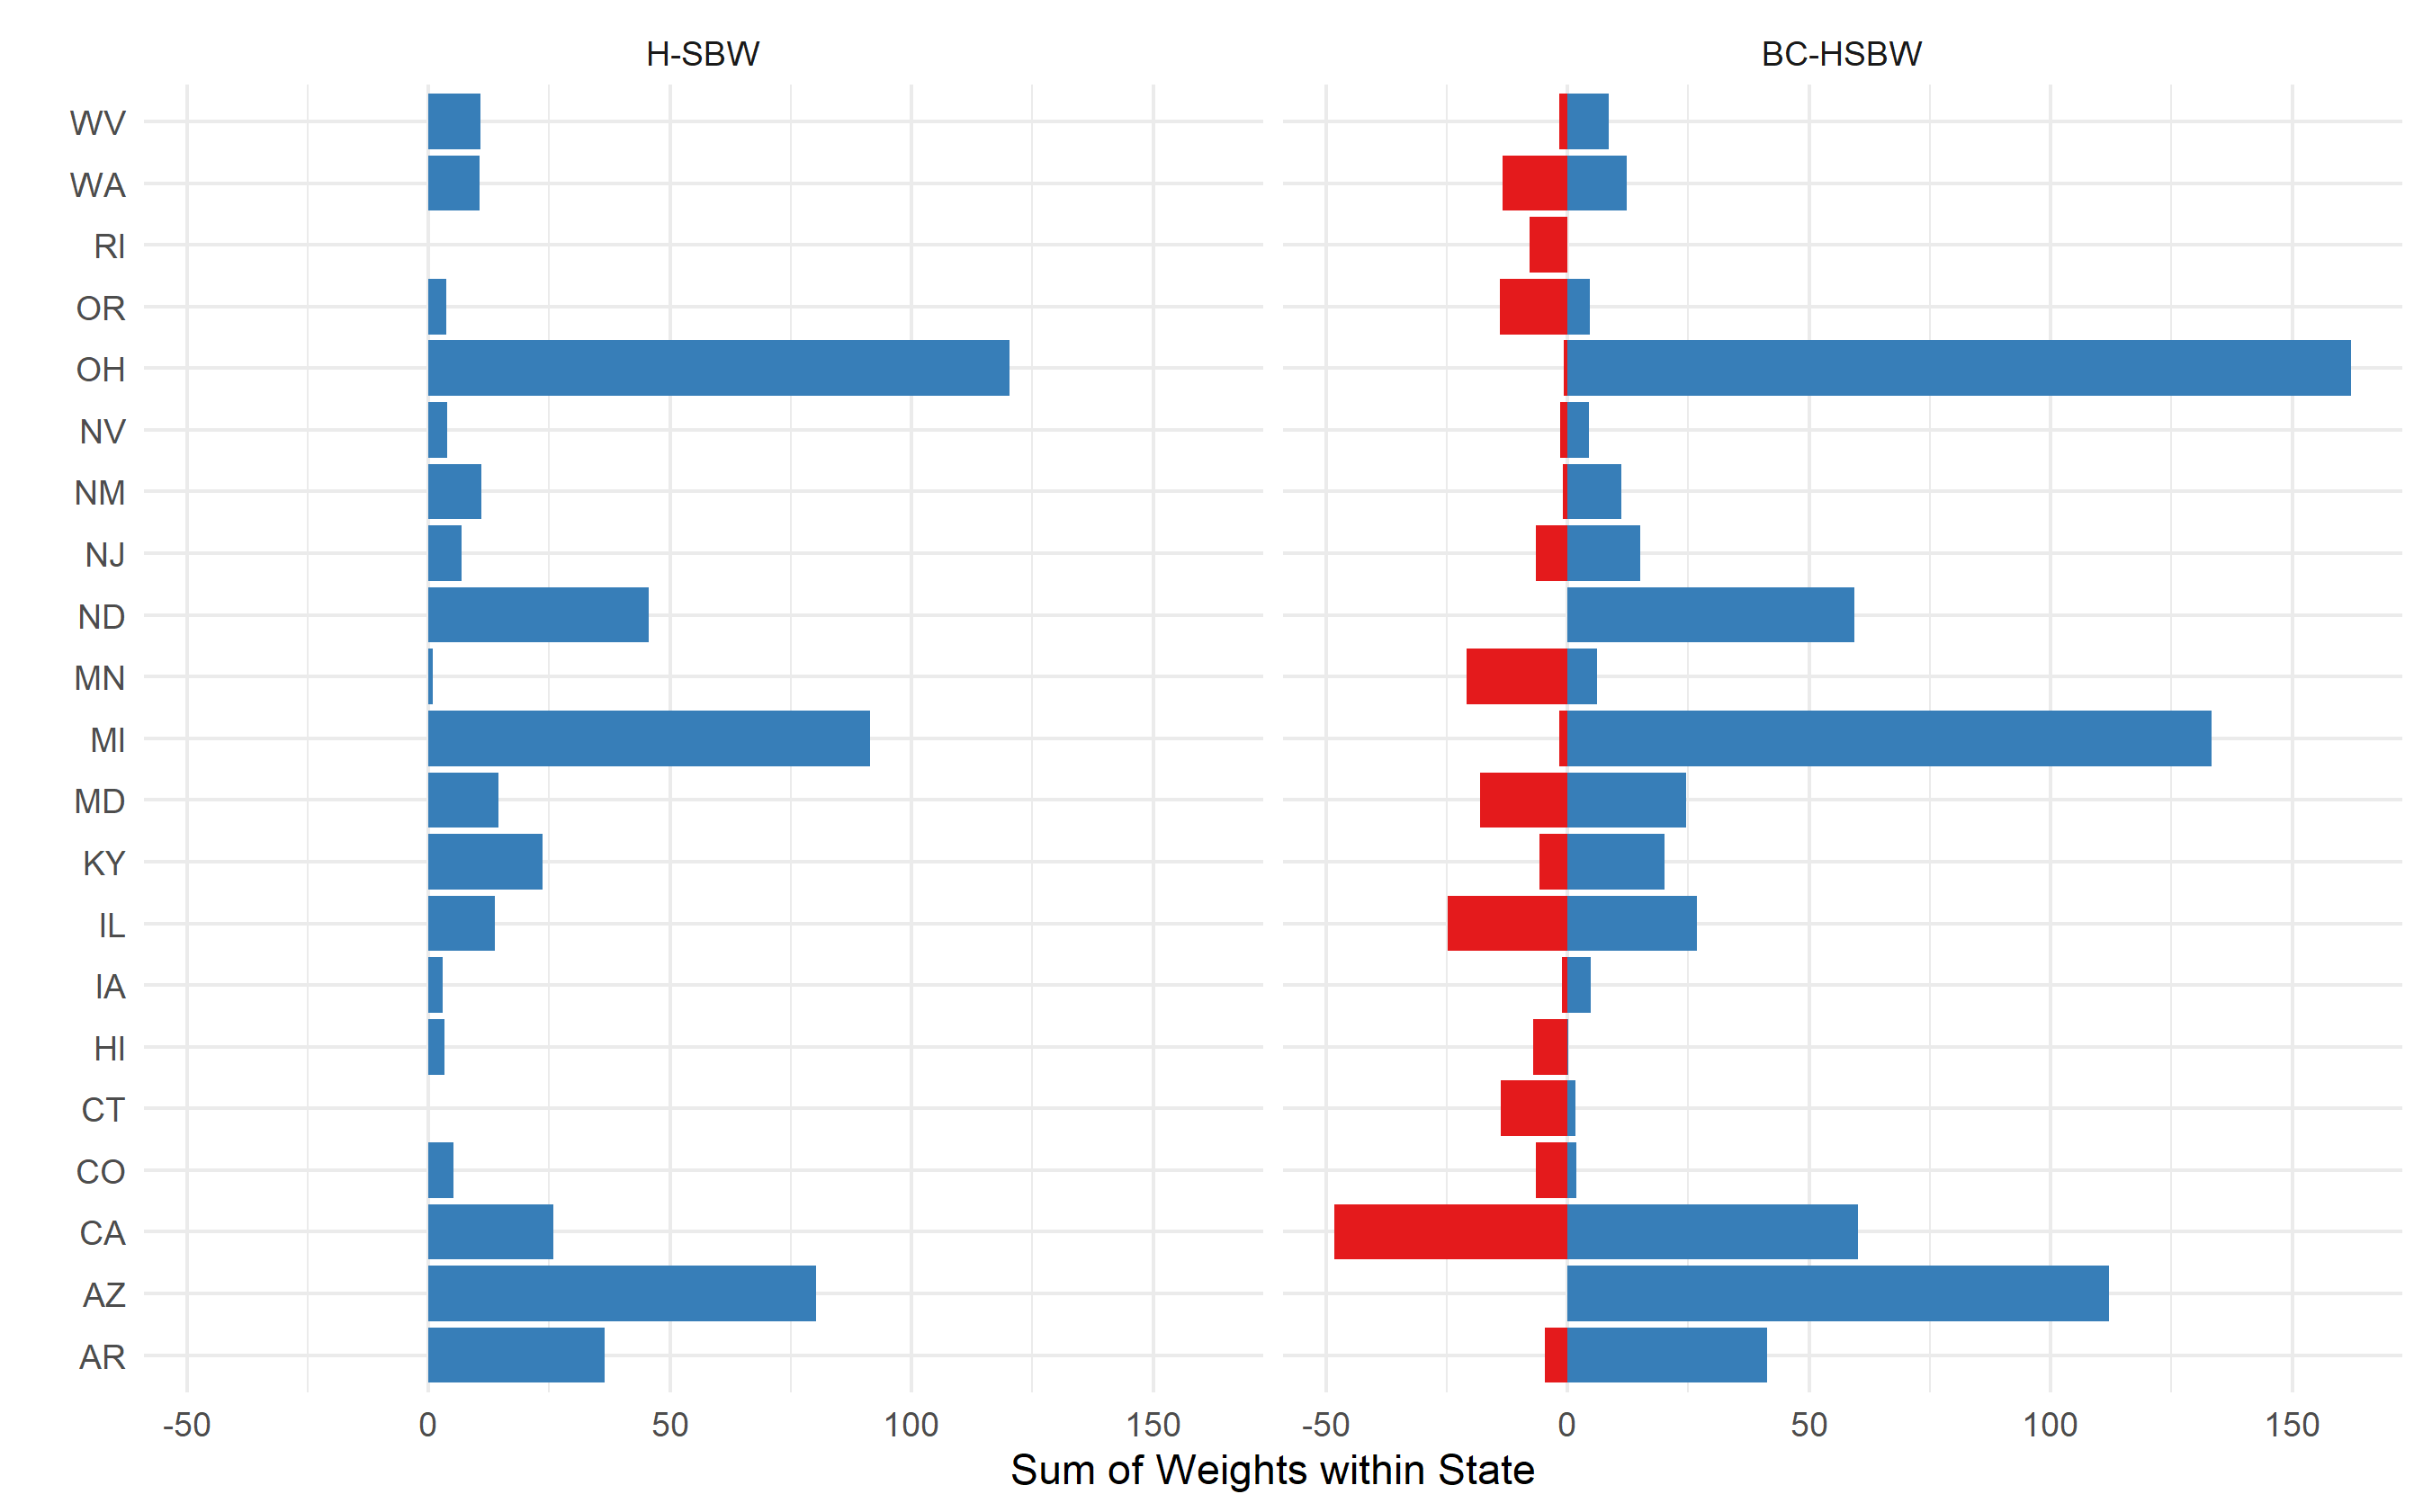
\includegraphics[scale=0.6]{01_Plots/weights-by-state-hsbw-c1.png}
    \caption{Total weights summed by state, primary dataset}
    \label{fig:statewghts}
\end{center}
\end{figure}

Using H-SBW we calculate an estimated effect of -2.00 (-3.59, -0.40). In other words, we estimate that had states that did not expand Medicaid in 2014 done so, they would have seen a 2 percentage point reduction in their uninsurance rates that year. While remaining imbalances are quite large, the bias-correction makes little substantive difference, yielding an estimate of -2.14 (-3.57, -0.71). These estimates differ somewhat from the estimates we find running the procedure on our unadjusted covariate estimates: here H-SBW gives an estimated effect of -2.26 (-3.23, -1.29), and the bias corrected estimator yields -2.50 (-3.41, -1.58). Using the adjusted covariate set appears to both move our estimate closer in absolute magnitude towards zero and decreases the width of the estimated confidence intervals. Figure~\ref{fig:estimators} displays the point estimates from these weighting estimators, as well as estimators using SBW, on the adjusted and unadjusted datasets. Additional results are available in Appendix E.

\begin{figure}[B]
\begin{center}
    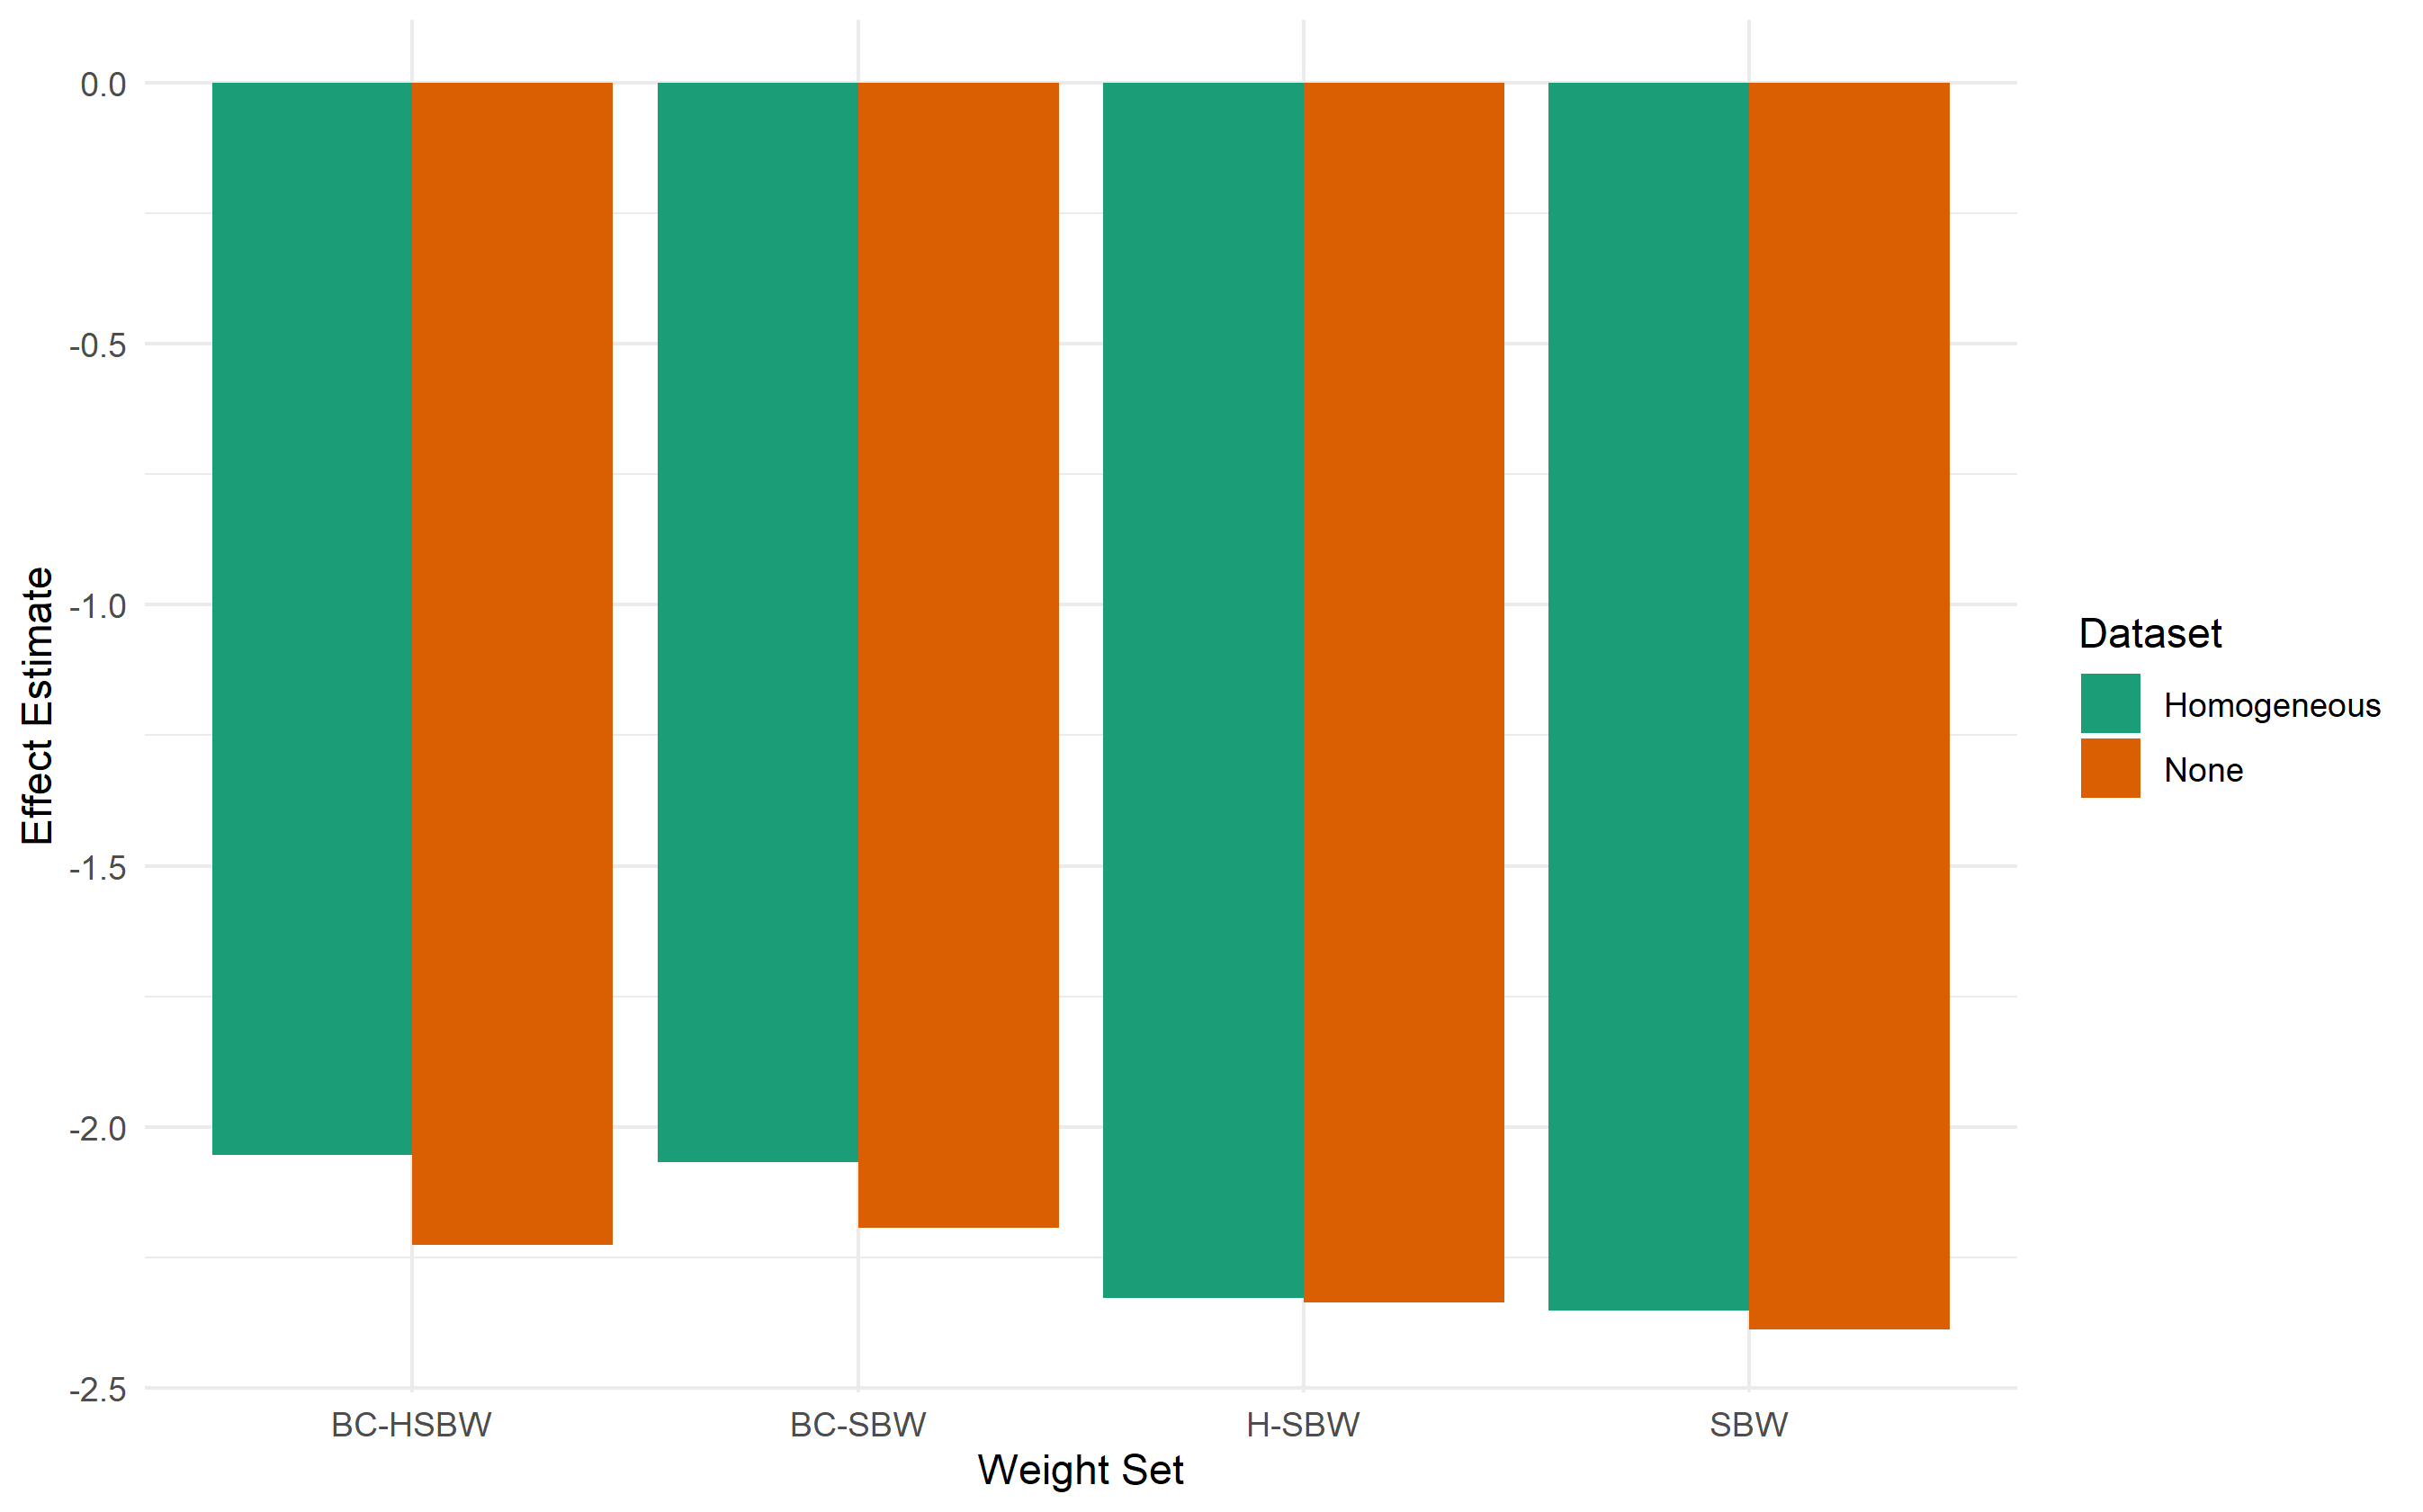
\includegraphics[scale=0.6]{01_Plots/point-estimates-c1.png}
    \caption{Point estimates}
    \label{fig:estimators}
\end{center}
\end{figure}

We examine the robustness of our point estimates to the removal of individual states (note that these are the point estimates used to calculate our confidence intervals). Figure~\ref{fig:loostateplot} shows how the point estimates change for both the adjusted (``sigma\_uu\_i\_modeled'') and unadjusted (``sigma\_zero'') datasets. We see similar results in either case: removing Ohio and Arkansas tends to increase the absolute magnitude of the point estimates. By contrast, removing California decreases the absolute magnitude of the estimators, particularly for estimators that are not bias-corrected. The results are quite similar when using different covariate adjustments and when recalculating the entire procedure; some additional results are available in Appendix E, Table~\ref{tab:loostatec1}. 

\begin{figure}[]
\begin{center}
    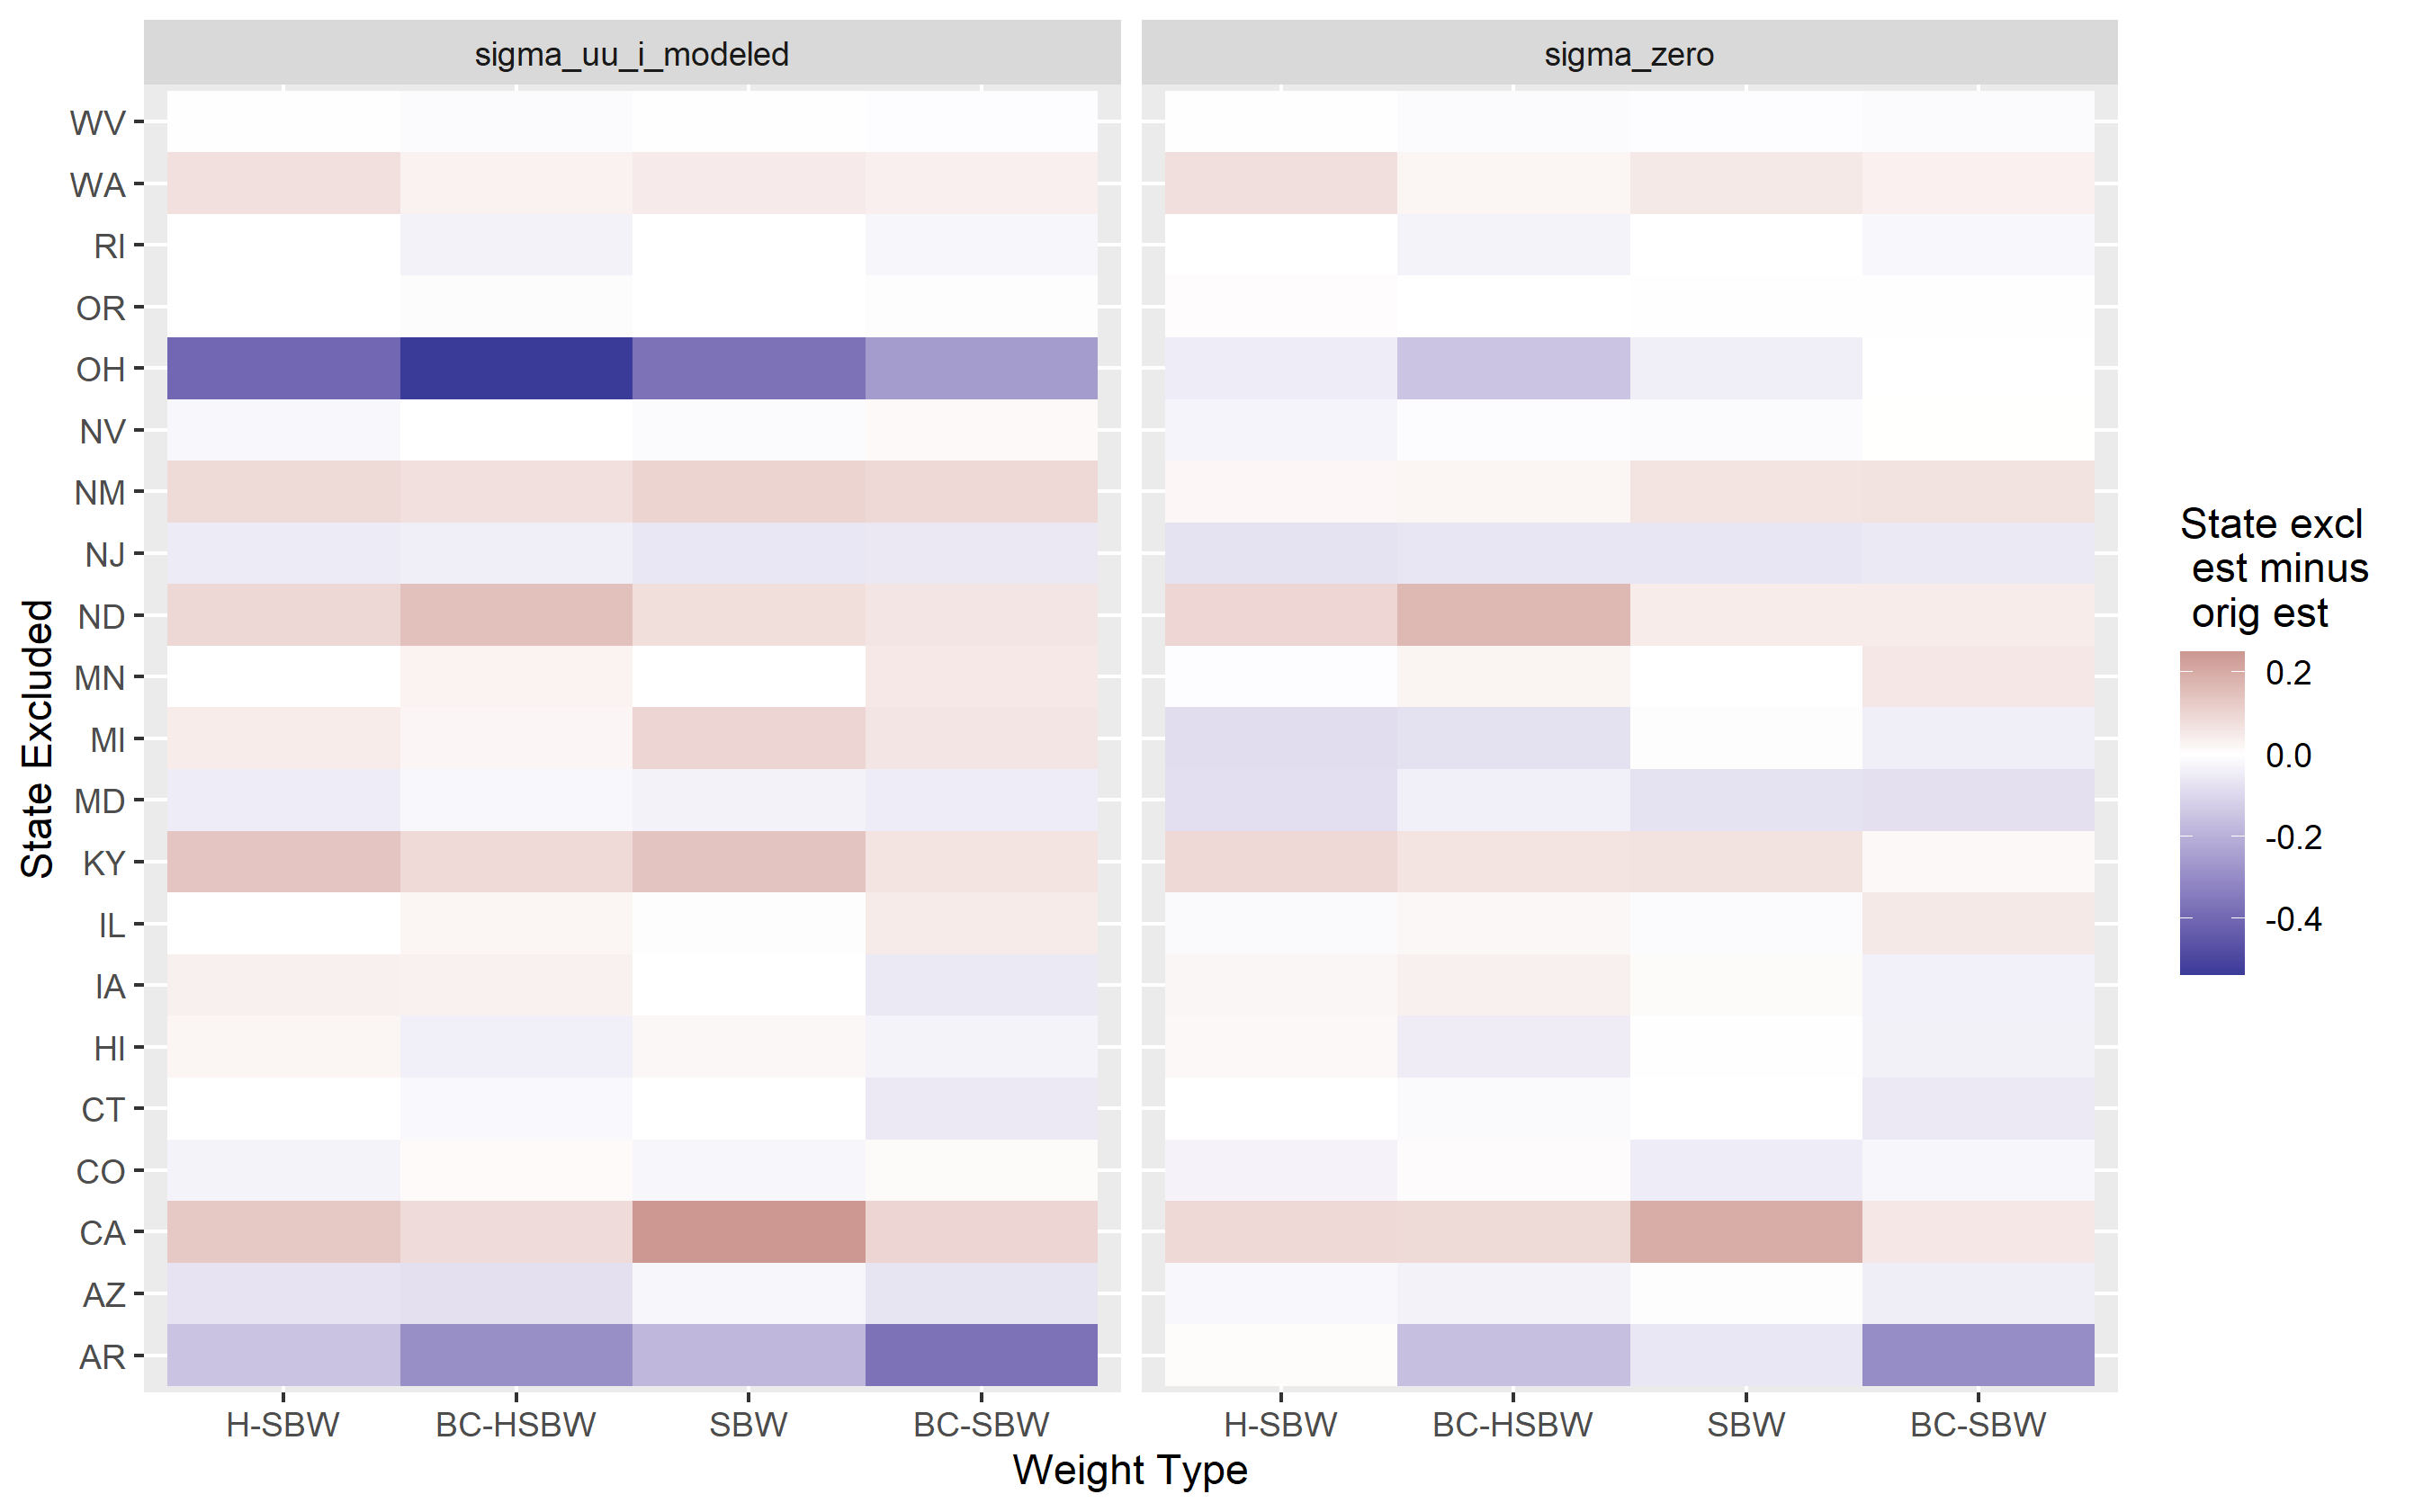
\includegraphics[scale=0.6]{01_Plots/loostate-sensitivityc1-state-uu-i.png}
    \caption{Estimator sensitivity to states}
    \label{fig:loostateplot}
\end{center}
\end{figure}

We now consider our second research question: whether Republican governance might be an effect modifier for the treatment effect. We examine this by removing the Republican governance indicators and recalculating our point estimates and comparing this estimated contrast to our original point estimate (ie the estimated treatment effect when all groups are included). This difference is a function both of the model coefficients and the differences in the weighted imbalances between the covariates of the treated and control groups.

More formally, let $\hat{\psi}_v$ be the estimator with covariates $V$ removed using weights $\gamma_v$; let $\beta_v$ be the model coefficients on those covariates; and let $\hat{\psi}^1_0$ be our primary estimator. This procedure approximately estimates the following quantity:\footnote{Notice that these final two lines are approximations rather than equalities for four reasons: one, error in the outcome model; two, estimation error from $\hat{\eta}(W_{sc})$; three, the difference between $\eta(W_{sc})$ and $X_{sc}$; and finally, because while we hold $\delta$ constant for all covariates not in $V$, the reweighting may affect some of the imbalances within that tolerance for non-binding constraints.}

\begin{align*}
    \hat{\Delta}_v &= \hat{\psi}_v - \hat{\psi}_0 \\
    &= (\hat{\psi}^1_v - \hat{\psi}^0_1)  - (\hat{\psi}^1_0 - \hat{\psi}^1_0) \\
    &= \hat{\psi}^1_v - \hat{\psi}^1_0 \\
    &\approx (X_1^T(\gamma_v - \gamma_0))^T\beta \\
    &\approx (V_1^T(\gamma_v - \gamma_0))^T\beta_v
\end{align*}

Let $\hat{\Delta}$ be this estimate with the Republican governance indicators removed. Because we hypothesize that regions under Republican governed administrations will have lower Medicaid take-up rates, we expect that removing these covariates will move this estimate farther away from zero.\footnote{Specifically, for these covariates we know that $V_1^T(\gamma_1 - \gamma_0)$ will be negative because the treated region is much more Democratic than the control region. Because we expect that Republican governance is positively associated with uninsurance rates, we expect that this overall quantity will be negative.} We also examine the influence of four other covariate groups: pre-treatment uninsurance rates and pre-treatment unemployment rates, and three sets of different demographic indicators. Specifically, the first group includes: urban residence, age group, education, citizenship, student, disability, female; the second, white race, Hispanic ethnicity, foreign-born, and income-to-poverty ratio; the third, children category (0, 1, 2, 3+, NA), household to population ratio, and population growth. We present and comment on these results in Appendix E, Table~\ref{tab:ptests}.

For the H-SBW estimator we calculate $\hat{\Delta}$ equal to -0.62 (-2.05, 0.81) for BC-HSBW and -0.51 (-1.74, 0.71). We see similar differentials on our unadjusted dataset (0.64 (-1.62, 0.34) and 0.49 (-1.33, 0.34), respectively). These results are consistent with our hypothesis that Republican governance drives heterogeneity in the effect of Medicaid expansion. While our confidence intervals include zero, we find that these differences are negative for all estimators we consider when removing each state (conditional on the covariate adjustment). That is, the sign of the differences in the contrasts remains negative for every specification that we run.\footnote{When we re-run the entire adjustment procedure when removing each state, we find that removing California results in a positive contrast between these estimates for BC-HSBW and BC-SBW and Illinois for BC-SBW for our adjusted dataset. However, this result only occurs with weights that extrapolate beyond the support of the data calculated on a covariate-adjusted dataset. We find that the covariate adjustments can lead to quite extreme imputed values for certain CPUMAs, particularly when we reduce the amount of data used to calculate the adjustment, a limitation of using a linear approximation to impute covariates that can only fall within a certain range. This problem compounds when allowing the weights to extrapolate because they are far more likely to use these bad estimates. Additional comments on these extreme values are available in Appendix C.} Overall we view this as suggestive (though not definitive) evidence consistent with our research hypothesis.

Appendix E Figure~\ref{fig:rdiffc1state} and Figure~\ref{fig:rdiffc1proc} display all estimates $\hat{\Delta}$ with each state removed, both conditional on the covariate adjustment and recalculating the covariate adjustment, respectively. Additional results for different estimators are available in Appendix E, Table~\ref{tab:deltac1}.

\subsection{Sensitivity Analyses} \label{sssec:sensitivity}

We examine the sensitivity of our analysis to violations of two key causal assumptions: (1) no anticipatory treatment effects, and (2) positivity violations. To the first point, several states had partial limited expansions prior to 2014. Following \cite{frean2017premium}, these states are California, Connecticut, Minnesota, New Jersey, and Washington. We rerun our analyses excluding CPUMAs from all five of these states. It is unclear how removing these states might affect our estimates: on the one hand, states that expanded early might have a smaller treatment effect after 2014 because they already enrolled newly eligible individuals. On the other hand, if these states were also more motivated to enroll people in Medicaid, they might have larger post-expansion coverage gains. Figure~\ref{fig:weightsbystatec2} displays the H-SBW weights summed by state alongside BC-HSBW. We again see that the BC-HSBW estimator extrapolates heavily to reduce the imbalances. A complete balance table is available in Appendix D, Table~\ref{tab:baltab1} and Table~\ref{tab:baltab2}.

\begin{figure}[]
\begin{center}
    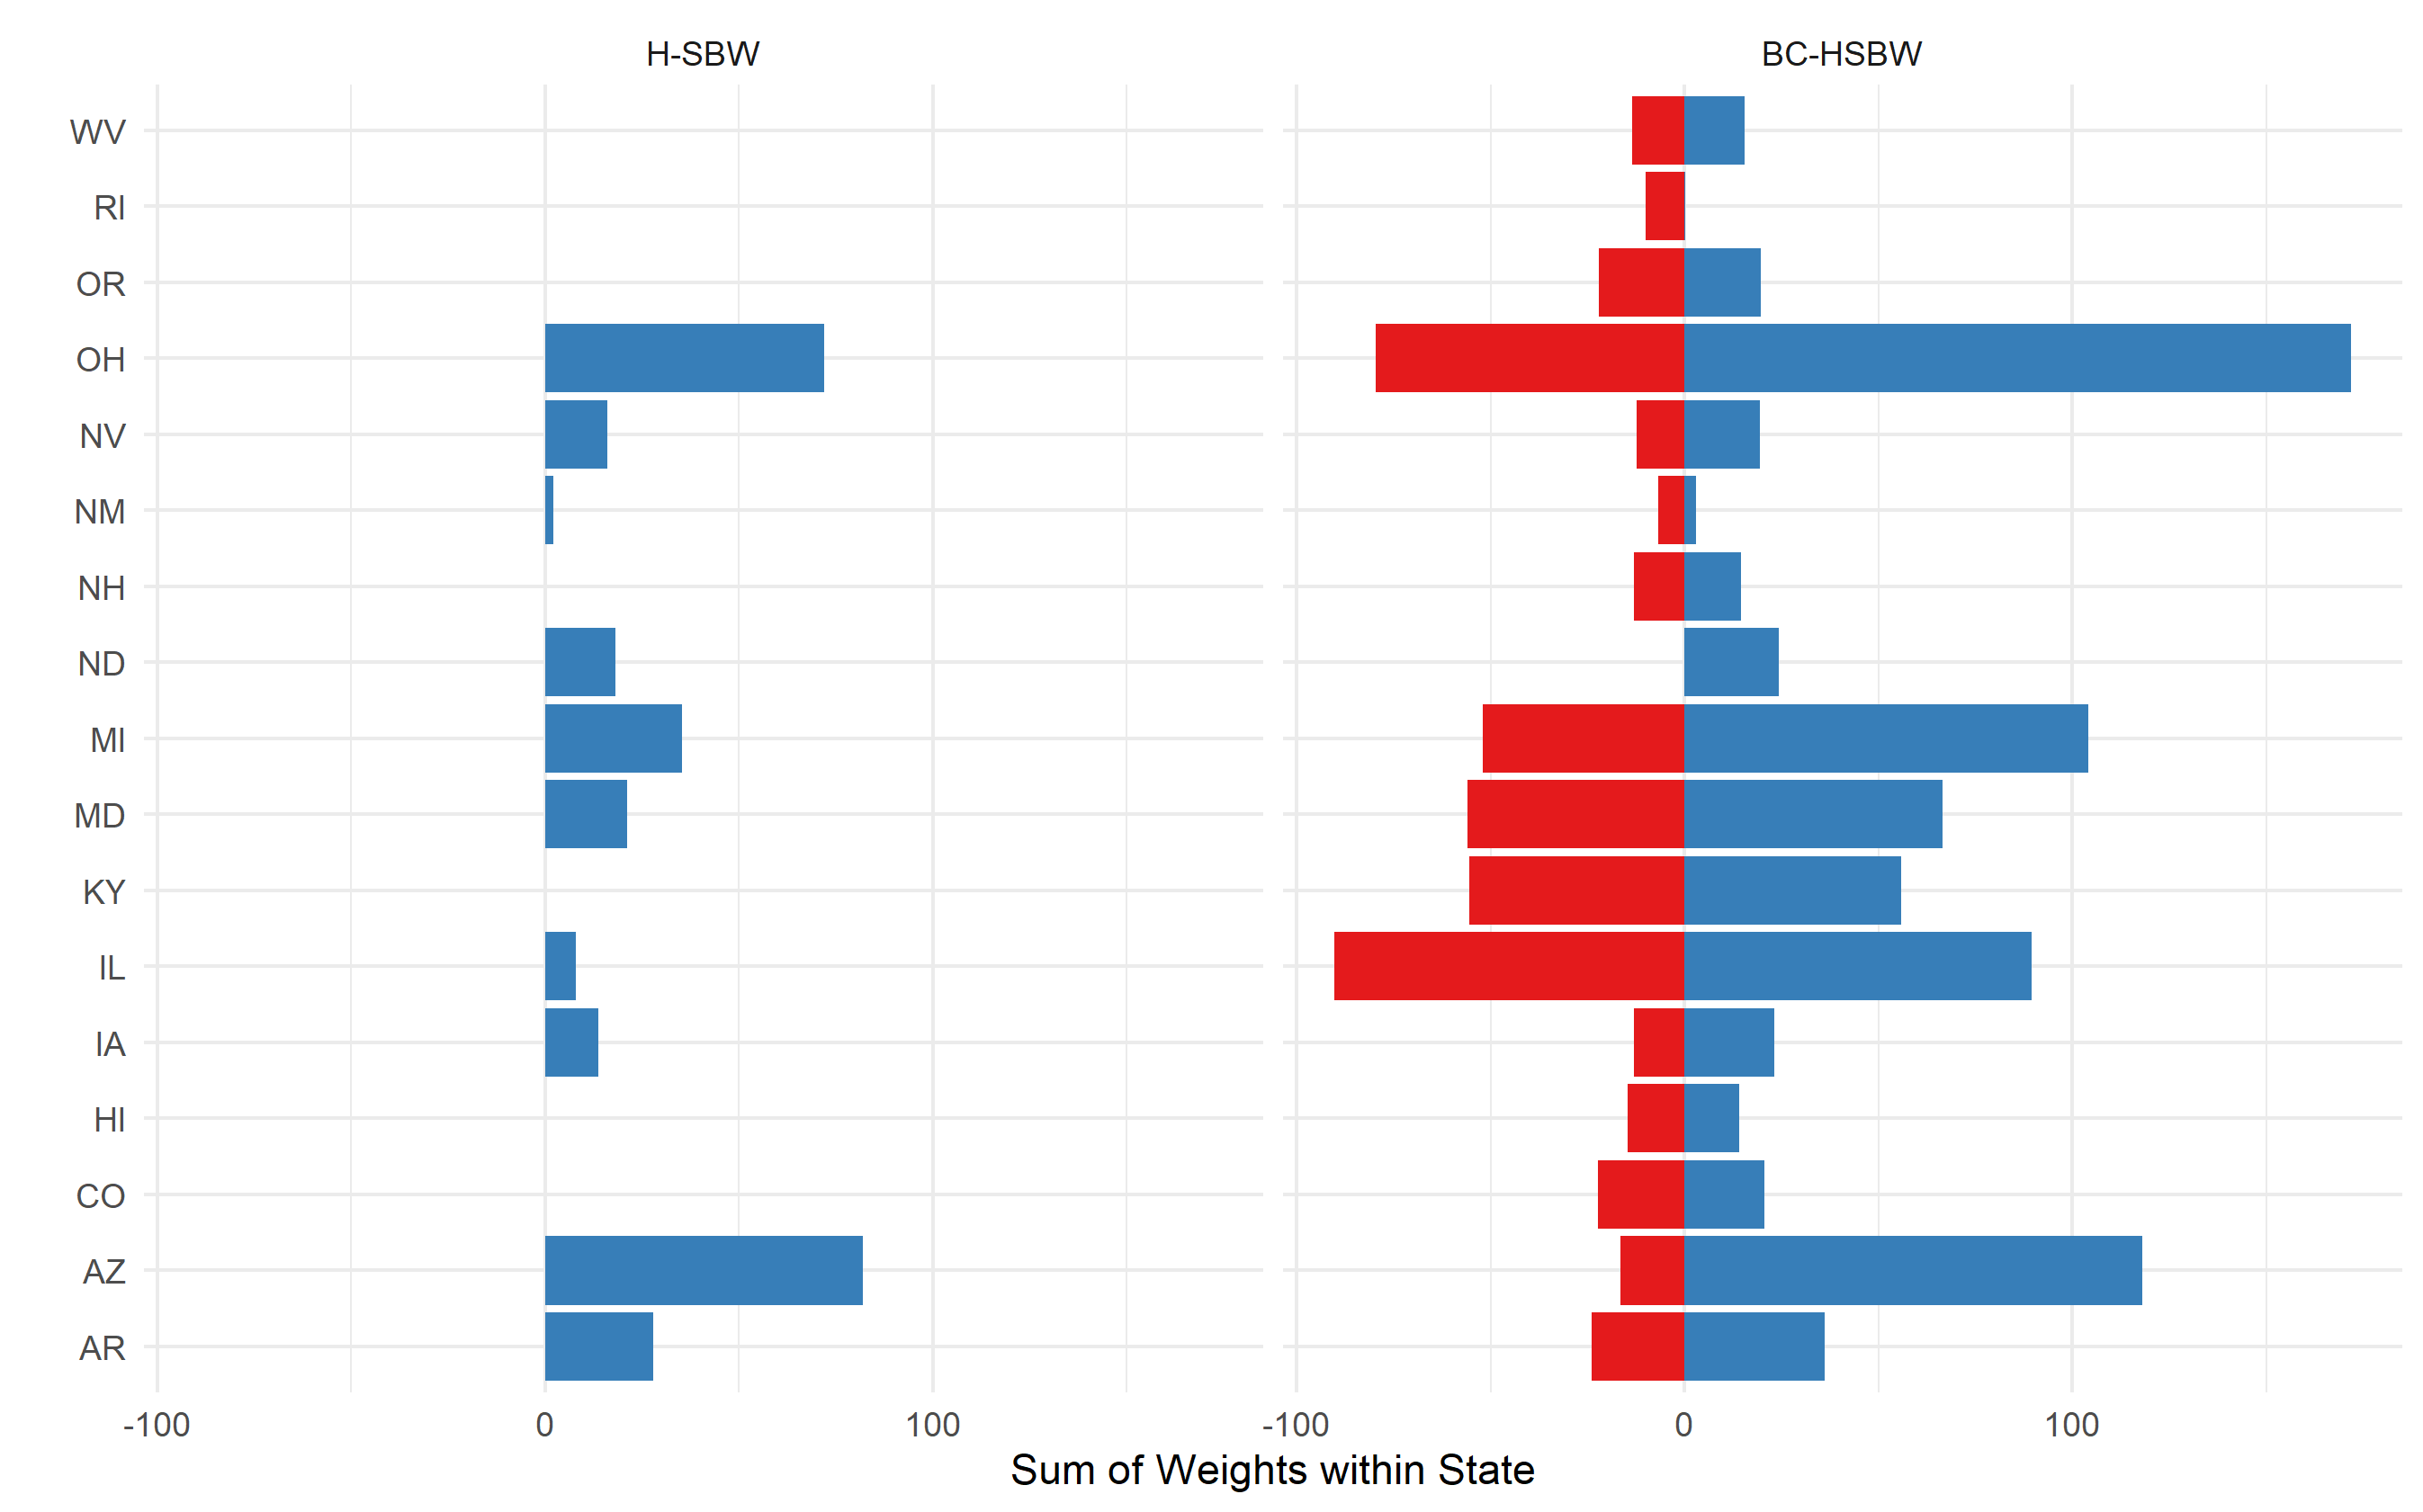
\includegraphics[scale=0.6]{01_Plots/weights-by-state-hsbw-c2.png}
    \caption{Total weights summed by state, early expansion removed}
    \label{fig:weightsbystatec2}
\end{center}
\end{figure}

On this dataset we estimate an effect of -1.48 (-2.91, -0.06) using H-SBW weights; BC-HSBW yields an estimate of -2.06 (-3.72, -0.41). Here we see that the bias correction makes a larger substantive difference to the point estimate; however, it is not substantively different from the original point estimate with all states included. Overall we view this as evidence that our primary point estimates are fairly robust to the exclusion of these states, though perhaps the true effect is smaller in absolute magnitude. Table~\ref{tab:confintmainc2} and Table~\ref{tab:secondaryptests} in Appendix E display additional results. 

We also find that our estimates $\hat{\Delta}$ increase in absolute magnitude. Specifically, we find -1.15 (-2.53, 0.24) percentage point decrease for the H-SBW estimator when excluding the Republican governance indicators and a -0.74 (-2.40, 0.91) increase for BC-HSBW. Figure~\ref{fig:repub} displays these differences in the contrasts against those from our primary dataset. On our unadjusted dataset we estimate contrasts of -1.04 (-2.01, -0.07) and -0.61 (-1.75, 0.52). While these confidence intervals mostly contain zero, we again find that each individual difference between the leave-one-out-states estimated contrasts is less than zero (conditional on the covariate adjustment). These results again are consistent with hypothesis that factors associated with Republican governance reduce the effect size of Medicaid expansion. Additional results are available in Appendix E, Table~\ref{tab:deltac2}. 

\begin{figure}[]
\begin{center}
    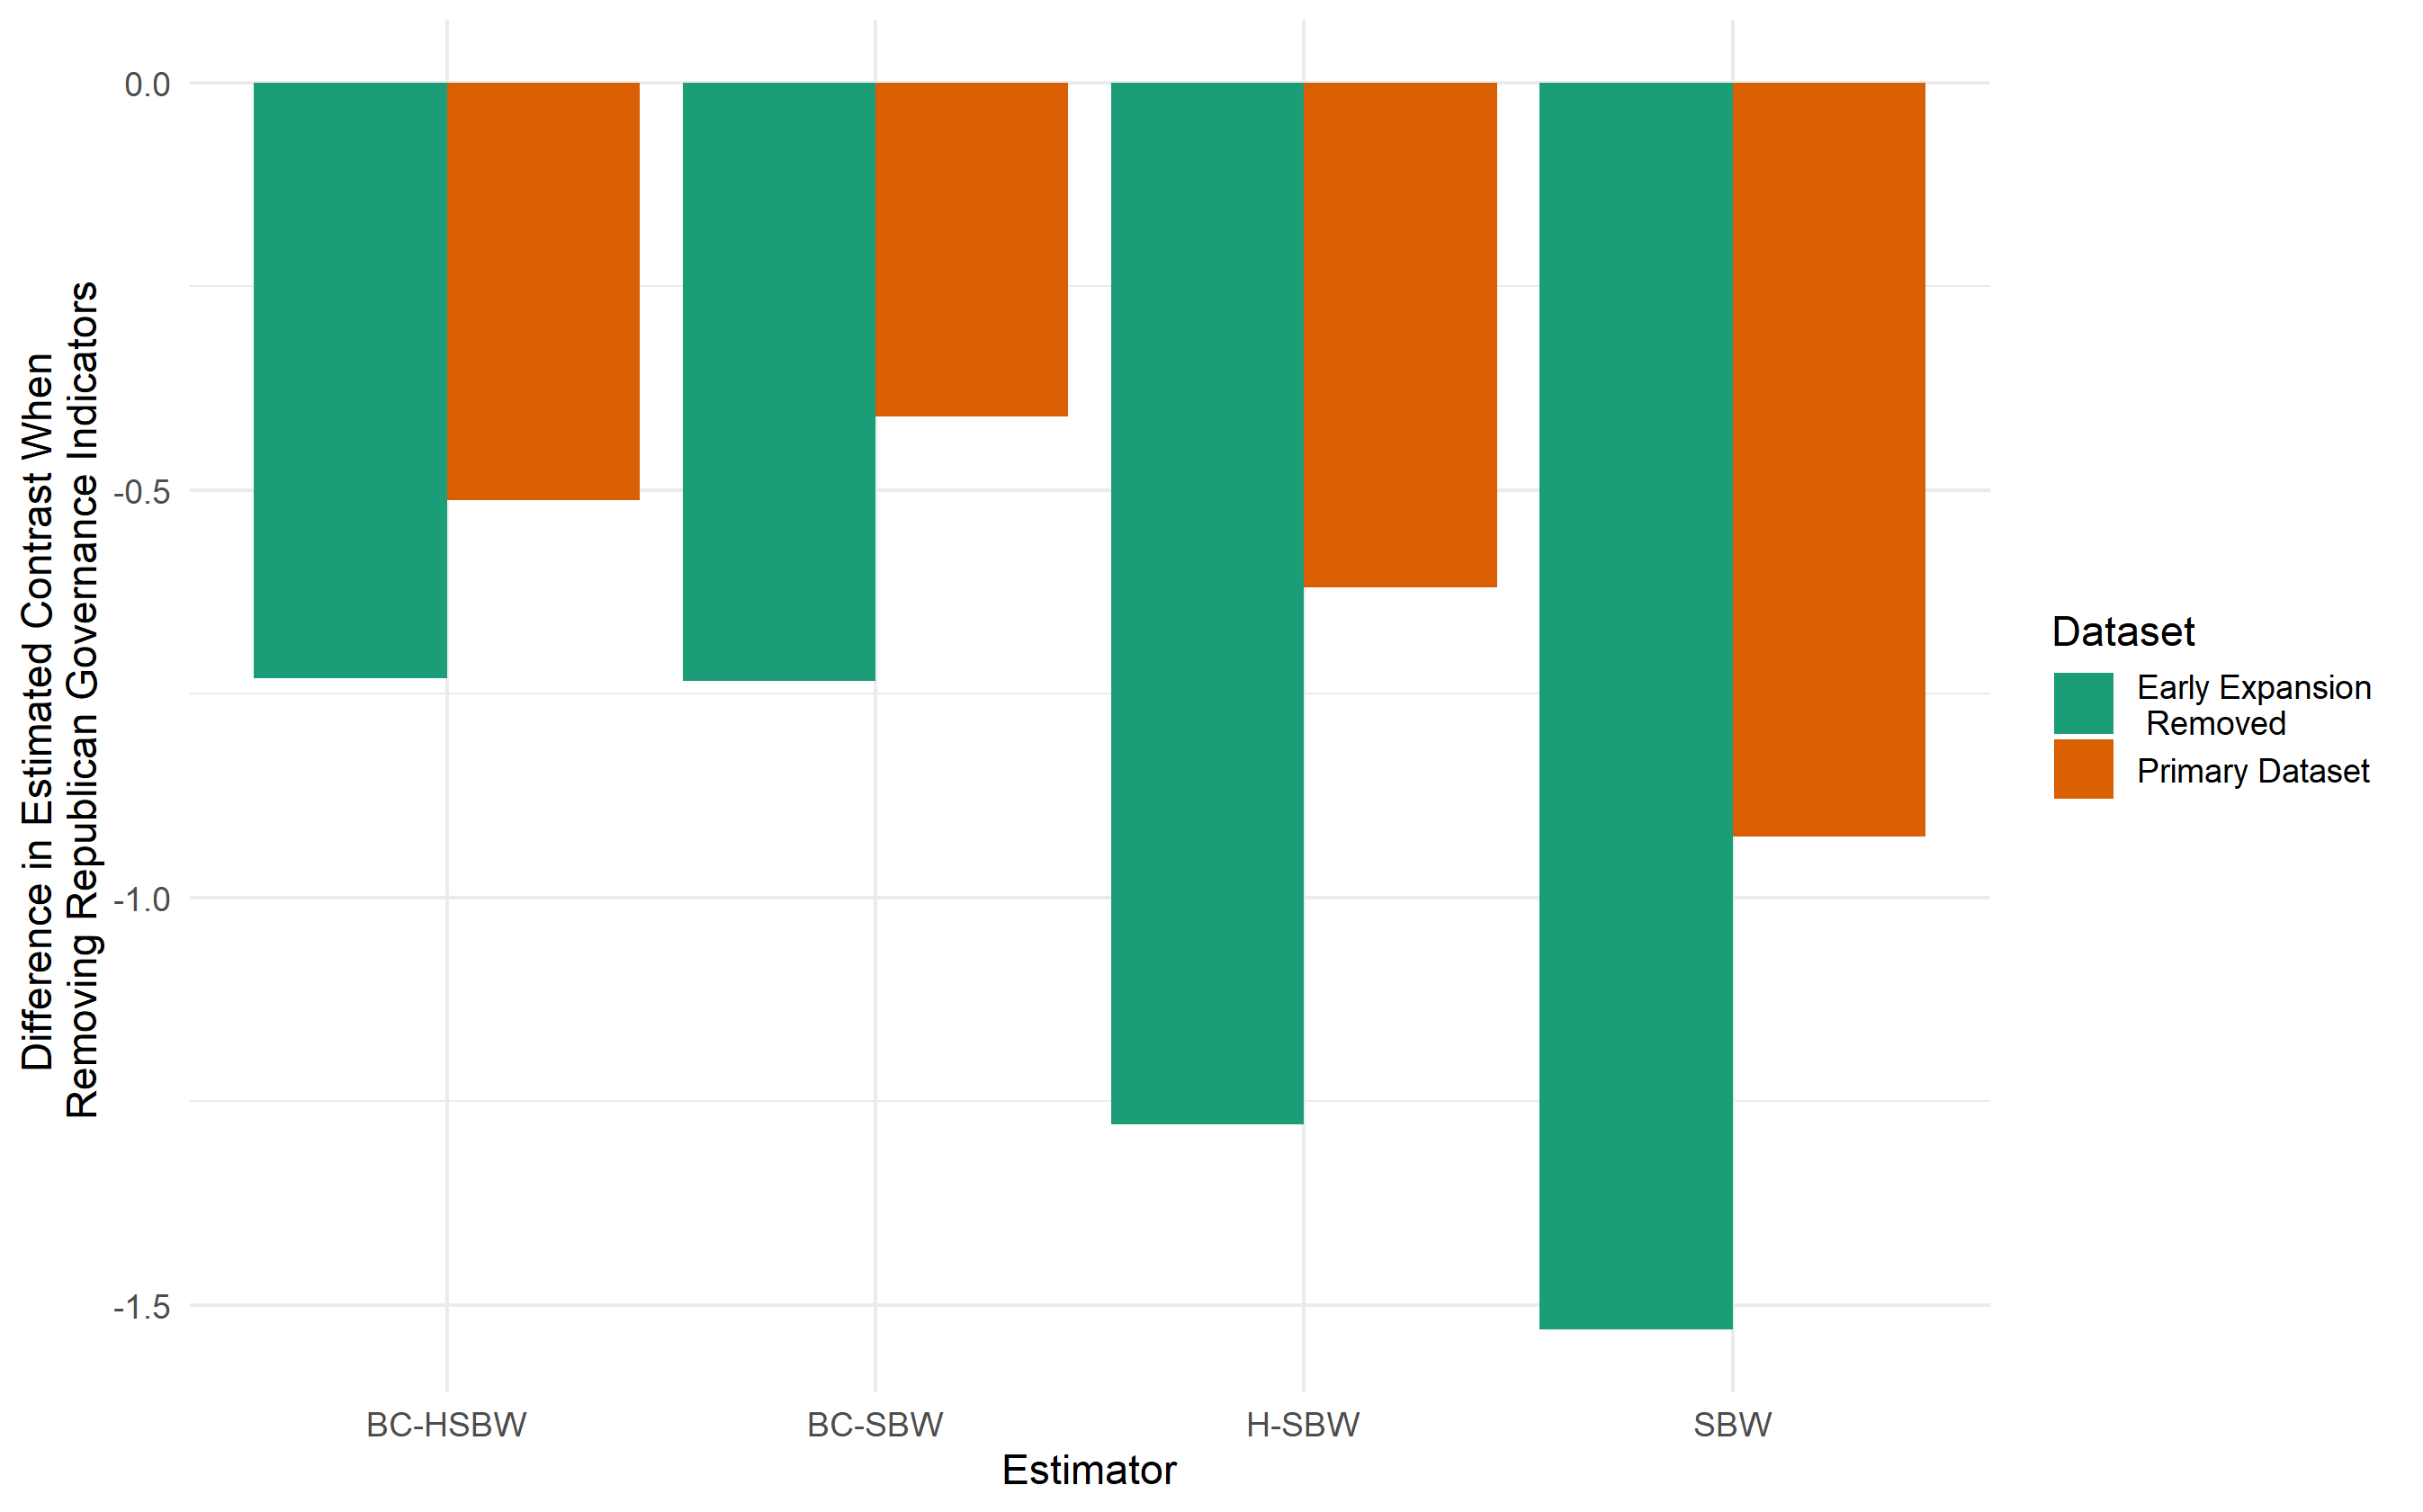
\includegraphics[scale=0.6]{01_Plots/repub-diff-c1c2.png}
    \caption{Removing Republican Governance Indicators}
    \label{fig:repub}
\end{center}
\end{figure}

We conclude by considering an alternative method to account for positivity violations. To this point we have relied on either (1) retaining a potentially biased estimate from weights that do not provide exact balance, or (2) producing a more model-dependent estimate that relies on extrapolation. Overall we found that the results didn't change substantially either way. Here we consider a third option: changing our target estimand. In particular, we consider the overlap average treatment effect (OATE), proposed by \cite{li2018balancing}. This is the treatment effect on the subset of the entire dataset where we have overlap. It is a data-dependent treatment effect, and is not the same as the treatment effect on the untreated; however, we believe that this effect will be more similar to the ETC than the ETT, particularly because there were no Democratic controlled states that did not expand Medicaid. Indeed, after generating overlap weights on our primary dataset we find that across all covariates, the mean average absolute distance from the overlap region to the untreated region is 2.9 and to the treated region is 7.8.\footnote{The distance is between the overlap region calculated as an unweighted mean on the adjusted datasets.} Figure~\ref{fig:oatearea} displays the distance between covariates with greater than one percentage point distance from the overlap region to either the control or treated region. We see that the overlap region is substantially more Republican than the treated region, as expected. This region is also less Hispanic, more white, less rural, and more educated than either the expansion or non-expansion region. Table~\ref{tab:oatedist1} and Table~\ref{tab:oatedist2} in Appendix D show additional statistics on the OATE region versus the treatment and control regions for all covariates.

\begin{figure}[]
\begin{center}
    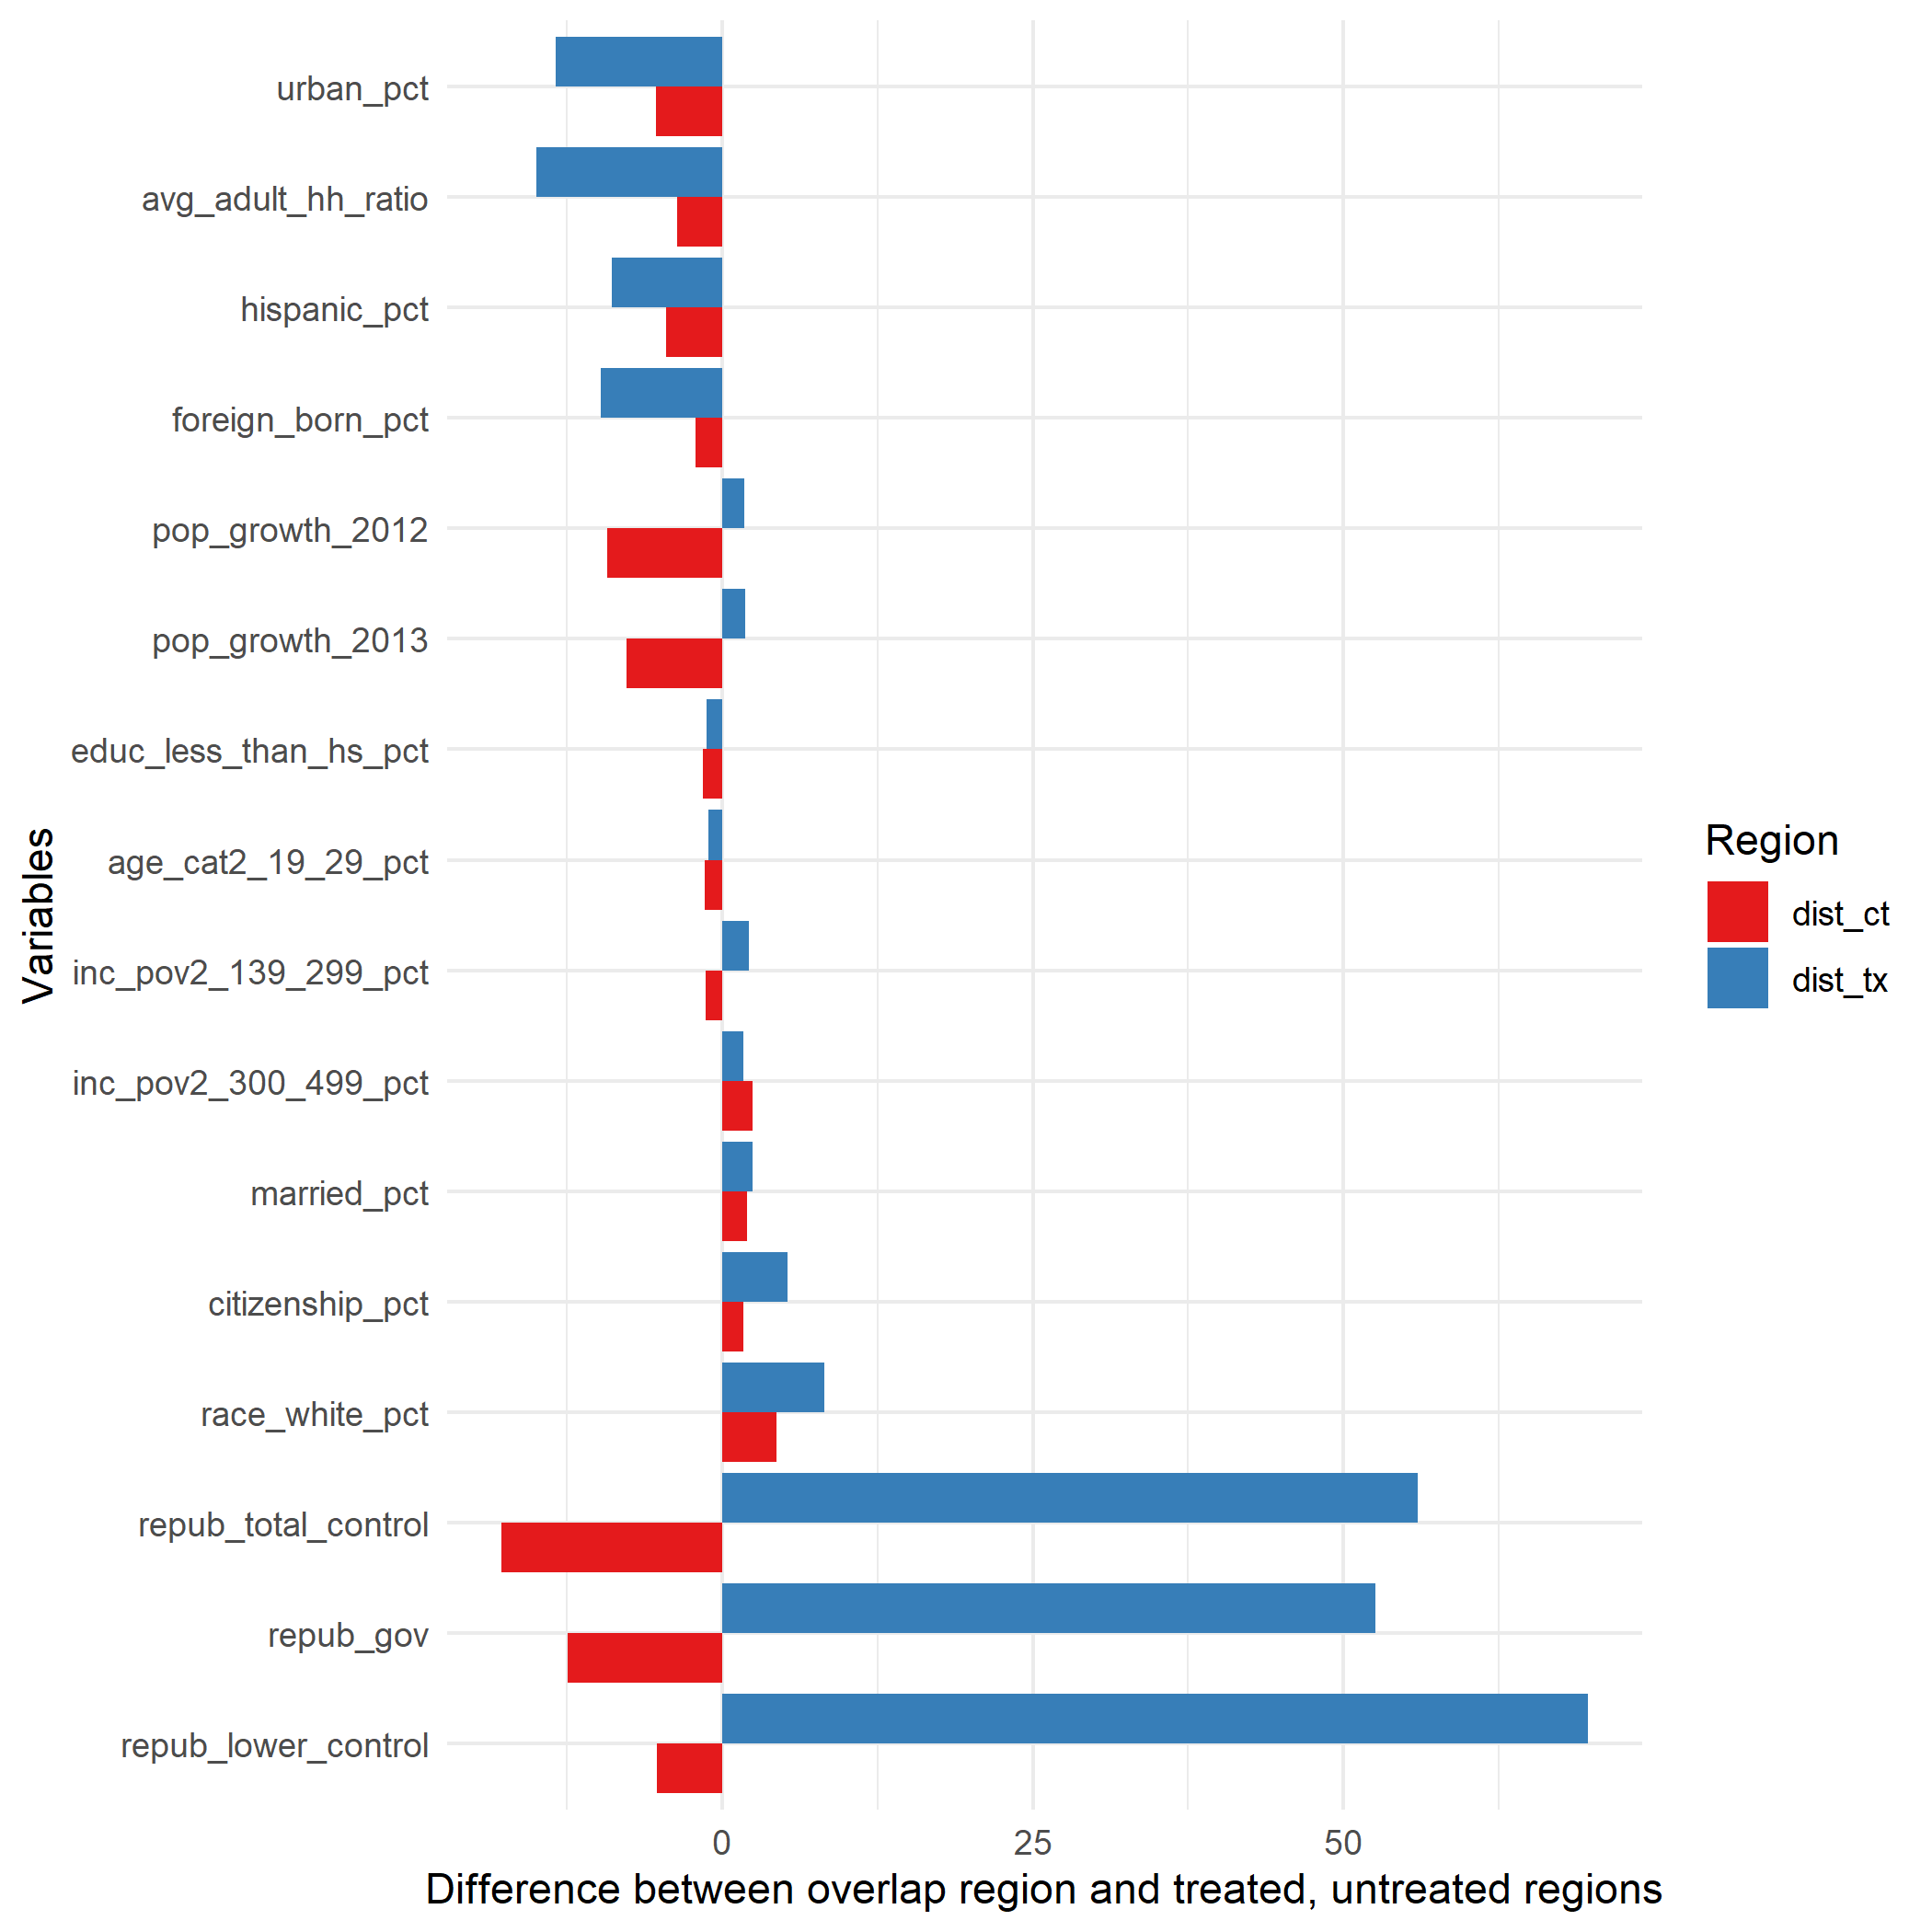
\includegraphics[scale=0.6]{01_Plots/oate-imbalances.png}
    \caption{Overlap area compared to treated, untreated regions}
    \label{fig:oateimbalance}
\end{center}
\end{figure}

Figure~\ref{fig:oateimbalance} displays the sum of the weights within each state by treatment group. Ohio, Michigan, and Arkansas, which all expanded Medicaid, are the most heavily weighted states (the weights are standardized to sum to 100). The weights are more evenly dispersed among the non-expansion regions, though Pennsylvania, Missouri, Wisconsin, and Florida are given the most weight. We note that this region is specific to the preferred covariate adjustment; the results are quite similar for the unadjusted and less preferred covariate adjustment and are available in Appendix D, Table ~\ref{tab:oatestateweights}.

\begin{figure}[]
\begin{center}
    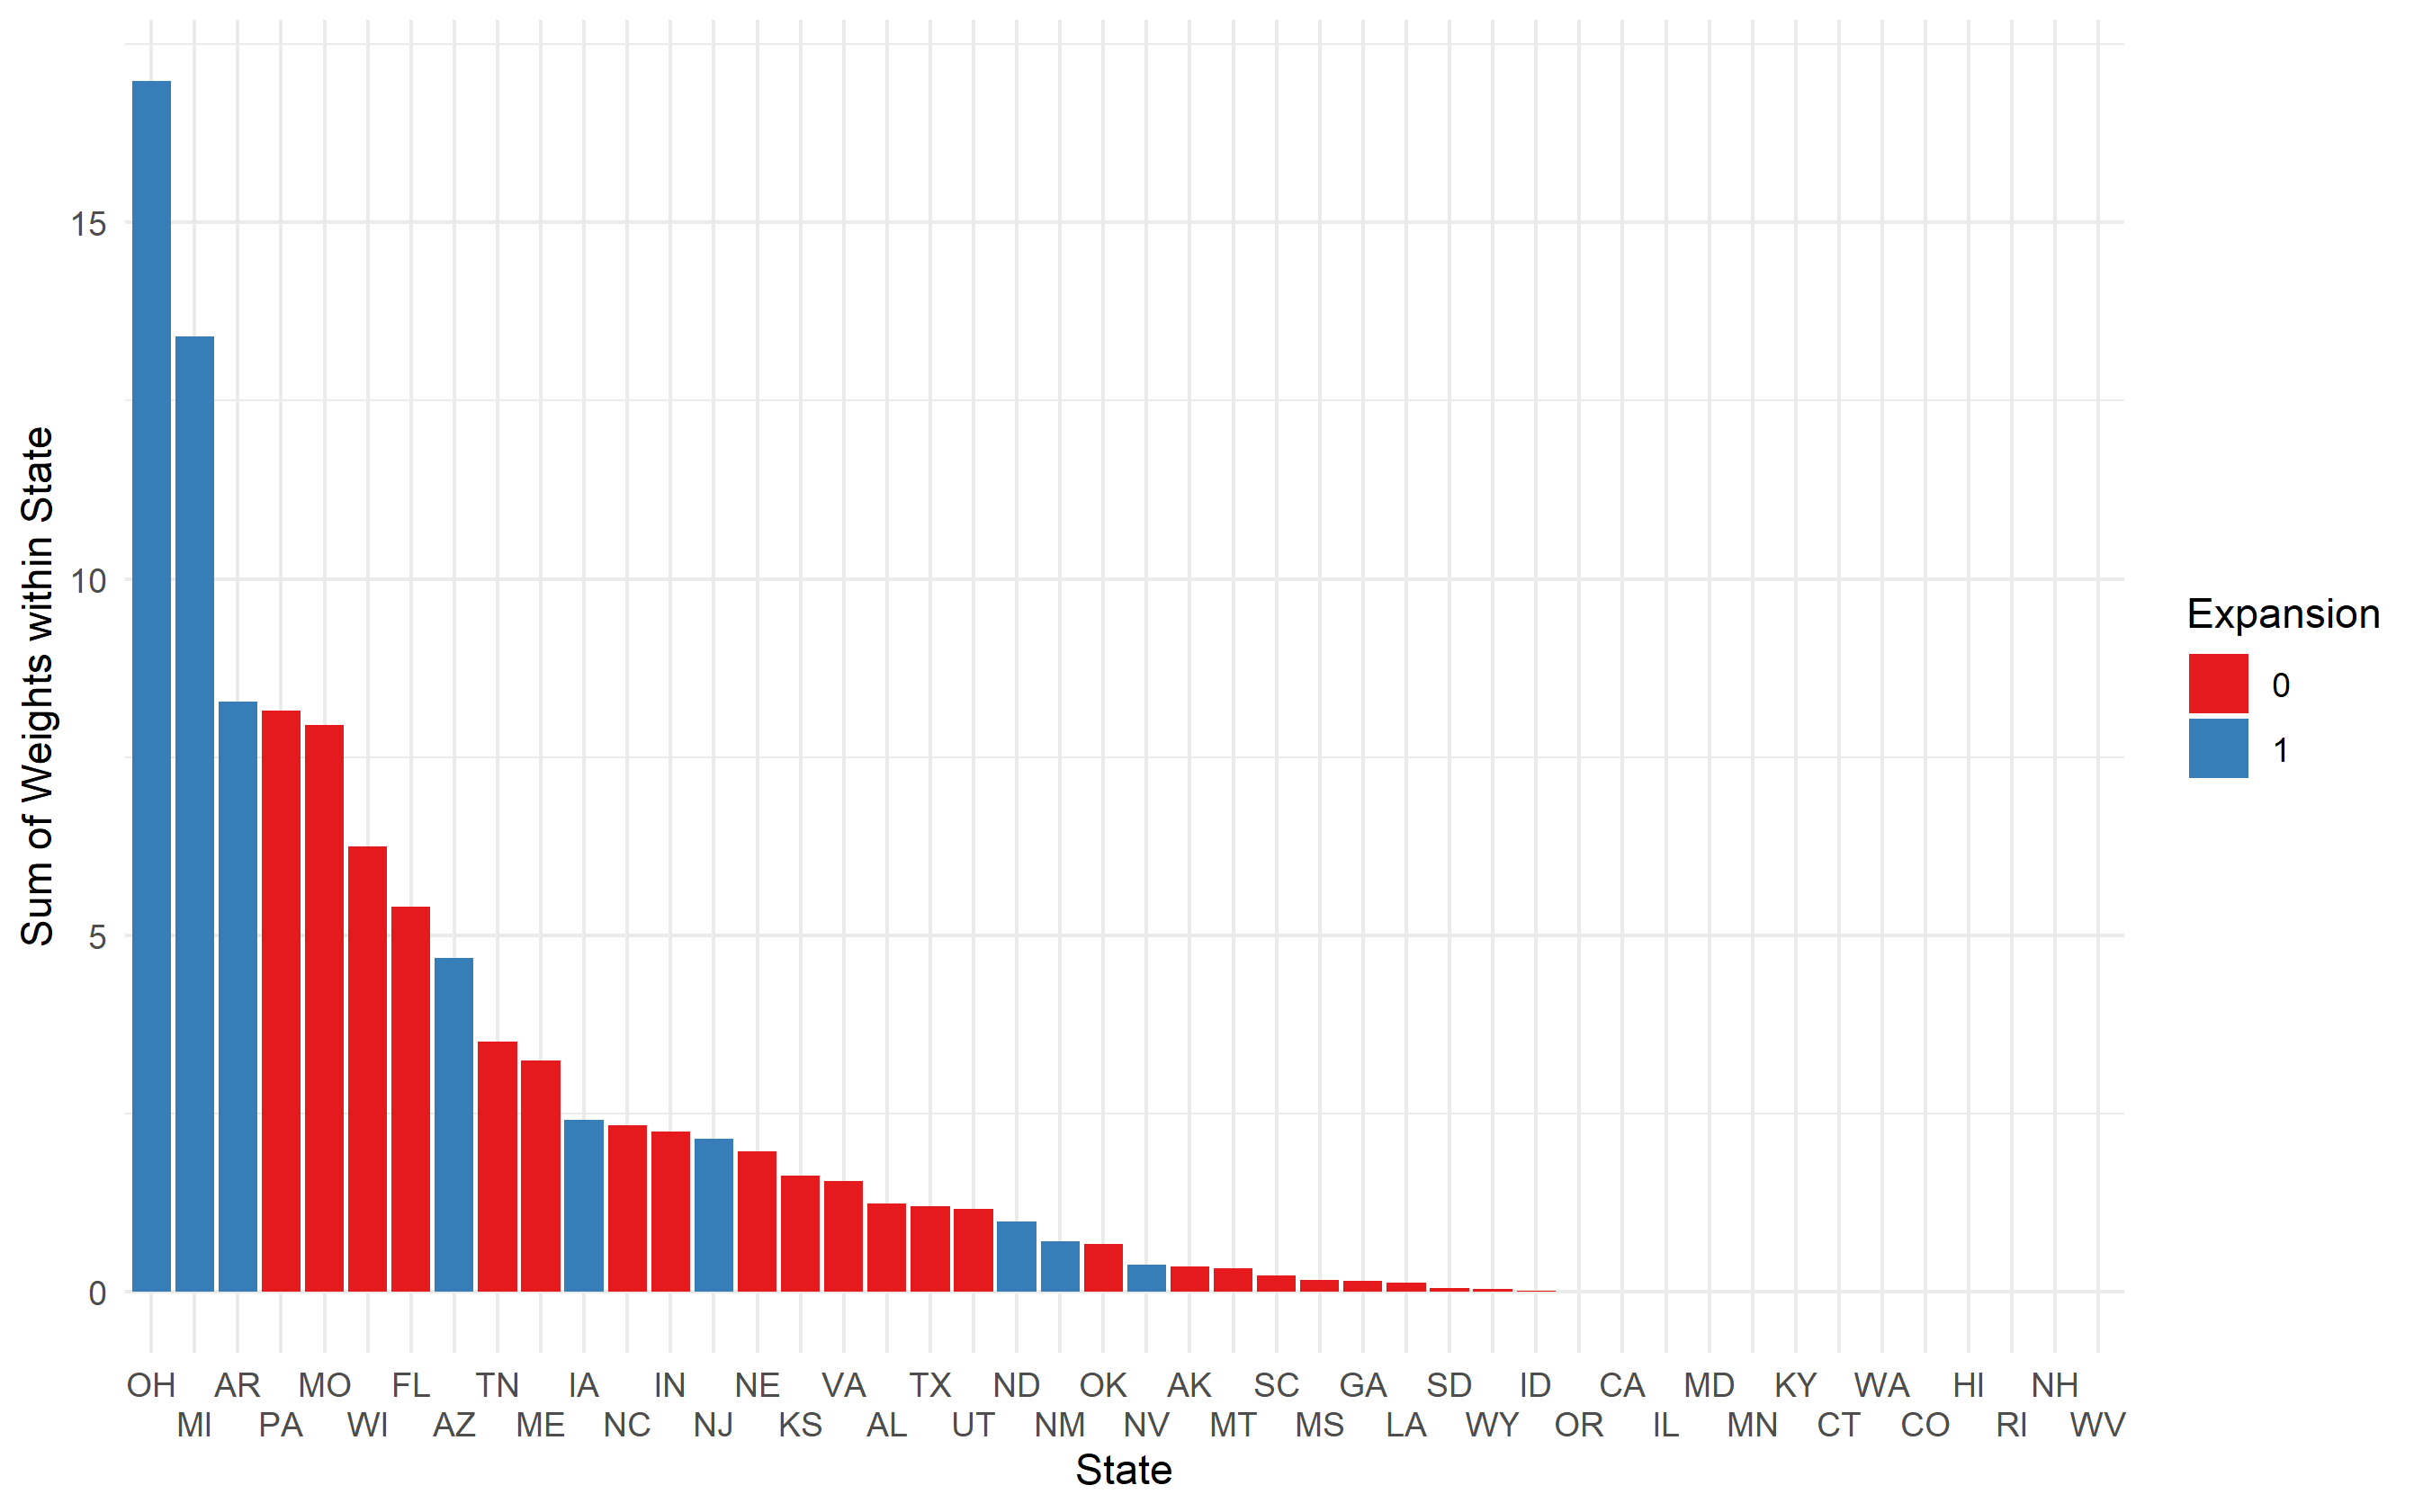
\includegraphics[scale=0.6]{01_Plots/oate-region-c1-a.png}
    \caption{Overlap weights by state}
    \label{oatearea}
\end{center}
\end{figure}

We find similar results to our primary analysis: within the overlap region we estimate a treatment effect -1.64 (-2.40 -0.89) when including all treatment states in our primary analysis, and of -1.81 (-2.47, -1.15) when excluding the early expansion states. The results are quite similar when we use the unadjusted datasets: -1.80 (-2.49, -1.10) on the primary dataset and -1.95 (-2.65, -1.25) when excluding early expansion states. 

We again find a negative difference when comparing an estimate excluding the Republican governance indicators against our primary estimate: specifically, we find that the estimate decreases by -0.96 (-0.81, -1.10) percentage points on the primary dataset and by -0.62 (-0.78, -0.46) percentage points when removing early expansion states. \footnote{Unlike the ETC, this contrast is a function of the differences in the weighted covariates among both the treated and control regions.} Notice that both of these estimates were statistically significant; the confidence intervals increase only slightly when recomputing the entire adjustment when removing each state. Moreover, this negative difference in estimated contrasts holds for each excluded state, regardless of whether or not we conditioned on the adjustment or recalculated it. Additional results are available in Appendix E, Table~\ref{tab:oateconfint} and Table~\ref{tab:oatesensitive}. This result again supports our hypothesis that factors associated with Republican governance drive heterogeneity in the estimated treatment effects.

\section{Discussion}

We estimate that had states that did not expand Medicaid in 2014 expanded their programs, they would have seen a -2.00 (-3.59, -0.40) percentage point change in the adult uninsurance rate. Existing estimates place the ETT between -3 and -6 percentage points; these estimates vary depending on the targeted sub-population of interest, the data used, and the modeling approach (see, eg, \cite{courtemanche2017early}, \cite{kaestner2017effects}, \cite{frean2017premium}). This ETC estimate is therefore closer to zero than these ETT estimates, supporting our original hypothesis that the treatment effect on non-expansion states would be smaller in absolute magnitude. Moreover, we also find suggestive evidence that factors associated with Republican governance may drive this differential. While much of this evidence lay was statistically insignificant, we believe that the consistency of this finding to many of our modeling specifications supports this hypothesis.

We also make several methodological contributions to the literature on balancing weights. First, we extend the synthetic controls literature to estimate the treatment effect on the controls. The key challenge is that we need to predict treatment response rather than the outcome absent treatment. Unlike when estimating the treatment effect on the treated, we cannot use pre-treatment outcomes to conduct variable selection, run placebo tests, or train our model in some other way. This is a fundamentally more difficult problem that requires greater modeling assumptions. Second, we extend the Stable Balancing Weights objective function for use with hierarchical data and covariates measured with error. We modify the criterion to more evenly disperse the weights across states, and the constraint set to to balance on a linear approximation to the true covariate values using regression-calibration techniques (\cite{gleser1992importance}).

Our study's approach also has bearing on estimating and understanding the ETT using a differences-in-differences design when estimating the 2014 effects of Medicaid expansion. If we believe that Republican governance is associated with changes in trends over time, then we need to control for this factor. However, there is likely insufficient overlap to control for these factors without significantly extrapolating from the data. We see that the ETC requires less extrapolation than the ETT with respect to governance, and is therefore in some sense a more estimable quantity.\footnote{We note, however, that the standard parallel trends assumption used to identify the ETT is different to the no unmeasured confounding assumption we made here.} 

More generally our results also suggest that we should not use estimates of the ETT to make inferences about the ETC. Because almost every outcome of interest is largely mediated through increasing the number of insured individuals, and because we have shown that there is likely treatment effect heterogeneity with respect to governance, projecting findings from an estimate of the ETT to the ETC would lead to inaccurate inferences. For example, \cite{miller2019medicaid} study the effect of Medicaid expansion on mortality. Using their estimate of the ETT they project that had all states expanded Medicaid, 15,600 deaths would have been avoided during their study's time-period. If we believe that the ETT were further away from zero than the ETC, we should expect that this projection is an over-estimate. Directly estimating the ETC can therefore also help us better model interesting downstream effects mediated through increasing the number of insured individuals. 

Our results come with three major caveats: (1) we rely on strong parametric assumptions about the outcome model to estimate our causal effect; (2) our identification assumes no unmeasured confounding given the true covariates; (3) our estimated associations between Republican governance and our estimated treatment effect largely fall within our estimated margins of error. 

We conclude by discussing the policy implications of these findings. First, we note that a reduction of adult uninsurance rates by -2.00 percentage points represents approximately a 10 percent reduction in the uninsurance rate among non-expansion states. As observed previously, this estimated treatment effect is closer to zero than corresponding estimates of the ETT (see, eg, \cite{courtemanche2017early}), and we may therefore expect that downstream effects that move away from zero monotonically with the number of uninsured are also closer to zero than estimates of the ETT. Second, we emphasize that the association we find between Republican governance and the estimated treatment effect is only an association: this finding does not imply, for example, that states with more conservative governments in general deliberately make Medicaid enrollment more difficult relative to Democratic states. As \cite{sommers2012understanding} notes, people may be less likely to enroll in Medicaid in conservative states due to social stigma and/or personal beliefs about the welfare state. Regardless of the true cause, to evaluate the policy implications of this finding, we compare this result against Congress's goal in implementing Medicaid expansion in the 2010 ACA, which was to increase health insurance coverage. Measured against this intent, better federal policies should encourage states to make Medicaid enrollment easier, for example, by making enrollment automatic. 

\section{Conclusion}

This is the first study to directly estimate the foregone coverage expansions of Medicaid Expansion on states that did not expand Medicaid in 2014. We also contribute to the methodological literature on synthetic controls by clarifying the assumptions required to use longitudinal data to estimate the ETC rather than the ETT, and to the balancing weights literature more generally by considering the case where we have hierarchical data and covariates measured with error. We estimate that had states that did not expand Medicaid in 2014 done so, they would have seen a -2.00 (-3.59, -0.40) percentage point change in their uninsurance rate. This is substantially closer to zero than existing estimates of the ETT, which range between -3 and -6 percentage points. These estimates are robust to different model specifications and sensitivity analyses examining potential violations of the assumptions of no anticipatory treatment effects and positivity violations.

We also find evidence that Republican governance is associated with estimated effect sizes closer to zero. This association is not statistically significant, but is consistent across our sensitivity analyses. Moreover, it is consistent with existing estimates of the ETT that are also farther away from zero, and the finding that Medicaid take-up rates are lower in Republican-governed states prior to Medicaid expansion in 2014 (\cite{sommers2012understanding}). If the goal of Medicaid expansion is to increase access to insurance for low-income adults, state and federal governments may wish to adopt policies that make Medicaid enrollment automatic, or at least easier.

\section{Acknowledgements}

The authors gratefully acknowledge invaluable advice and comments from Zachary Branson, Dave Choi, Edward Kennedy, Brian Kovak, Akshaya Jha, Lowell Taylor, and Jose Zubizaretta.

\cleardoublepage
\bibliography{research.bib} 

\cleardoublepage

\section{Appendix}

\subsection{Appendix A: Proofs}

We first prove that the asymptotic bias of the SBW estimator under measurement error is equivalent to the asymptotic bias of the OLS estimator under the classical errors-in-variables model. We then prove the unbiasedness of the estimator when balancing on the adjusted covariates when balancing on $\eta_a(W_i) = \mathbb{E}\{X_i \mid W_i, A_i = a\}$ instead of $W_i$. We conclude by noting how our application differs from this stylized introduction; Appendix B provides details on how we applied these ideas for our application.

We begin by outlining the classical errors-in-variables model. Consider the linear model $Y_i^1 = \alpha + X_i^T\beta + \epsilon_i$ and assume we observe covariates $W_i \in \mathbb{R}^d$ which are a vector of mean-unbiased proxies for the true covariate $X_i$; ie $W_i = X_i + v_i$. Assume that $(\epsilon_i, v_i) \sim MVN((0,0), \Sigma_{uu})$ 

$$
\Sigma_{uu} = \begin{pmatrix} 
\Sigma_{\epsilon\epsilon} & 0 \\ 
0 & \Sigma_{vv} 
\end{pmatrix}
$$ 

While often it is more natural to think of $X_i$ as fixed unknown parameters, for motivating purposes, we consider the case where $X_i$ are random. In a slight departure from the classical setup, we also consider the binary treatment indicator $A_i$ and we let $(X_i, W_i \mid A_i = a)$ are iid draws from from $MVN((\mu_a, \mu_a), \Sigma)$ where 

$$
\Sigma = \begin{pmatrix} 
\Sigma_{XX} & \Sigma_{XX} \\ 
\Sigma_{XX} & \Sigma_{WW}  
\end{pmatrix}
$$ 

notice that $\Sigma_{WW} = \Sigma_{XX} + \Sigma_{vv}$.\footnote{For simplicity we have also assumed that $\Sigma_{WW \mid A = 1} = \Sigma_{WW \mid A = 0} = \Sigma_{WW}$ and $\Sigma_{XX \mid A = 1} = \Sigma_{XX \mid A = 0} = \Sigma_{XX}$. This is not a necessary assumption, but helps simplify notation.} By the joint normality of $X_i$ and $W_i$, we know that that 

$$
\mathbb{E}\{X_i \mid W_i, A_i = a\} = \mu_a + \kappa^T(W_i - \mu_a)
$$

where $\kappa = \Sigma_{WW}^{-1}\Sigma_{XX}$.

Let $\psi^1 = \mathbb{E}\{Y_i^1 \mid A_i = 0\}$ and $\mu_y = \mathbb{E}\{Y_i^1\} = \mathbb{E}\{Y_i \mid A_i = 1\}$. From our modeling assumptions we have that

\begin{align*}
    \mathbb{E}\{Y_i^1 \mid X_i = x_i\} &= \alpha + x_i^T\beta \\
    &= \mu_y + (x_i - \mu_1)^T\beta \\
    \implies \psi^1 = \mu_y + (\mu_0 - \mu_1)^T\beta
\end{align*}

Let $\hat{\beta}$ be the OLS estimator of $\beta$ run only on the treatment data. Recall that $\mathbb{E}(\hat{\beta}) = \kappa\beta$ (see, eg, \cite{gleser1992importance}). Consider the estimator $\hat{\psi} = \bar{Y}_1 + (\bar{W}_0 - \bar{W}_1)^T\hat{\beta}$. We have that: 

\begin{align*}
    \hat{\psi} - \psi &= \bar{Y}_1 + (\bar{W}_0 - \bar{W}_1)^T\hat{\beta} - (\mu_y + (\mu_0 - \mu_1)^T\beta) \\
    &= (\bar{Y}_1 - \mu_y) + (\bar{W}_0 - \mu_0)^T\hat{\beta} - (\bar{W}_1 - \mu_1)^T\hat{\beta} + (\mu_0 - \mu_1)^T(\hat{\beta} - \beta) \\
    \hat{\psi} - \psi &\to (\mu_0 - \mu_1)^T(\kappa - I_d)\beta
\end{align*}

The final result holds because in the second line, the first term is simply the estimation error from a sample average and has expectation zero. The second term is the product of the estimation error from a sample average and $\hat{\beta}$; this also has expectation zero because $\bar{X}_0$ is estimated on a different part of the sample than $\hat{\beta}$, so these errors are independent. The third term is more complicated because the estimation error of $\mu_1$ is not independent of $\hat{\beta}$ since they are typically estimated using the same sample. However, we know that the estimation error converges in probability to zero and $\hat{\beta} \to \kappa\beta$; therefore, by Slutsky's Theorem, this term also converges in probability to zero, and we are left with the asymptotic bias noted above. 

We now consider the SBW estimator that sets $\delta = 0$ and show that this estimator has the same asymptotic bias. More formally, define the SBW estimator as:

$$
\arg\min_{\gamma \in \Gamma} \gamma_i^2
$$

$$
\Gamma := \{\gamma: W_1^T\gamma = \bar{W}_0, \gamma_i > 0, \gamma^T1 = 1\}
$$

We first consider the error of our estimator:

\begin{align*}
    \hat{\psi} - \psi &= \sum_{i: A_i = 0}w_iY_i - (\alpha + \mu_0^T\beta) \\
    &= \sum_i \gamma_i(\alpha + X_i^T\beta + \epsilon_i) - (\alpha + \bar{W}_0^T\beta + (\mu_0 - \bar{W}_0)^T\beta) \\
    &= \sum_i (\gamma_i(W_i - v_i)^T\beta + \gamma_i\epsilon_i) - \bar{W}_0^T\beta + (\mu_0 - \bar{W}_0)^T\beta \\
    &= -\sum_{i: A_i = 1}\gamma_iv_i^T\beta + \sum_{i: A_i = 1}\gamma_i\epsilon_i  + (\mu_0 - \bar{W}_0)^T\beta
\end{align*}

Conditioning on $W_i$, we can take expectations over $X_i$, and see that the second term has expectation zero (noting that the weights, conditional on $W_i$, are independent of these errors). The third term is simply the scaled sum of mean zero estimation error and therefore has expectation zero. We conclude by considering the first term and again take expectations over $X_i$ conditional on $W_i$: 

\begin{align*}
    \sum_{i: A_i = 1} \gamma_i\mathbb{E}\{X_i - W_i \mid W_i\}^T\beta &= \sum_{i: A_i = 1} \gamma_i (\mu_1 + \kappa^T(W_i - \mu_1))^T\beta - \sum_{i: A_i = 1}\gamma_i W_i^T\beta \\
    &= (\mu_1 + \kappa^T(\bar{W}_0 - \mu_1))^T\beta - \bar{W}_0^T\beta \\
    &= (\kappa^T(\bar{W}_0 - \mu_1))^T\beta - (\bar{W}_0 - \mu_1)^T\beta  \\
    &= (\bar{W}_0 - \mu_1)^T(\kappa - I_d)\beta \\
    &= (\mu_0 - \mu_1)^T(\kappa - I_d)\beta + (\bar{W}_0 - \mu_0)^T(\kappa - I_d)\beta \\
\end{align*}

Taking the expectation over $W_i$, the second term is a scaled sum of mean zero estimation error and has expectation zero. We therefore see that the asymptotic bias of the SBW estimator is equivalent to the OLS estimator.

We conclude by showing the unbiasedness of the estimator that reweights $\eta_1(W_i)$ rather than $W_i$. We make the simplifying assumptions that $\eta_a(W_i)$ and $\mu_0$ are known, and that there is no model error on $Y_i$. Assume that $\sum_{i: A_i = 1}\gamma_i\eta_1(W_i) = \mu_0$. By linearity, we know that

$$
(Y_i^1 \mid A_i = a) = \alpha + \eta_a(W_i)^T\beta + (X_i - \eta_a(W_i))^T\beta
$$

We then have that:

\begin{align*}
    \hat{\psi} - \psi &= \sum_{i: A_i = 1}\gamma_iY_i - (\alpha + \mu_0^T\beta) \\
    &= \sum_{i: A_i = 1}\gamma_i\alpha + \sum_{i: A_i = 1}\gamma_i\eta_1(W_i)^T\beta + \sum_{i: A_i = 1}\gamma_i(X_i - \eta_0(W_i))^T\beta - (\alpha + \mu_0^T\beta) \\
    &= \sum_{i: A_i = 1}\gamma_i(X_i - \eta_1(W_i))^T\beta
\end{align*}

Since the weights are independent of the errors $X_i - \eta_1(W_i)$, and $\eta_1(W_i)$ is an unbiased estimate of $X_i$, these terms are both mean zero when taking expectations over $X_i$. Notice that even though we have assumed no model error, this estimator still has variance, conditional on $W_i$, equal to

$$
\sum_{i: A_i = 0} \gamma_i^2\beta^TCov(X_i \mid W_i)\beta
$$

where, assuming that $(X_i, W_i)$ are jointly normally distributed, $Cov(X_i \mid W_i) = \Sigma_{XX} - \Sigma_{XX}\Sigma_{WW}^{-1}\Sigma_{XX}$. This shows that the variance of this estimator is higher than if we knew the true $X_i$, even if we knew $\eta_a(W_i)$, unless $\Sigma_{WW} = \Sigma_{XX}$ (ie there is no error in $X_i$). 

We conclude by noting several key departures in our applied setting to the framework we presented above: first, our causal parameter is a sample-average estimand, and we therefore we view $X_i$ as fixed underlying parameters.\footnote{In this case the error terms we derived above lead to a finite-sample bias rather than contributing the estimator's variance.} Second, we don't know $\eta_a(W_i)$ and instead approximate it using an estimate of $\Sigma_{vv}$ using auxillary data and an estimate of $\Sigma_{WW}$ from the observed data. Finally, we do not believe that $X_i$ is linear in $W_i$; however, we can view this adjustment as the best linear predictor of $X_i$. An extensive literature exists on regression calibration methods that considers the theory of these approximations under different conditions (see, eg, \cite{gleser1992importance}, \cite{carroll2006measurement}). Further consideration of these issues is beyond the scope of this paper.

\subsection{Appendix B: Calibration Details}

We now discuss how we estimate $\eta_a(W_i)$. We first outline the more conventional adjustment outlined in \cite{carroll2006measurement}, and then we explain our preferred departures from this framework. In either case we begin by estimating the covariance matrix $\Sigma_{UU, sc}$, the sampling variability for each CPUMA using the individual replicate survey weights to generate $b = 80$ additional CPUMA-level datasets. We then estimate the covariance matrix of the measurement errors using:

$$
\hat{\Sigma}_{vv, sc} = \frac{4}{80}\sum_{b=1}^{80}(X_{sc}^B - \bar{X}_{sc})(X_{b, sc} - \bar{X}_{sc})^T
$$

where the $4$ in the numerator comes from the process used to generate the replicate survey weights. Let $\hat{\Sigma}_{vv \mid A = a} = N_a^{-1}\sum_{s, c: A_s = a} (W_{sc} - \bar{W})(W_{sc} - \bar{W})^T$. This estimator is calculated on the original observed dataset. We then estimate $\Sigma_{XX \mid A = a}$ using:

$$
\hat{\Sigma}_{XX \mid A = a} = \hat{\Sigma}_{WW \mid A = a} - N_a^{-1}\sum_{s, c: A_s = a} \hat{\Sigma}_{UU, sc}
$$

Define

$$
\hat{\kappa}_a = (\hat{\Sigma}_{WW \mid A = a})^{-1}(\hat{\Sigma}_{XX \mid A = a})
$$

We can think of this as a matrix of estimated coefficients of a linear regressions of the (unobserved) matrix $X_{sc}$ on (observed) matrix $W_{sc}$. We can estimate $X_{sc}$ as

$$
\hat{\eta}_a(W_{sc}) = \bar{W}_a + \hat{\kappa}_a^T(W_{sc} - \bar{W}_a)
$$

where $\bar{W}_a = N_a^{-1}\sum_{i: A_i = a} W_{sc}$. This approximately aligns with the adjustments suggested by \cite{carroll2006measurement} and \cite{gleser1992importance}. However, in our setting we have additional access to information about a substantial source of heterogeneity in the measurement error: in particular, regions with large populations are estimated quite precisely, while regions with small populations are estimated much less precisely. This is because the survey is a one-percent sample across all regions. Moreover, for a given CPUMA, some covariates are measured using three years of data, and others only one. However, using the conventional regression calibration approach will adjust precisely estimated covariates to imprecisely estimated covariates in a similar way. 

Our preferred estimators therefore use an alternative approach where we model an individual-level $\Sigma_{vv, sc}$ as a function of the sample sizes used to estimate each covariate. In particular, let $s_{sc}$ be the d-dimensional vector of the sample sizes used to estimate each covariate value for a given CPUMA. Let $S_{sc} = \sqrt{s_{sc}}\sqrt{s_{sc}}^T$. We assume that $\sqrt{s_{sc}}v_{sc} \sim N(0, \Sigma_{vv}^a)$. We then know that $\Sigma_{vv, sc}^m = \Sigma_{vv}^a \oslash S_{sc}$. We add the superscript $m$ to distinguish that is a modeled covariance matrix.

To estimate these matrices, we pool our initial estimates of the CPUMA-level covariance matrices ($\hat{\Sigma}_{vv, sc}$) to generate $\hat{\Sigma}_{vv}^a = N_a^{-1}\sum_{s, c: A_s = a} S_{sc} \circ \Sigma_{vv, sc}$. We then estimate $\hat{\Sigma}_{vv, sc}^m = \hat{\Sigma}_{vv}^a \oslash S_{sc}$. From this we estimate $\hat{\Sigma}_{XX \mid A = a} = \hat{\Sigma}_{WW \mid A = a} - N_a^{-1}\sum_{s, c: A_s = a}\hat{\Sigma}_{vv, sc}^a$. Finally, we calculate $\hat{\kappa}_{sc} = (\hat{\Sigma}_{XX \mid A = a} + \hat{\Sigma}_{vv, sc}^m)^{-1}\hat{\Sigma}_{XX \mid A = a}$, which we use to estimate $\hat{\eta}_a(W_{sc})$. 

The benefit of this estimator is that we account for unit-level heterogeneity in the measurement error. Specifically, this adjustment should primarily affect outlying values of imprecisely estimated covariates, while leaving precisely estimated covariates largely unchanged. Moreover, we are able to use the full efficiency of using all units in the modeling. The disadvantage is that, as shown in Appendix~\ref{sec:appendixsumstat}, this adjustment, compared to the conventional approach, is more likely to lead to extreme values that fall outside of the support of the original data, or of the possible values entirely. A second cost of this procedure is that this aggregation models all differences as a function of the sample sizes, and averages over any potential heterogeneity due to heteroskedasticity (ie the measurement error covariance matrix changes depending on the true value of $X_{sc}$). However, in practice we find that either adjustment yields quite similar results (see Appendix~\ref{ssec:allresults}).

\subsection{Appendix C: Summary Statistics}
\label{sec:appendixsumstat}

Table~\ref{tab:summarytab1}, Table~\ref{tab:summarytab2}, and Table~\ref{tab:summarytab3} display univariate summary statistics from the primary dataset. We display the mean, interquartile range, and the range (as defined by the maximum value minus the minimum value) for the unadjusted dataset (sigma\_zero), the preferred adjustment (sigma\_uu\_i), and the secondary adjustment (sigma\_uu\_avg). We see that in general the secondary adjustment reduces the variability in the data. The preferred adjustment reduces the interquartile range, but increases the overall variability (as measured by the range) by causing extreme values for particular CPUMAs. However, these extreme values are quite rare; we display the overall number of CPUMAs whose adjusted values fall outside of the range of the unadjusted data in Table~\ref{tab:extreme1} and Table~\ref{tab:extreme2}. Note that for our ETT estimates, we only use the adjustments on the treatment data, while we use both for the OATE estimates. As a reminder there are 414 control group CPUMAs and 515 treatment group CPUMAs.

We also calculate these adjustments when excluding the early expansion states and leaving out each state one at a time from the primary dataset and from the early expansion states excluded dataset; these results are available on request. 

\begin{table}[ht]
\centering
\begin{tabular}{rllll}
  \toprule
Treat & Variable & sigma\_zero & sigma\_uu\_avg & sigma\_uu\_i \\ 
  \midrule
0 & age\_cat2\_19\_29\_pct & (24.8, 5.5, 48.7) & (24.8, 5.4, 47.8) & (24.8, 5.4, 66) \\ 
  1 & age\_cat2\_19\_29\_pct & (24.5, 6, 30.9) & (24.5, 5.9, 29) & (24.5, 5.9, 29) \\ 
  0 & age\_cat2\_30\_39\_pct & (20.6, 2.6, 18.4) & (20.6, 2.5, 17.2) & (20.4, 2.6, 89) \\ 
  1 & age\_cat2\_30\_39\_pct & (20.9, 3.4, 20.9) & (20.9, 3.2, 19.4) & (20.9, 3.1, 41.3) \\ 
  0 & age\_cat2\_40\_49\_pct & (22, 2.5, 19.5) & (22, 2.3, 18.5) & (22.2, 2.4, 119.8) \\ 
  1 & age\_cat2\_40\_49\_pct & (22.2, 2.5, 15.4) & (22.2, 2.3, 13.8) & (22.3, 2.3, 53.6) \\ 
  0 & avg\_adult\_hh\_ratio & (139.7, 18.7, 156.8) & (139.7, 19, 154) & (139.5, 19.1, 202.9) \\ 
  1 & avg\_adult\_hh\_ratio & (150.8, 27.1, 174.3) & (150.8, 27.1, 173.3) & (150.8, 27, 173.8) \\ 
  0 & citizenship\_pct & (93.6, 5.9, 39.8) & (93.6, 5.9, 39.3) & (93.6, 5.8, 39.7) \\ 
  1 & citizenship\_pct & (90, 11.8, 57.1) & (90, 11.7, 55.7) & (90, 11.8, 55.4) \\ 
  0 & disability\_pct & (11.9, 5, 22.1) & (11.9, 4.8, 20.7) & (11.9, 4.9, 20.5) \\ 
  1 & disability\_pct & (10.5, 5.3, 28.6) & (10.5, 5.4, 27.2) & (10.4, 5.2, 26.7) \\ 
  0 & educ\_hs\_degree\_pct & (29.6, 8.8, 42.7) & (29.6, 8.8, 41.2) & (29.8, 8.8, 136.5) \\ 
  1 & educ\_hs\_degree\_pct & (26.3, 10.6, 43.2) & (26.3, 10.7, 41.9) & (26.3, 10.5, 41.8) \\ 
  0 & educ\_less\_than\_hs\_pct & (11.8, 7.1, 30) & (11.8, 7, 30.2) & (11.6, 7, 90.3) \\ 
  1 & educ\_less\_than\_hs\_pct & (11.4, 7.6, 45.3) & (11.4, 7.3, 44.6) & (11.3, 7.4, 47.3) \\ 
  0 & educ\_some\_college\_pct & (33.8, 5.6, 42.9) & (33.8, 5.1, 42.3) & (33.9, 5, 65.8) \\ 
  1 & educ\_some\_college\_pct & (33.5, 7.8, 34.2) & (33.5, 7.3, 32.9) & (33.5, 7.4, 40.1) \\ 
  0 & female\_pct & (50.5, 1.6, 15.8) & (50.5, 1.5, 15.1) & (50.5, 1.5, 14.9) \\ 
  1 & female\_pct & (50.1, 1.6, 15.4) & (50.1, 1.5, 14.2) & (50.1, 1.4, 14.2) \\ 
  0 & foreign\_born\_pct & (10.5, 8.8, 63.2) & (10.5, 8.9, 62.7) & (10.4, 8.8, 96.5) \\ 
  1 & foreign\_born\_pct & (18, 22.2, 76) & (18, 22.2, 75.3) & (18, 22.2, 75.2) \\ 
  0 & hins\_unins\_pct\_2011 & (22.7, 10.5, 51.4) & (22.7, 9.2, 50.3) & (26.1, 9.8, 2066.1) \\ 
  1 & hins\_unins\_pct\_2011 & (19.6, 11.2, 59) & (19.6, 10.8, 52.3) & (19.4, 10.9, 154.1) \\ 
  0 & hins\_unins\_pct\_2012 & (22.4, 9.3, 49.5) & (22.4, 9.1, 47.8) & (22.2, 9.4, 178.3) \\ 
  1 & hins\_unins\_pct\_2012 & (19.4, 9.8, 50.6) & (19.4, 10.1, 50.1) & (19.3, 10.1, 96.9) \\ 
  0 & hins\_unins\_pct\_2013 & (22, 10.1, 50.1) & (22, 9.4, 49.2) & (19.4, 9.4, 1580.6) \\ 
  1 & hins\_unins\_pct\_2013 & (19, 11.1, 49.9) & (19, 10.4, 48.6) & (19.2, 10.5, 135.3) \\ 
   \bottomrule
\end{tabular}
    \caption{Univariate summary statistics (1)}
    \label{tab:summarytab1}
\end{table}

\begin{table}[ht]
\centering
\begin{tabular}{rllll}
  \toprule
Treat & Variable & sigma\_zero & sigma\_uu\_avg & sigma\_uu\_i \\ 
  \midrule
  0 & hispanic\_pct & (11.4, 10.2, 93.9) & (11.4, 10.2, 93.8) & (11.4, 10.2, 93.8) \\ 
  1 & hispanic\_pct & (15.8, 17.7, 97.2) & (15.8, 17.7, 97) & (15.8, 17.7, 97) \\ 
  0 & inc\_pov2\_138\_pct & (22, 8.8, 42.8) & (22, 8.7, 41.8) & (22, 8.7, 47.2) \\ 
  1 & inc\_pov2\_138\_pct & (19.9, 11.9, 45.6) & (19.9, 11.7, 43.9) & (20, 11.8, 50.2) \\ 
  0 & inc\_pov2\_139\_299\_pct & (27.4, 5.1, 27.9) & (27.4, 4.8, 26.7) & (28.4, 5, 611.1) \\ 
  1 & inc\_pov2\_139\_299\_pct & (24.9, 8.4, 34.2) & (24.9, 7.8, 34.2) & (24.9, 7.9, 34.2) \\ 
  0 & inc\_pov2\_300\_499\_pct & (24.2, 4.8, 21) & (24.2, 4.6, 18.4) & (22.8, 4.6, 819.1) \\ 
  1 & inc\_pov2\_300\_499\_pct & (23.6, 5.5, 23) & (23.6, 4.8, 22.1) & (23.6, 5, 25) \\ 
  0 & inc\_pov2\_500\_plus\_pct & (23.7, 9.9, 51.9) & (23.7, 9.7, 52.1) & (24.1, 9.8, 221.6) \\ 
  1 & inc\_pov2\_500\_plus\_pct & (29.3, 18.4, 69.1) & (29.3, 18.5, 68) & (29.3, 18.4, 68) \\ 
  0 & married\_pct & (51.5, 9.1, 59.7) & (51.5, 9.1, 59.5) & (51.2, 9.2, 198.5) \\ 
  1 & married\_pct & (50.7, 9.4, 45.1) & (50.7, 9.1, 44.3) & (50.7, 9, 44.2) \\ 
  0 & missing\_children\_pct & (13.7, 7.4, 36.2) & (13.7, 7.3, 35.6) & (13.7, 7.3, 59.6) \\ 
  1 & missing\_children\_pct & (10.5, 6.6, 41) & (10.5, 6.6, 40.5) & (10.5, 6.6, 40.7) \\ 
  0 & one\_child\_pct & (10.4, 2.5, 13) & (10.4, 2.1, 12.4) & (10.9, 2.3, 291.9) \\ 
  1 & one\_child\_pct & (11.1, 3.1, 14.3) & (11.1, 2.9, 12.5) & (11.1, 2.8, 12.3) \\ 
  0 & pop\_growth\_2012 & (100.4, 2.3, 29.4) & (100.4, 2.1, 12.4) & (109.1, 2.4, 5163.5) \\ 
  1 & pop\_growth\_2012 & (100.2, 3.1, 27.8) & (100.2, 2.2, 15.4) & (98.1, 2.3, 1217.6) \\ 
  0 & pop\_growth\_2013 & (100.3, 2.6, 20.5) & (100.3, 1.7, 13.1) & (107.6, 2, 4348.5) \\ 
  1 & pop\_growth\_2013 & (100.3, 3.1, 30.1) & (100.3, 2.3, 12.4) & (98, 2.5, 1265.4) \\ 
  0 & race\_white\_pct & (77.8, 22.2, 90.5) & (77.8, 22.1, 90.4) & (77.8, 22, 90.2) \\ 
  1 & race\_white\_pct & (73.9, 25.4, 91.9) & (73.9, 25.5, 91.8) & (73.9, 25.6, 91.7) \\ 
  0 & repub\_gov & (95.9, 0, 100) & (95.9, 0, 100) & (95.9, 0, 100) \\ 
  1 & repub\_gov & (30.9, 100, 100) & (30.9, 100, 100) & (30.9, 100, 100) \\ 
  0 & repub\_lower\_control & (98.8, 0, 100) & (98.8, 0, 100) & (98.8, 0, 100) \\ 
  1 & repub\_lower\_control & (23.9, 0, 100) & (23.9, 0, 100) & (23.9, 0, 100) \\ 
  0 & repub\_total\_control & (94.7, 0, 100) & (94.7, 0, 100) & (94.7, 0, 100) \\ 
  1 & repub\_total\_control & (21, 0, 100) & (21, 0, 100) & (21, 0, 100) \\
   \bottomrule
\end{tabular}
    \caption{Univariate summary statistics (2)}
    \label{tab:summarytab2}
\end{table}

\begin{table}[ht]
\centering
\begin{tabular}{rllll}
  \toprule
Treat & Variable & sigma\_zero & sigma\_uu\_avg & sigma\_uu\_i \\ 
  \midrule
  0 & student\_pct & (11.5, 3.9, 41) & (11.5, 3.8, 41.3) & (11.6, 3.8, 92.7) \\ 
  1 & student\_pct & (11.7, 3.4, 29.5) & (11.7, 3.4, 28) & (11.7, 3.4, 28.1) \\ 
  0 & three\_plus\_child\_pct & (5.2, 2.2, 25.3) & (5.2, 2.2, 23.2) & (5.4, 2.2, 94.7) \\ 
  1 & three\_plus\_child\_pct & (5.2, 2, 14.1) & (5.2, 1.7, 13.3) & (5.2, 1.7, 13.5) \\ 
  0 & two\_child\_pct & (8.9, 2.8, 15) & (8.9, 2.5, 15.1) & (8.5, 2.5, 278.8) \\ 
  1 & two\_child\_pct & (9.7, 3.5, 15) & (9.7, 3.2, 13.6) & (9.7, 3.2, 16.1) \\ 
  0 & unemployed\_pct\_2011 & (9.4, 4.6, 21.7) & (9.4, 4.1, 18.7) & (9.7, 3.9, 189.1) \\ 
  1 & unemployed\_pct\_2011 & (10.2, 4.6, 25.5) & (10.2, 4, 22.6) & (10.1, 3.9, 89.9) \\ 
  0 & unemployed\_pct\_2012 & (8.8, 4.2, 22.4) & (8.8, 3.6, 18.7) & (9.4, 3.6, 370.1) \\ 
  1 & unemployed\_pct\_2012 & (9.4, 4.5, 28.3) & (9.4, 4.3, 23.6) & (9.3, 4.4, 23.7) \\ 
  0 & unemployed\_pct\_2013 & (8, 3.7, 19) & (8, 3.4, 17.6) & (7.4, 3.4, 319.9) \\ 
  1 & unemployed\_pct\_2013 & (8.4, 3.7, 23.4) & (8.4, 3.5, 20.6) & (8.3, 3.5, 20.5) \\ 
  0 & urban\_pct & (74.6, 39.2, 85.7) & (74.6, 39.2, 85.7) & (74.6, 39.2, 85.7) \\ 
  1 & urban\_pct & (82.7, 31.5, 91.3) & (82.7, 31.5, 91.3) & (82.7, 31.5, 91.3) \\ 
   \bottomrule
\end{tabular}
    \caption{Univariate summary statistics (3)}
    \label{tab:summarytab3}
\end{table}

Table~\ref{tab:extreme1} and Table~\ref{tab:extreme2} display the frequency that the adjusted covariates fell outside of the support of the unadjusted dataset for the (control, treatment) groups. We see that that frequency is higher for our preferred adjustment (sigma\_uu\_i) than the secondary adjustment (sigma\_uu\_avg), though the counts are low in either case. The counts are also slightly higher in the control group than the treated group; this may be a function of the smaller number of CPUMAs for the control versus the treated group $(N_0 = 414; N_1 = 515)$.

\begin{table}[ht]
\centering
\begin{tabular}{lll}
  \toprule
Variable & sigma\_uu\_avg & sigma\_uu\_i \\ 
  \midrule
age\_cat2\_19\_29\_pct & (0, 0) & (1, 0) \\ 
  age\_cat2\_30\_39\_pct & (0, 0) & (1, 1) \\ 
  age\_cat2\_40\_49\_pct & (0, 0) & (2, 1) \\ 
  avg\_adult\_hh\_ratio & (0, 0) & (1, 0) \\ 
  citizenship\_pct & (1, 0) & (3, 0) \\ 
  disability\_pct & (0, 2) & (0, 2) \\ 
  educ\_hs\_degree\_pct & (0, 0) & (1, 0) \\ 
  educ\_less\_than\_hs\_pct & (2, 1) & (3, 2) \\ 
  educ\_some\_college\_pct & (0, 0) & (1, 1) \\ 
  female\_pct & (0, 0) & (0, 0) \\ 
  foreign\_born\_pct & (0, 0) & (1, 1) \\ 
  hins\_unins\_pct\_2011 & (0, 0) & (6, 1) \\ 
  hins\_unins\_pct\_2012 & (0, 1) & (1, 1) \\ 
  hins\_unins\_pct\_2013 & (1, 1) & (4, 1) \\ 
  hispanic\_pct & (1, 0) & (1, 0) \\ 
  inc\_pov2\_138\_pct & (2, 1) & (3, 2) \\ 
  inc\_pov2\_139\_299\_pct & (1, 1) & (6, 1) \\ 
  inc\_pov2\_300\_499\_pct & (0, 0) & (5, 1) \\ 
  inc\_pov2\_500\_plus\_pct & (2, 0) & (4, 0) \\ 
   \bottomrule
\end{tabular}
    \caption{Extreme covariate adjustments (1)}
    \label{tab:extreme1}
\end{table}

\begin{table}[ht]
\centering
\begin{tabular}{lll}
  \toprule
Variable & sigma\_uu\_avg & sigma\_uu\_i \\ 
  \midrule
  married\_pct & (1, 0) & (3, 0) \\ 
  missing\_children\_pct & (1, 0) & (2, 1) \\ 
  one\_child\_pct & (0, 0) & (3, 0) \\ 
  pop\_growth\_2012 & (0, 0) & (11, 6) \\ 
  pop\_growth\_2013 & (0, 0) & (11, 4) \\ 
  race\_white\_pct & (1, 1) & (1, 1) \\ 
  student\_pct & (1, 0) & (3, 0) \\ 
  three\_plus\_child\_pct & (2, 0) & (5, 2) \\ 
  two\_child\_pct & (2, 1) & (5, 2) \\ 
  unemployed\_pct\_2011 & (0, 0) & (3, 1) \\ 
  unemployed\_pct\_2012 & (0, 0) & (5, 0) \\ 
  unemployed\_pct\_2013 & (0, 0) & (3, 0) \\ 
   \bottomrule
\end{tabular}
    \caption{Extreme covariate adjustments (2)}
    \label{tab:extreme2}
\end{table}

Figure~\ref{fig:corrmatrix} displays the Pearson's correlation coefficients for the bivariate relationships between the covariates on the unadjusted dataset. The relationships are quite similar when using the ``sigma\_uu\_avg'' adjustment, but change quite a bit do to the extreme values on the third adjustment. These results are available on request.

\begin{figure}[]
\begin{center}
    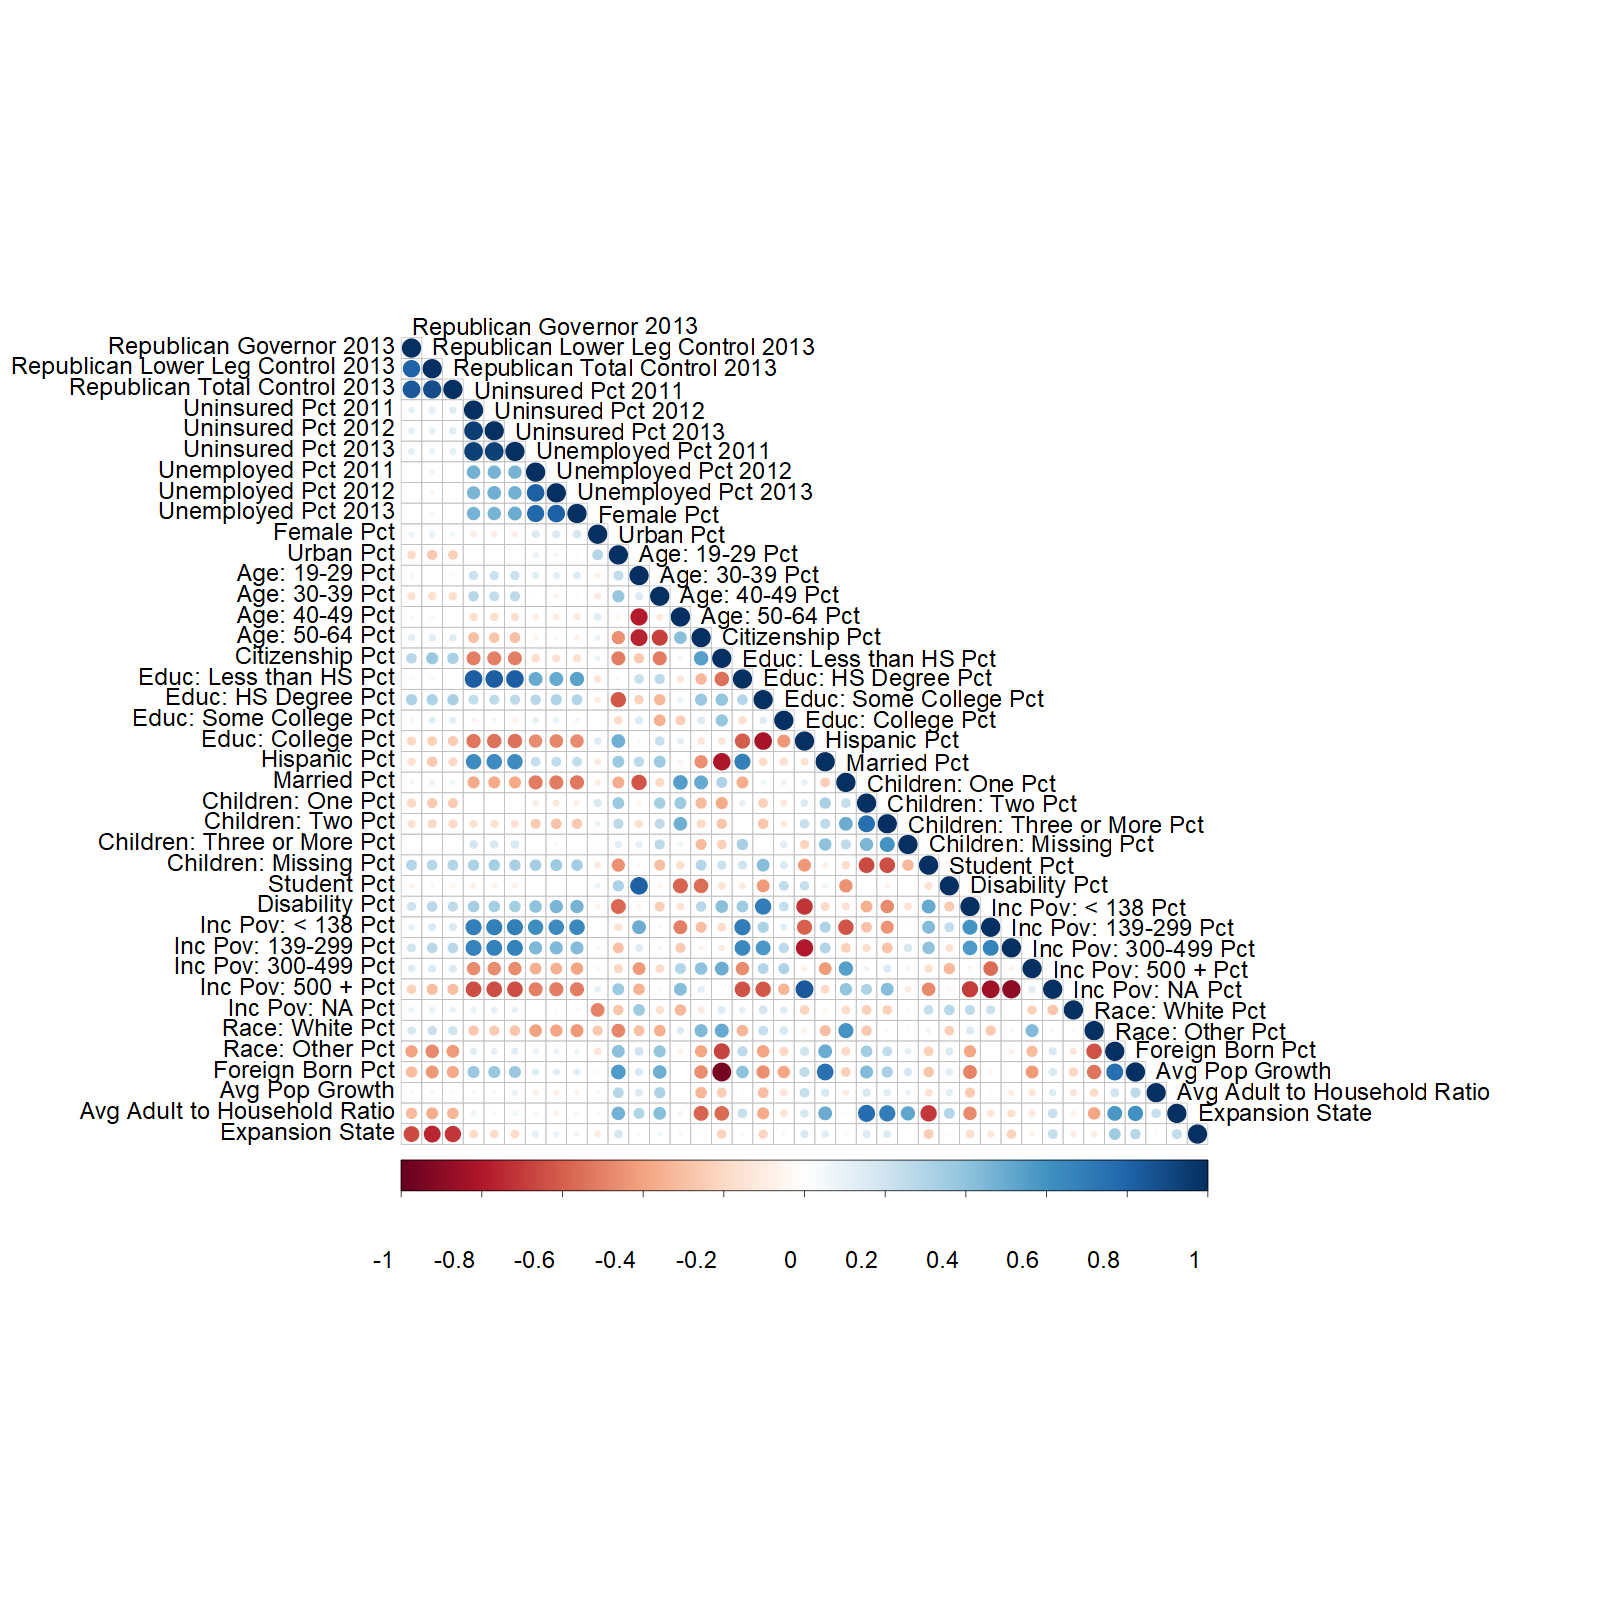
\includegraphics[scale=0.6]{01_Plots/correlation-plot-c1-sigma-zero.png}
    \caption{Correlation matrix (unadjusted covariates)}
    \label{fig:corrmatrix}
\end{center}
\end{figure}

\subsection{Appendix D: Weight Diagnostics}
\label{ssec:balancetables}

Table~\ref{tab:baltab1} and Table~\ref{tab:baltab2} display the differences between the population-weighted mean covariate values of the non-expansion region and the weighted mean of the expansion region for our primary dataset and with the early expansion states excluded (calculated using our covariate adjustments). The weights presented here are from the H-SBW estimator. The values under each column of ``Primary'' and ``Early Excluded'' are in the following format: (unweighted difference, weighted difference). Additional results are available on request.

\begin{table}[ht]
\centering
\begin{tabular}{lll}
  \toprule
Variables & Primary & Early Excluded \\ 
  \midrule
age\_cat2\_19\_29\_pct & (0.51, 0.50) & (0.80, -0.11) \\ 
  age\_cat2\_30\_39\_pct & (0.23, 0.42) & (0.57, -0.14) \\ 
  age\_cat2\_40\_49\_pct & (-0.10, 0.50) & (0.19, 0.65) \\ 
  avg\_adult\_hh\_ratio & (-10.11, -0.15) & (-2.18, -0.25) \\ 
  citizenship\_pct & (2.19, 2.00) & (-1.16, 1.69) \\ 
  disability\_pct & (1.01, -0.52) & (-0.25, -0.43) \\ 
  educ\_hs\_degree\_pct & (2.38, -1.54) & (0.04, -0.54) \\ 
  educ\_less\_than\_hs\_pct & (0.74, -1.32) & (1.58, -0.78) \\ 
  educ\_some\_college\_pct & (-0.01, -0.75) & (-0.69, -0.83) \\ 
  female\_pct & (0.34, 0.72) & (0.24, 1.00) \\ 
  foreign\_born\_pct & (-5.26, -2.00) & (1.29, -2.00) \\ 
  hins\_unins\_pct\_2011 & (4.37, -0.05) & (4.63, 0.05) \\ 
  hins\_unins\_pct\_2012 & (4.10, 0.00) & (4.39, -0.05) \\ 
  hins\_unins\_pct\_2013 & (3.84, 0.05) & (4.56, 0.05) \\ 
  hispanic\_pct & (-1.70, -1.00) & (4.11, -0.86) \\ 
  inc\_pov2\_138\_pct & (1.92, -0.57) & (1.25, 0.30) \\ 
  inc\_pov2\_139\_299\_pct & (2.43, -0.83) & (1.53, -0.17) \\ 
  inc\_pov2\_300\_499\_pct & (0.27, -0.03) & (-0.65, 0.13) \\ 
  inc\_pov2\_500\_plus\_pct & (-5.01, 2.00) & (-2.36, 1.09) \\ 
  married\_pct & (0.68, 0.74) & (0.13, 1.00) \\ 
  missing\_children\_pct & (3.63, 2.08) & (2.35, 0.03) \\ 
  one\_child\_pct & (-0.53, 0.15) & (0.07, 0.41) \\ 
  pop\_growth\_2012 & (2.55, 0.25) & (0.90, 0.25) \\ 
  pop\_growth\_2013 & (2.49, -0.23) & (0.76, -0.25) \\ 
   \bottomrule
\end{tabular}
    \caption{Balance Table (1)}
    \label{tab:baltab1}
\end{table}

\begin{table}[ht]
\centering
\begin{tabular}{lrr}
  \toprule
Variables & Primary & Early Excluded \\ 
  \midrule
  race\_white\_pct & (1.49, -1.00) & (-2.66, -1.00) \\ 
  repub\_gov & (65.02, 17.40) & (55.02, 15.14) \\ 
  repub\_lower\_control & (74.91, 19.37) & (57.24, 14.67) \\ 
  repub\_total\_control & (73.72, 20) & (58.2, 20) \\ 
  student\_pct & (-0.18, 0.77) & (-0.04, -0.10) \\ 
  three\_plus\_child\_pct & (0.00, 0.07) & (0.17, -0.02) \\ 
  two\_child\_pct & (-0.63, 0.35) & (-0.05, 0.23) \\ 
  unemployed\_pct\_2011 & (-0.81, -0.01) & (-0.75, -0.10) \\ 
  unemployed\_pct\_2012 & (-0.85, 0.10) & (-0.71, 0.10) \\ 
  unemployed\_pct\_2013 & (-0.61, 0.10) & (-0.36, 0.06) \\ 
  urban\_pct & (-6.52, 2.0) & (-0.96, 0.50) \\ 
   \bottomrule
    \end{tabular}
    \caption{Balance Table (2)}
    \label{tab:baltab2}
\end{table}

Table~\ref{tab:oatedist1} and Table~\ref{tab:oatedist2} display the difference in means from the overlap region from the control and treated regions on the primary dataset and with the early expansion states excluded. The numbers are displayed as (absolute distance from control region, absolute distance from treated region). These distances are computed using our adjusted datasets. 

\begin{table}[ht]
\centering
\begin{tabular}{lll}
  \toprule
Variable & Primary & Early Excluded \\ 
  \midrule
age\_cat2\_19\_29\_pct & (-1.38, -1.09) & (-1.31, -0.73) \\ 
  age\_cat2\_30\_39\_pct & (-0.65, -1.08) & (-0.60, -0.70) \\ 
  age\_cat2\_40\_49\_pct & (0.01, -0.07) & (0.02, 0.23) \\ 
  avg\_adult\_hh\_ratio & (-3.62, -14.95) & (-3.37, -6.76) \\ 
  citizenship\_pct & (1.72, 5.27) & (1.86, 2.06) \\ 
  disability\_pct & (0.31, 1.77) & (0.13, 0.34) \\ 
  educ\_hs\_degree\_pct & (0.94, 4.51) & (0.42, 1.65) \\ 
  educ\_less\_than\_hs\_pct & (-1.54, -1.26) & (-1.77, -0.65) \\ 
  educ\_some\_college\_pct & (0.27, 0.67) & (0.81, 0.54) \\ 
  female\_pct & (-0.09, 0.27) & (-0.24, 0.01) \\ 
  foreign\_born\_pct & (-2.17, -9.75) & (-2.43, -3.47) \\ 
  hins\_unins\_pct\_2011 & (-6.76, -0.03) & (-7.4, -0.43) \\ 
  hins\_unins\_pct\_2012 & (-3.11, -0.21) & (-3.48, -0.29) \\ 
  hins\_unins\_pct\_2013 & (-0.93, -0.81) & (-1.23, -0.38) \\ 
  hispanic\_pct & (-4.53, -8.90) & (-4.44, -3.00) \\ 
  inc\_pov2\_138\_pct & (-1.37, 0.62) & (-1.86, -0.54) \\ 
  inc\_pov2\_139\_299\_pct & (-1.32, 2.19) & (-1.53, 1.08) \\ 
  inc\_pov2\_300\_499\_pct & (2.42, 1.68) & (2.78, 1.12) \\ 
  inc\_pov2\_500\_plus\_pct & (0.52, -4.72) & (0.95, -1.65) \\ 
  married\_pct & (2.04, 2.48) & (2.66, 2.56) \\ 
  missing\_children\_pct & (-0.7, 2.43) & (-0.76, 1.09) \\ 
  one\_child\_pct & (-0.88, -1.09) & (-0.87, -0.48) \\ 
  pop\_growth\_2012 & (-9.23, 1.76) & (-9.31, 0.03) \\ 
  pop\_growth\_2013 & (-7.66, 1.9) & (-7.78, 0.05) \\ 
   \bottomrule
\end{tabular}
    \caption{Overlap region distance from control, treatment regions (1)}
    \label{tab:oatedist1}
\end{table}

\begin{table}[ht]
\centering
\begin{tabular}{lrr}
  \toprule
Variable & Primary & Early Excluded \\ 
  \midrule
  race\_white\_pct & (4.41, 8.25) & (6.23, 5.93) \\ 
  repub\_gov & (-12.46, 52.56) & (-11.62, 43.39) \\ 
  repub\_lower\_control & (-5.28, 69.63) & (-3.82, 53.42) \\ 
  repub\_total\_control & (-17.73, 55.98) & (-15.45, 42.75) \\ 
  student\_pct & (-0.72, -0.82) & (-0.59, -0.56) \\ 
  three\_plus\_child\_pct & (-0.37, -0.21) & (-0.26, 0.07) \\ 
  two\_child\_pct & (0.40, -0.80) & (0.55, -0.07) \\ 
  unemployed\_pct\_2011 & (-0.25, -0.58) & (-0.56, -0.84) \\ 
  unemployed\_pct\_2012 & (-0.72, -0.71) & (-0.93, -0.79) \\ 
  unemployed\_pct\_2013 & (0.25, -0.68) & (0.08, -0.60) \\ 
  urban\_pct & (-5.34, -13.42) & (-4.88, -7.40) \\ 
   \bottomrule
\end{tabular}
    \caption{Overlap region distance from control, treatment regions (2)}
    \label{tab:oatedist2}
\end{table}

Table ~\ref{tab:oatestateweightsc1} displays the sum of CPUMA-level weights within each state for the OATE region, using the preferred covariate adjustment (``sigma\_uu\_i''), as well as no adjustment (``sigma\_zero'') and the secondary adjustment (``sigma\_uu\_avg''). We display all states where the total sum of weights within states is greater than one for any state. The total sum of weights for each set is standardized to sum to 100 for each set of weights. Table ~\ref{tab:oatestateweightsc2} displays the same results with the early expansion states excluded.

\begin{table}[ht]
\centering
\begin{tabular}{lrrrr}
  \toprule
State & Treatment & sigma\_uu\_i & sigma\_uu\_avg & sigma\_zero \\ 
  \midrule
OH & 1 & 33.98 & 35.10 & 36.75 \\ 
  MI & 1 & 26.80 & 26.21 & 27.96 \\ 
  AR & 1 & 16.56 & 16.11 & 12.29 \\ 
  PA & 0 & 16.31 & 17.06 & 18.94 \\ 
  MO & 0 & 15.90 & 15.45 & 11.67 \\ 
  WI & 0 & 12.49 & 12.77 & 13.66 \\ 
  FL & 0 & 10.80 & 11.95 & 11.22 \\ 
  AZ & 1 & 9.36 & 8.58 & 8.97 \\ 
  TN & 0 & 7.01 & 7.50 & 5.78 \\ 
  ME & 0 & 6.48 & 6.46 & 6.17 \\ 
  IA & 1 & 4.83 & 5.30 & 5.73 \\ 
  NC & 0 & 4.68 & 3.92 & 4.69 \\ 
  IN & 0 & 4.49 & 4.06 & 5.56 \\ 
  NJ & 1 & 4.30 & 4.18 & 4.57 \\ 
  NE & 0 & 3.95 & 4.83 & 3.84 \\ 
  KS & 0 & 3.25 & 2.25 & 2.81 \\ 
  VA & 0 & 3.11 & 2.24 & 1.79 \\ 
  AL & 0 & 2.48 & 1.80 & 2.31 \\ 
  TX & 0 & 2.40 & 1.92 & 2.85 \\ 
  UT & 0 & 2.32 & 1.72 & 1.82 \\ 
  ND & 1 & 1.98 & 2.25 & 2.13 \\ 
  NM & 1 & 1.41 & 1.63 & 0.89 \\ 
  OK & 0 & 1.35 & 2.17 & 0.81 \\ 
  NV & 1 & 0.77 & 0.65 & 0.71 \\ 
  AK & 0 & 0.71 & 1.13 & 1.55 \\ 
  MT & 0 & 0.66 & 0.66 & 0.62 \\ 
  SC & 0 & 0.47 & 0.47 & 1.00 \\ 
  \bottomrule
\end{tabular}
\caption{OATE weights summed by state by covariate adjustment, primary dataset}
\label{tab:oatestateweightsc1}
\end{table}

\begin{table}[ht]
\centering
\begin{tabular}{lrrrr}
  \toprule
State & Treatment & sigma\_uu\_i & sigma\_uu\_avg & sigma\_zero \\ 
  \midrule
OH & 1 & 34.61 & 35.55 & 36.92 \\ 
  MI & 1 & 27.67 & 27.01 & 28.43 \\ 
  AR & 1 & 16.60 & 16.27 & 12.56 \\ 
  MO & 0 & 16.01 & 15.56 & 11.87 \\ 
  PA & 0 & 15.63 & 16.22 & 17.60 \\ 
  WI & 0 & 13.88 & 14.02 & 14.51 \\ 
  FL & 0 & 10.04 & 11.09 & 10.52 \\ 
  AZ & 1 & 9.39 & 8.58 & 8.88 \\ 
  TN & 0 & 7.17 & 7.80 & 5.83 \\ 
  IA & 1 & 4.92 & 5.73 & 6.15 \\ 
  ME & 0 & 4.90 & 5.05 & 4.92 \\ 
  NC & 0 & 4.80 & 4.02 & 4.94 \\ 
  IN & 0 & 4.54 & 4.15 & 5.95 \\ 
  NE & 0 & 4.37 & 5.24 & 4.34 \\ 
  KS & 0 & 3.83 & 2.74 & 3.12 \\ 
  AL & 0 & 2.91 & 2.14 & 2.54 \\ 
  NV & 1 & 2.83 & 2.45 & 2.96 \\ 
  TX & 0 & 2.81 & 2.23 & 3.17 \\ 
  UT & 0 & 2.62 & 1.98 & 2.13 \\ 
  VA & 0 & 2.10 & 1.41 & 1.45 \\ 
  NM & 1 & 2.07 & 2.60 & 1.95 \\ 
  ND & 1 & 1.92 & 1.81 & 2.14 \\ 
  OK & 0 & 1.39 & 2.29 & 0.82 \\ 
  AK & 0 & 0.68 & 0.99 & 1.34 \\ 
  MT & 0 & 0.59 & 0.72 & 0.68 \\ 
  SC & 0 & 0.57 & 0.61 & 1.09 \\ 
  MS & 0 & 0.36 & 0.45 & 0.79 \\ 
  LA & 0 & 0.26 & 0.37 & 0.43 \\ 
  GA & 0 & 0.21 & 0.25 & 0.70 \\ 
  SD & 0 & 0.14 & 0.25 & 0.33 \\ 
  WY & 0 & 0.12 & 0.33 & 0.65 \\ 
  ID & 0 & 0.06 & 0.09 & 0.25 \\ 
  OR & 1 & 0.00 & 0.00 & 0.00 \\ 
  IL & 1 & 0.00 & 0.00 & 0.00 \\ 
  MD & 1 & 0.00 & 0.00 & 0.00 \\ 
  KY & 1 & 0.00 & 0.00 & 0.00 \\ 
  CO & 1 & 0.00 & 0.00 & 0.00 \\ 
  HI & 1 & 0.00 & 0.00 & 0.00 \\ 
  RI & 1 & 0.00 & 0.00 & 0.00 \\ 
  NH & 1 & 0.00 & 0.00 & 0.00 \\ 
  WV & 1 & 0.00 & 0.00 & 0.00 \\ 
   \bottomrule
\end{tabular}
\caption{OATE weights summed by state by covariate adjustment, early expansion excluded}
\label{tab:oatestateweightsc2}
\end{table}

\subsection{Appendix E: Additional Results}
\label{ssec:allresults}

Table~\ref{tab:confintmain} displays the point estimates from all estimators as well as confidence intervals calculated either (a) leave-one-state-out jackknife on the adjusted dataset (CI (states)); (b) leave-one-state-out jackknife repeating the entire adjusted leaving each state out (CI (proc)). This table also includes all analyses calculated on a second version of the adjusted data where we use a common $\kappa$ for all values (sigma\_uu\_avg), which is the adjustment suggested by \cite{carroll2006measurement}. Notice that the confidence intervals are identical for ``sigma\_zero'' because this is the unadjusted dataset. ``sigma\_uu\_i'' is our preferred covariate adjustment.

\begin{table}[ht]
\centering
\begin{tabular}{llrll}
  \toprule
Weight type & Sigma estimate & Psihat & CI (states) & CI (proc) \\ 
  \midrule
H-SBW & sigma\_uu\_i & -2.00 & (-3.59, -0.4) & (-3.74, -0.26) \\ 
  H-SBW & sigma\_uu\_avg & -2.08 & (-3.16, -1) & (-4.14, -0.02) \\ 
  H-SBW & sigma\_zero & -2.26 & (-3.23, -1.29) & (-3.23, -1.29) \\ 
  BC-HSBW & sigma\_uu\_i & -2.14 & (-3.57, -0.71) & (-4.03, -0.26) \\ 
  BC-HSBW & sigma\_uu\_avg & -2.10 & (-3.22, -0.99) & (-3.86, -0.35) \\ 
  BC-HSBW & sigma\_zero & -2.50 & (-3.41, -1.58) & (-3.41, -1.58) \\ 
  SBW & sigma\_uu\_i & -1.81 & (-3.6, -0.02) & (-3.83, 0.21) \\ 
  SBW & sigma\_uu\_avg & -1.98 & (-3.24, -0.72) & (-4.23, 0.27) \\ 
  SBW & sigma\_zero & -2.25 & (-3.34, -1.16) & (-3.34, -1.16) \\ 
  BC-SBW & sigma\_uu\_i & -1.89 & (-3.06, -0.73) & (-3.6, -0.19) \\ 
  BC-SBW & sigma\_uu\_avg & -1.96 & (-2.78, -1.14) & (-6.7, 2.78) \\ 
  BC-SBW & sigma\_zero & -2.37 & (-3.1, -1.64) & (-3.1, -1.64) \\ 
   \bottomrule
\end{tabular}
\caption{Primary point estimates and confidence intervals}
\label{tab:confintmain}
\end{table}

Table ~\ref{tab:deltac1} presents the difference in the estimated contrast when excluding the Republican governance indicators along with inferential estimates. Table~\ref{tab:ptests} presents all point estimates from estimators that we calculated. The ``Var subset`` column indicates which variables were excluded from the estimation: 0 excludes no variables; 1 removes Republican governance indicators; 2 pre-treatment uninsurance and unemployment rates; 3 urban, age, education, citizenship, marital status, student, disability, or female; 4 race, ethnicity, income, foreign born; 5 children, population growth, and household to person ratio. We see that the largest changes generally occur when excluding the pre-treatment uninsurance and unemployment rates. This is not surprising: controlling for the other covariates, the pre-treatment uninsurance rate was substantially lower in the treated region compared to the control region. Given that pre-treatment uninsurance rates are highly correlated with post-treatment rates, we find that this comparison leads to a larger absolute magnitude point estimate, highlighting the need to control for these covariates.

\begin{table}[ht]
\centering
\begin{tabular}{llrll}
  \toprule
Weight type & Sigma estimate & $\hat{\Delta}$ & CI (states) & CI (proc) \\ 
  \midrule
H-SBW & sigma\_uu\_i\_modeled & -0.62 & (-2.05, 0.81) & (-2.21, 0.97) \\ 
  H-SBW & sigma\_uu\_avg & -0.60 & (-1.54, 0.35) & (-2.42, 1.22) \\ 
  H-SBW & sigma\_zero & -0.64 & (-1.62, 0.34) & (-1.62, 0.34) \\ 
  BC-HSBW & sigma\_uu\_i\_modeled & -0.51 & (-1.74, 0.71) & (-2.6, 1.58) \\ 
  BC-HSBW & sigma\_uu\_avg & -0.56 & (-1.44, 0.32) & (-2.84, 1.72) \\ 
  BC-HSBW & sigma\_zero & -0.49 & (-1.33, 0.34) & (-1.33, 0.34) \\ 
  SBW & sigma\_uu\_i\_modeled & -0.92 & (-2.52, 0.67) & (-2.71, 0.86) \\ 
  SBW & sigma\_uu\_avg & -0.79 & (-1.94, 0.37) & (-2.91, 1.34) \\ 
  SBW & sigma\_zero & -0.69 & (-1.67, 0.28) & (-1.67, 0.28) \\ 
  BC-SBW & sigma\_uu\_i\_modeled & -0.41 & (-1.64, 0.82) & (-2.33, 1.51) \\ 
  BC-SBW & sigma\_uu\_avg & -0.32 & (-1.16, 0.53) & (-5.02, 4.39) \\ 
  BC-SBW & sigma\_zero & -0.34 & (-0.98, 0.29) & (-0.98, 0.29) \\ 
   \bottomrule
\end{tabular}
\caption{$\hat{\Delta}$ estimates primary dataset}
\label{tab:deltac1}
\end{table}

% Wed Jan 13 15:24:43 2021
\begin{table}[ht]
\centering
\begin{tabular}{rlrrrr}
  \toprule
Variable subset & Sigma estimate & H-SBW & BC-HSBW & SBW & BC-SBW \\ 
  \midrule
0 & sigma\_uu\_i & -2.00 & -2.14 & -1.81 & -1.89 \\ 
  0 & sigma\_uu\_avg & -2.08 & -2.10 & -1.98 & -1.96 \\ 
  0 & sigma\_zero & -2.26 & -2.50 & -2.25 & -2.37 \\ 
  1 & sigma\_uu\_i & -2.62 & -2.66 & -2.74 & -2.30 \\ 
  1 & sigma\_uu\_avg & -2.68 & -2.66 & -2.77 & -2.27 \\ 
  1 & sigma\_zero & -2.90 & -2.99 & -2.95 & -2.71 \\ 
  2 & sigma\_uu\_i & -5.59 & -4.43 & -5.19 & -4.14 \\ 
  2 & sigma\_uu\_avg & -5.67 & -4.41 & -5.34 & -4.13 \\ 
  2 & sigma\_zero & -5.61 & -5.46 & -5.19 & -5.15 \\ 
  3 & sigma\_uu\_i & -2.03 & -2.16 & -1.93 & -1.95 \\ 
  3 & sigma\_uu\_avg & -2.03 & -2.08 & -1.91 & -1.89 \\ 
  3 & sigma\_zero & -2.16 & -2.00 & -2.22 & -1.99 \\ 
  4 & sigma\_uu\_i & -2.20 & -2.17 & -1.95 & -1.89 \\ 
  4 & sigma\_uu\_avg & -2.42 & -2.13 & -2.36 & -2.05 \\ 
  4 & sigma\_zero & -2.23 & -2.50 & -2.19 & -2.37 \\ 
  5 & sigma\_uu\_i & -1.81 & -2.34 & -1.84 & -2.22 \\ 
  5 & sigma\_uu\_avg & -2.03 & -2.48 & -2.06 & -2.42 \\ 
  5 & sigma\_zero & -2.14 & -2.44 & -2.23 & -2.44 \\ 
   \bottomrule
\end{tabular}
\caption{Point estimates for all specifications}
\label{tab:ptests}
\end{table}

Table ~\ref{tab:confintmainc2}, Table~\ref{tab:deltac2}, and Table~\ref{tab:secondaryptests} are identical to the structure of the previous two tables except we exclude the ``early expansion states'' from the pool of expansion state matches. 

\begin{table}[ht]
\centering
\begin{tabular}{llrll}
  \toprule
Weight type & Sigma estimate & Psihat & CI (states) & CI (proc) \\ 
  \midrule
H-SBW & sigma\_uu\_i & -1.48 & (-2.91, -0.06) & (-3.17, 0.2) \\ 
  H-SBW & sigma\_uu\_avg & -1.94 & (-3.52, -0.36) & (-4.28, 0.4) \\ 
  H-SBW & sigma\_zero & -1.83 & (-2.63, -1.03) & (-2.63, -1.03) \\ 
  BC-HSBW & sigma\_uu\_i & -2.06 & (-3.72, -0.41) & (-3.63, -0.49) \\ 
  BC-HSBW & sigma\_uu\_avg & -2.44 & (-4.24, -0.64) & (-4.91, 0.03) \\ 
  BC-HSBW & sigma\_zero & -2.53 & (-3.66, -1.39) & (-3.66, -1.39) \\ 
  SBW & sigma\_uu\_i & -1.23 & (-2.9, 0.43) & (-3, 0.54) \\ 
  SBW & sigma\_uu\_avg & -1.89 & (-2.96, -0.83) & (-4.13, 0.34) \\ 
  SBW & sigma\_zero & -1.76 & (-2.64, -0.89) & (-2.64, -0.89) \\ 
  BC-SBW & sigma\_uu\_i & -1.74 & (-3.42, -0.07) & (-3.13, -0.36) \\ 
  BC-SBW & sigma\_uu\_avg & -2.28 & (-3.84, -0.71) & (-4.65, 0.1) \\ 
  BC-SBW & sigma\_zero & -2.42 & (-3.74, -1.11) & (-3.74, -1.11) \\ 
   \bottomrule
\end{tabular}
\caption{Early expansion excluded, point estimates and confidence intervals}
\label{tab:confintmainc2}
\end{table}

\begin{table}[ht]
\centering
\begin{tabular}{llrll}
  \toprule
Weight type & Sigma estimate & $\hat{\Delta}$ & CI (state) & CI (proc) \\ 
  \midrule
H-SBW & sigma\_uu\_i\_modeled & -1.15 & (-2.53, 0.24) & (-2.5, 0.2) \\ 
  H-SBW & sigma\_uu\_avg & -0.72 & (-2.22, 0.78) & (-3.01, 1.58) \\ 
  H-SBW & sigma\_zero & -1.04 & (-2.01, -0.07) & (-2.01, -0.07) \\ 
  BC-HSBW & sigma\_uu\_i\_modeled & -0.74 & (-2.4, 0.91) & (-2.23, 0.75) \\ 
  BC-HSBW & sigma\_uu\_avg & -0.39 & (-1.97, 1.19) & (-2.66, 1.89) \\ 
  BC-HSBW & sigma\_zero & -0.61 & (-1.75, 0.52) & (-1.75, 0.52) \\ 
  SBW & sigma\_uu\_i\_modeled & -1.46 & (-2.9, -0.02) & (-2.84, -0.08) \\ 
  SBW & sigma\_uu\_avg & -0.83 & (-1.86, 0.2) & (-2.88, 1.22) \\ 
  SBW & sigma\_zero & -1.06 & (-2.12, 0) & (-2.12, 0) \\ 
  BC-SBW & sigma\_uu\_i\_modeled & -0.86 & (-2.37, 0.65) & (-2.16, 0.44) \\ 
  BC-SBW & sigma\_uu\_avg & -0.33 & (-1.58, 0.92) & (-2.31, 1.65) \\ 
  BC-SBW & sigma\_zero & -0.40 & (-1.92, 1.11) & (-1.92, 1.11) \\ 
   \bottomrule
\end{tabular}
\caption{$\hat{\Delta}$ estimates, early expansion excluded}
\label{tab:deltac2}
\end{table}

\begin{table}[ht]
\centering
\begin{tabular}{rlrrrr}
  \toprule
Variable subset & Sigma estimate & H-SBW & BC-HSBW & SBW & BC-SBW \\ 
  \midrule
0 & sigma\_uu\_i & -1.48 & -2.06 & -1.23 & -1.74 \\ 
  0 & sigma\_uu\_avg & -1.94 & -2.44 & -1.89 & -2.28 \\ 
  0 & sigma\_zero & -1.83 & -2.53 & -1.76 & -2.42 \\ 
  1 & sigma\_uu\_i & -2.63 & -2.80 & -2.69 & -2.61 \\ 
  1 & sigma\_uu\_avg & -2.66 & -2.83 & -2.72 & -2.61 \\ 
  1 & sigma\_zero & -2.87 & -3.14 & -2.83 & -2.83 \\ 
  2 & sigma\_uu\_i & -5.54 & -4.44 & -5.02 & -4.29 \\ 
  2 & sigma\_uu\_avg & -5.60 & -4.47 & -5.11 & -4.32 \\ 
  2 & sigma\_zero & -5.53 & -5.31 & -5.01 & -5.14 \\ 
  3 & sigma\_uu\_i & -1.46 & -1.86 & -1.25 & -1.72 \\ 
  3 & sigma\_uu\_avg & -1.93 & -2.22 & -1.89 & -2.07 \\ 
  3 & sigma\_zero & -1.77 & -1.82 & -1.75 & -1.75 \\ 
  4 & sigma\_uu\_i & -1.92 & -2.06 & -1.80 & -1.72 \\ 
  4 & sigma\_uu\_avg & -2.26 & -2.40 & -1.99 & -2.02 \\ 
  4 & sigma\_zero & -1.93 & -2.55 & -1.95 & -2.41 \\ 
  5 & sigma\_uu\_i & -1.44 & -2.21 & -1.24 & -1.96 \\ 
  5 & sigma\_uu\_avg & -1.35 & -2.15 & -1.27 & -2.13 \\ 
  5 & sigma\_zero & -1.73 & -2.27 & -1.58 & -2.14 \\ 
   \bottomrule
\end{tabular}
   \caption{Point estimates for all specifications, early expansion excluded}
    \label{tab:secondaryptests}
\end{table}

Table~\ref{tab:loostatec1} and Table~\ref{tab:loostatec2} present point estimates for the leave-one-state out analysis for our preferred estimator, H-SBW calculated on our preferred covariate adjustment for the primary dataset and when excluding early expansion states.

\begin{table}[ht]
\centering
\begin{tabular}{lrlrl}
  \toprule
State & Psihat (0) & None (states, proc) & Psihat (1) & Repub (states, proc) \\ 
  \midrule
AR & -2.00 & (-2.18, -2.21) & -2.62 & (-2.55, -2.55) \\ 
  AZ & -2.00 & (-2.13, -2.06) & -2.62 & (-2.65, -2.65) \\ 
  CA & -2.00 & (-1.46, -1.36) & -2.62 & (-2.57, -2.52) \\ 
  CO & -2.00 & (-2.00, -2.01) & -2.62 & (-2.68, -2.66) \\ 
  CT & -2.00 & (-2.00, -2.00) & -2.62 & (-2.62, -2.56) \\ 
  HI & -2.00 & (-2.00, -1.97) & -2.62 & (-2.54, -2.56) \\ 
  IA & -2.00 & (-1.87, -1.90) & -2.62 & (-2.64, -2.63) \\ 
  IL & -2.00 & (-2.01, -1.94) & -2.62 & (-2.61, -2.62) \\ 
  KY & -2.00 & (-1.92, -1.86) & -2.62 & (-2.39, -2.26) \\ 
  MD & -2.00 & (-2.03, -2.12) & -2.62 & (-2.69, -2.72) \\ 
  MI & -2.00 & (-1.62, -1.67) & -2.62 & (-2.61, -2.64) \\ 
  MN & -2.00 & (-2.00, -1.94) & -2.62 & (-2.64, -2.65) \\ 
  ND & -2.00 & (-2.05, -2.09) & -2.62 & (-2.62, -2.64) \\ 
  NH & -2.00 & (-2.00, -2.03) & -2.62 & (-2.74, -2.72) \\ 
  NJ & -2.00 & (-2.19, -2.14) & -2.62 & (-2.74, -2.78) \\ 
  NM & -2.00 & (-1.95, -2.02) & -2.62 & (-2.50, -2.48) \\ 
  NV & -2.00 & (-2.00, -2.08) & -2.62 & (-2.66, -2.66) \\ 
  OH & -2.00 & (-2.38, -2.40) & -2.62 & (-2.83, -2.78) \\ 
  OR & -2.00 & (-1.98, -2.07) & -2.62 & (-2.57, -2.58) \\ 
  RI & -2.00 & (-2.00, -1.97) & -2.62 & (-2.60, -2.57) \\ 
  WA & -2.00 & (-1.91, -1.94) & -2.62 & (-2.52, -2.45) \\ 
  WV & -2.00 & (-2.00, -2.02) & -2.62 & (-2.54, -2.54) \\ 
   \bottomrule
\end{tabular}
   \caption{Leave-one-state-out point estimates, primary dataset, preferred adjustment}
    \label{tab:loostatec1}
\end{table}

\begin{table}[ht]
\centering
\begin{tabular}{lrlrl}
  \toprule
State & Psihat (0) & None (states, proc) & Psihat (1) & Repub (states, proc) \\ 
  \midrule
AR & -1.48 & (-1.53, -1.48) & -2.63 & (-2.49, -2.48) \\ 
  AZ & -1.48 & (-1.64, -1.59) & -2.63 & (-2.67, -2.66) \\ 
  CO & -1.48 & (-1.48, -1.42) & -2.63 & (-2.64, -2.60) \\ 
  HI & -1.48 & (-1.48, -1.49) & -2.63 & (-2.50, -2.52) \\ 
  IA & -1.48 & (-1.36, -1.39) & -2.63 & (-2.65, -2.64) \\ 
  IL & -1.48 & (-1.43, -1.55) & -2.63 & (-2.55, -2.53) \\ 
  KY & -1.48 & (-1.44, -1.10) & -2.63 & (-2.40, -2.28) \\ 
  MD & -1.48 & (-1.76, -1.66) & -2.63 & (-2.70, -2.69) \\ 
  MI & -1.48 & (-1.04, -1.01) & -2.63 & (-2.62, -2.64) \\ 
  ND & -1.48 & (-1.84, -1.85) & -2.63 & (-2.63, -2.63) \\ 
  NH & -1.48 & (-1.48, -1.66) & -2.63 & (-2.77, -2.76) \\ 
  NM & -1.48 & (-1.48, -1.35) & -2.63 & (-2.40, -2.38) \\ 
  NV & -1.48 & (-1.61, -1.60) & -2.63 & (-2.78, -2.77) \\ 
  OH & -1.48 & (-1.83, -1.87) & -2.63 & (-2.83, -2.81) \\ 
  OR & -1.48 & (-1.48, -1.63) & -2.63 & (-2.6, -2.61) \\ 
  RI & -1.48 & (-1.48, -1.51) & -2.63 & (-2.61, -2.61) \\ 
  WV & -1.48 & (-1.48, -1.47) & -2.63 & (-2.55, -2.54) \\ 
   \bottomrule
\end{tabular}
   \caption{Leave-one-state-out point estimates, early expansion excluded, preferred adjustment}
    \label{tab:loostatec2}
\end{table}

Finally, Figure~\ref{fig:rdiffc1state}, Figure~\ref{fig:rdiffc1proc}, Figure~\ref{fig:rdiffc2state}, and Figure~\ref{fig:rdiffc2proc} display heatmaps showing the estimates of $\hat{\Delta}$ for all of our estimators when removing each state. We see that these estimates are overwhelmingly negative. In fact we only estimate positive contrasts when recalculating the covariate adjustment excluding that state and when the estimator could extrapolate beyond the support of the data. For the primary dataset, this occurred with California and Illinois. When removing early expansion states this only occurred when removing Hawaii and Ohio for our less preferred covariate adjustment.

We also caution against over-interpreting those particular estimates: as we noted in Appendix C, the covariate adjustments can result in estimates that are outside of the support of the data, or even possible values. While quite rare on our primary dataset, these bad estimates occur more frequently when we recalculate the adjustment when removing each state. In general, we expect estimators that do not extrapolate to be less affected by these bad adjustments, since they will likely get close to no weight; however, estimators that extrapolate are more likely to use the data from these CPUMAs, resulting in dubious estimates. 

\begin{figure}[]
\begin{center}
    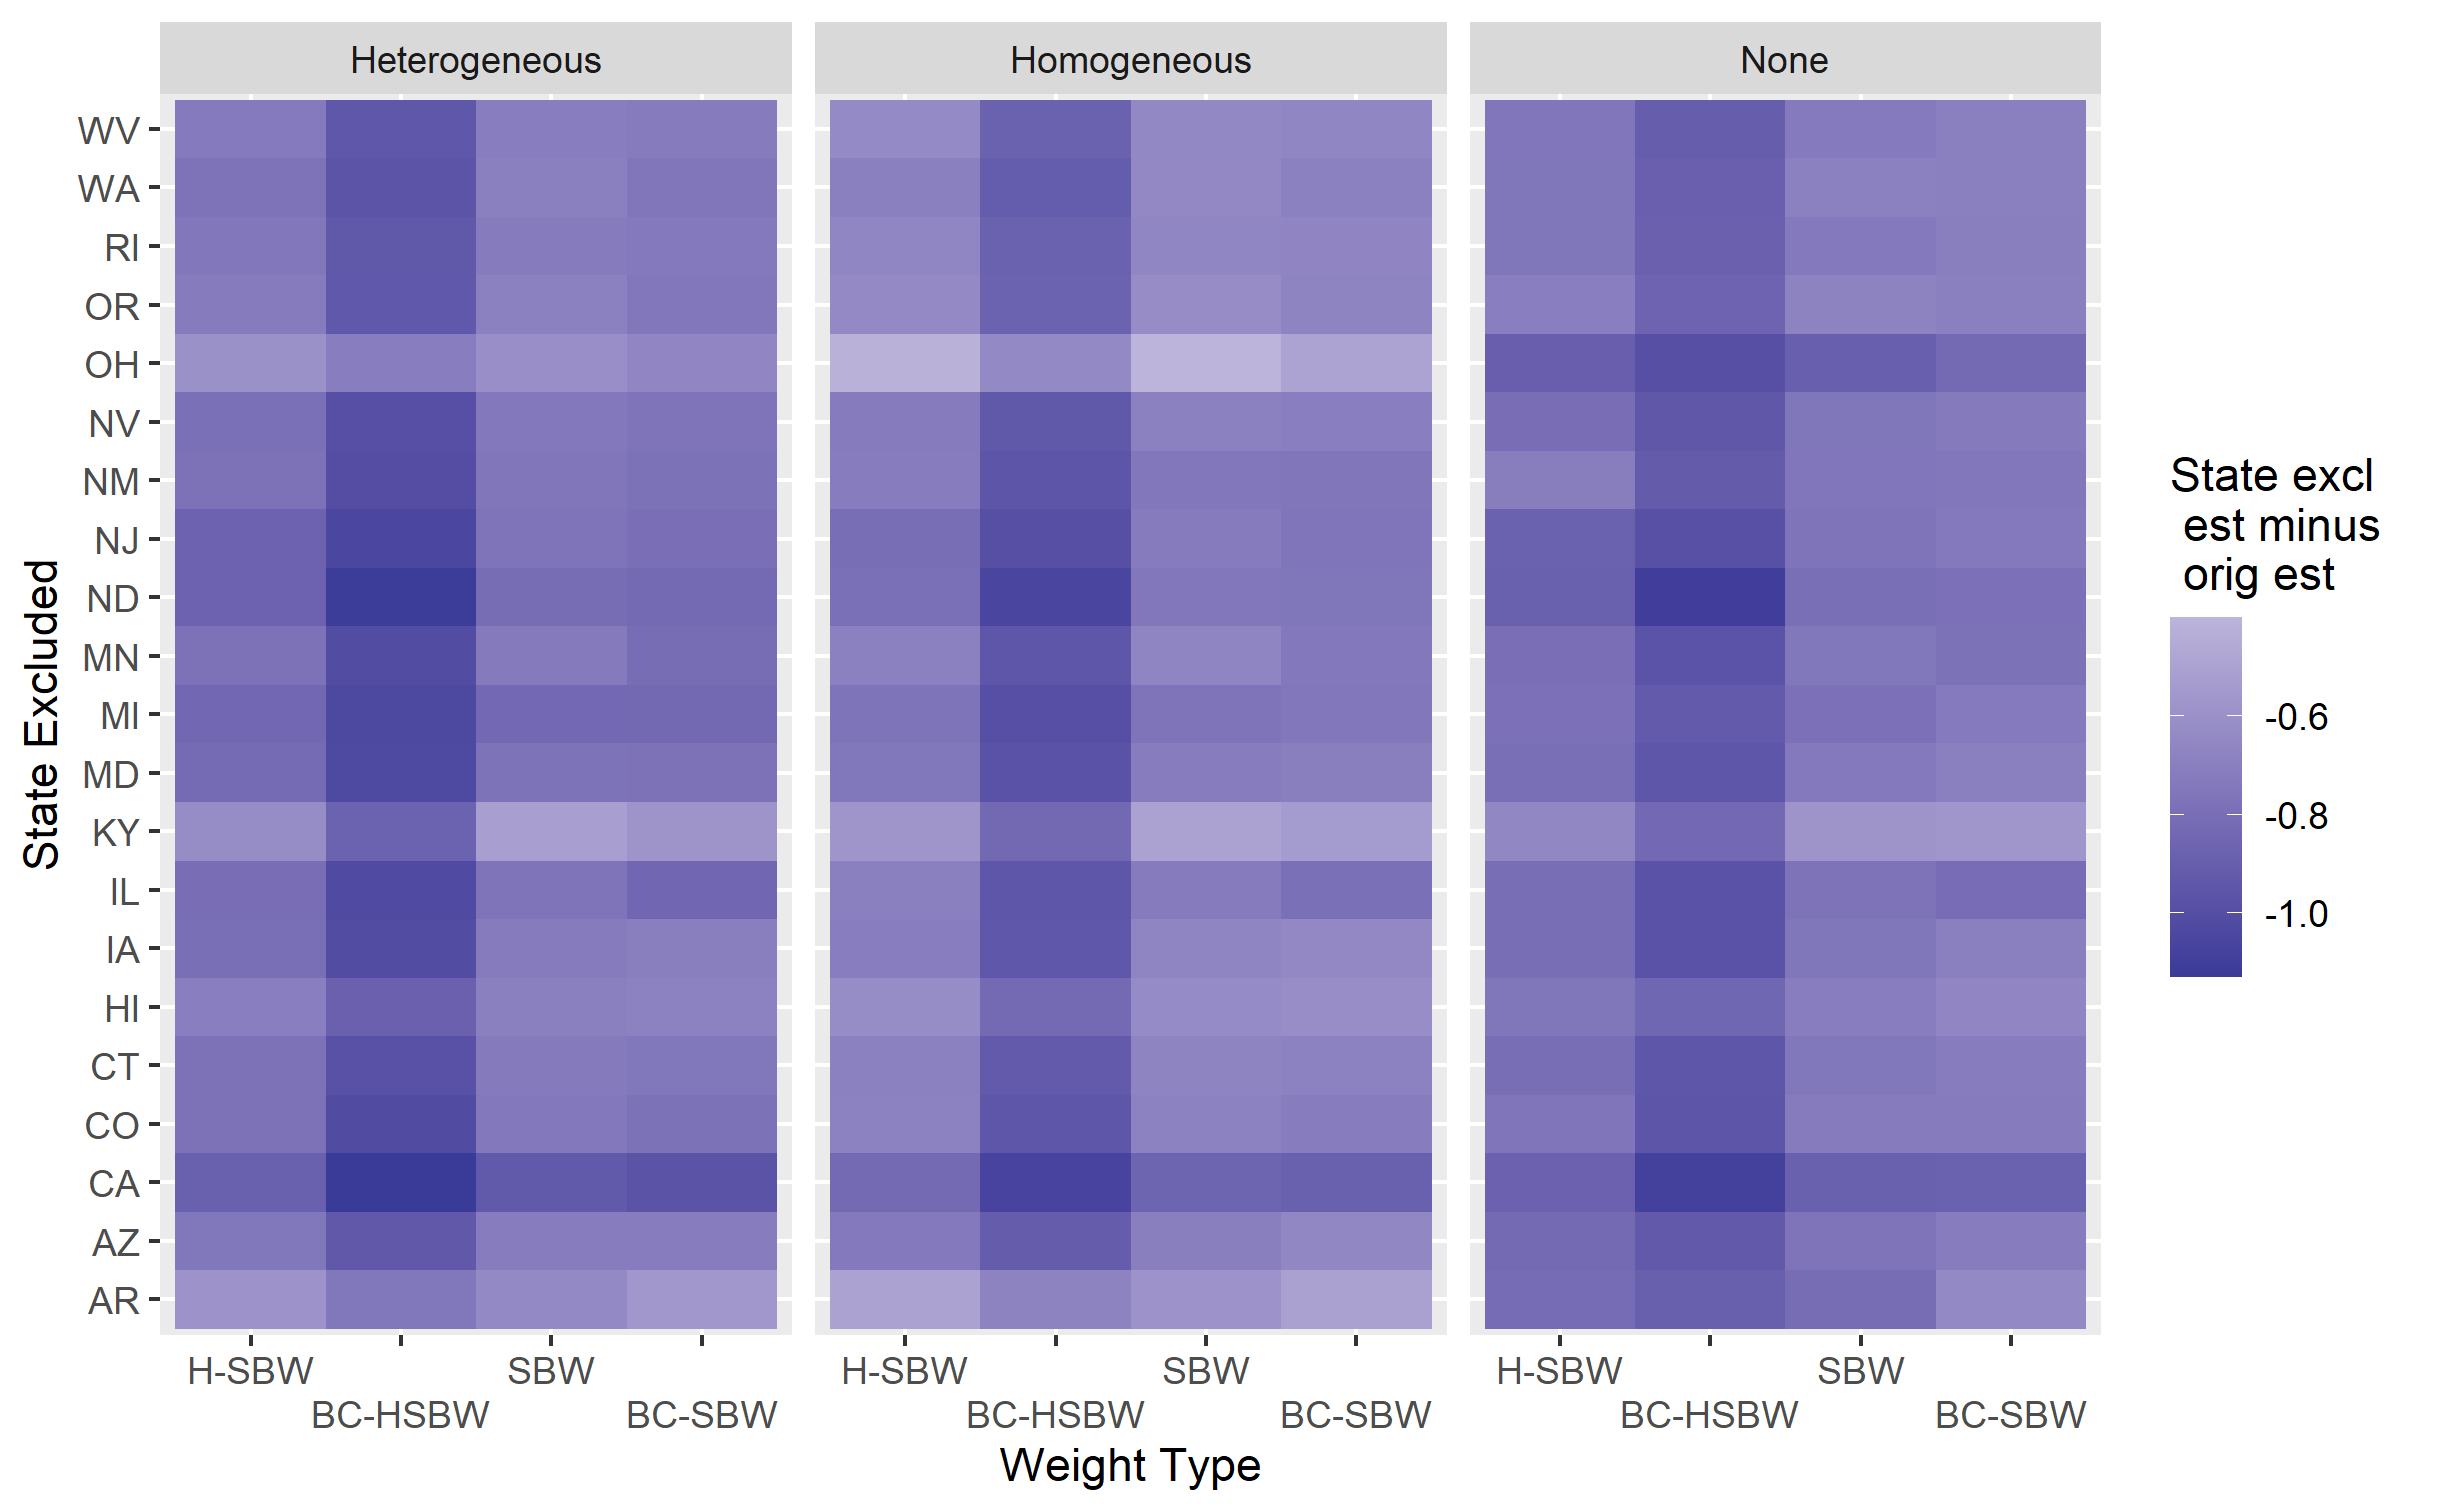
\includegraphics[scale=0.6]{01_Plots/loostate-repub-sensitivityc1-state-main.png}
    \caption{$\hat{\Delta}$ leave-one-out state, primary dataset, covariate adjustment constant}
    \label{fig:rdiffc1state}
\end{center}
\end{figure}

\begin{figure}[]
\begin{center}
    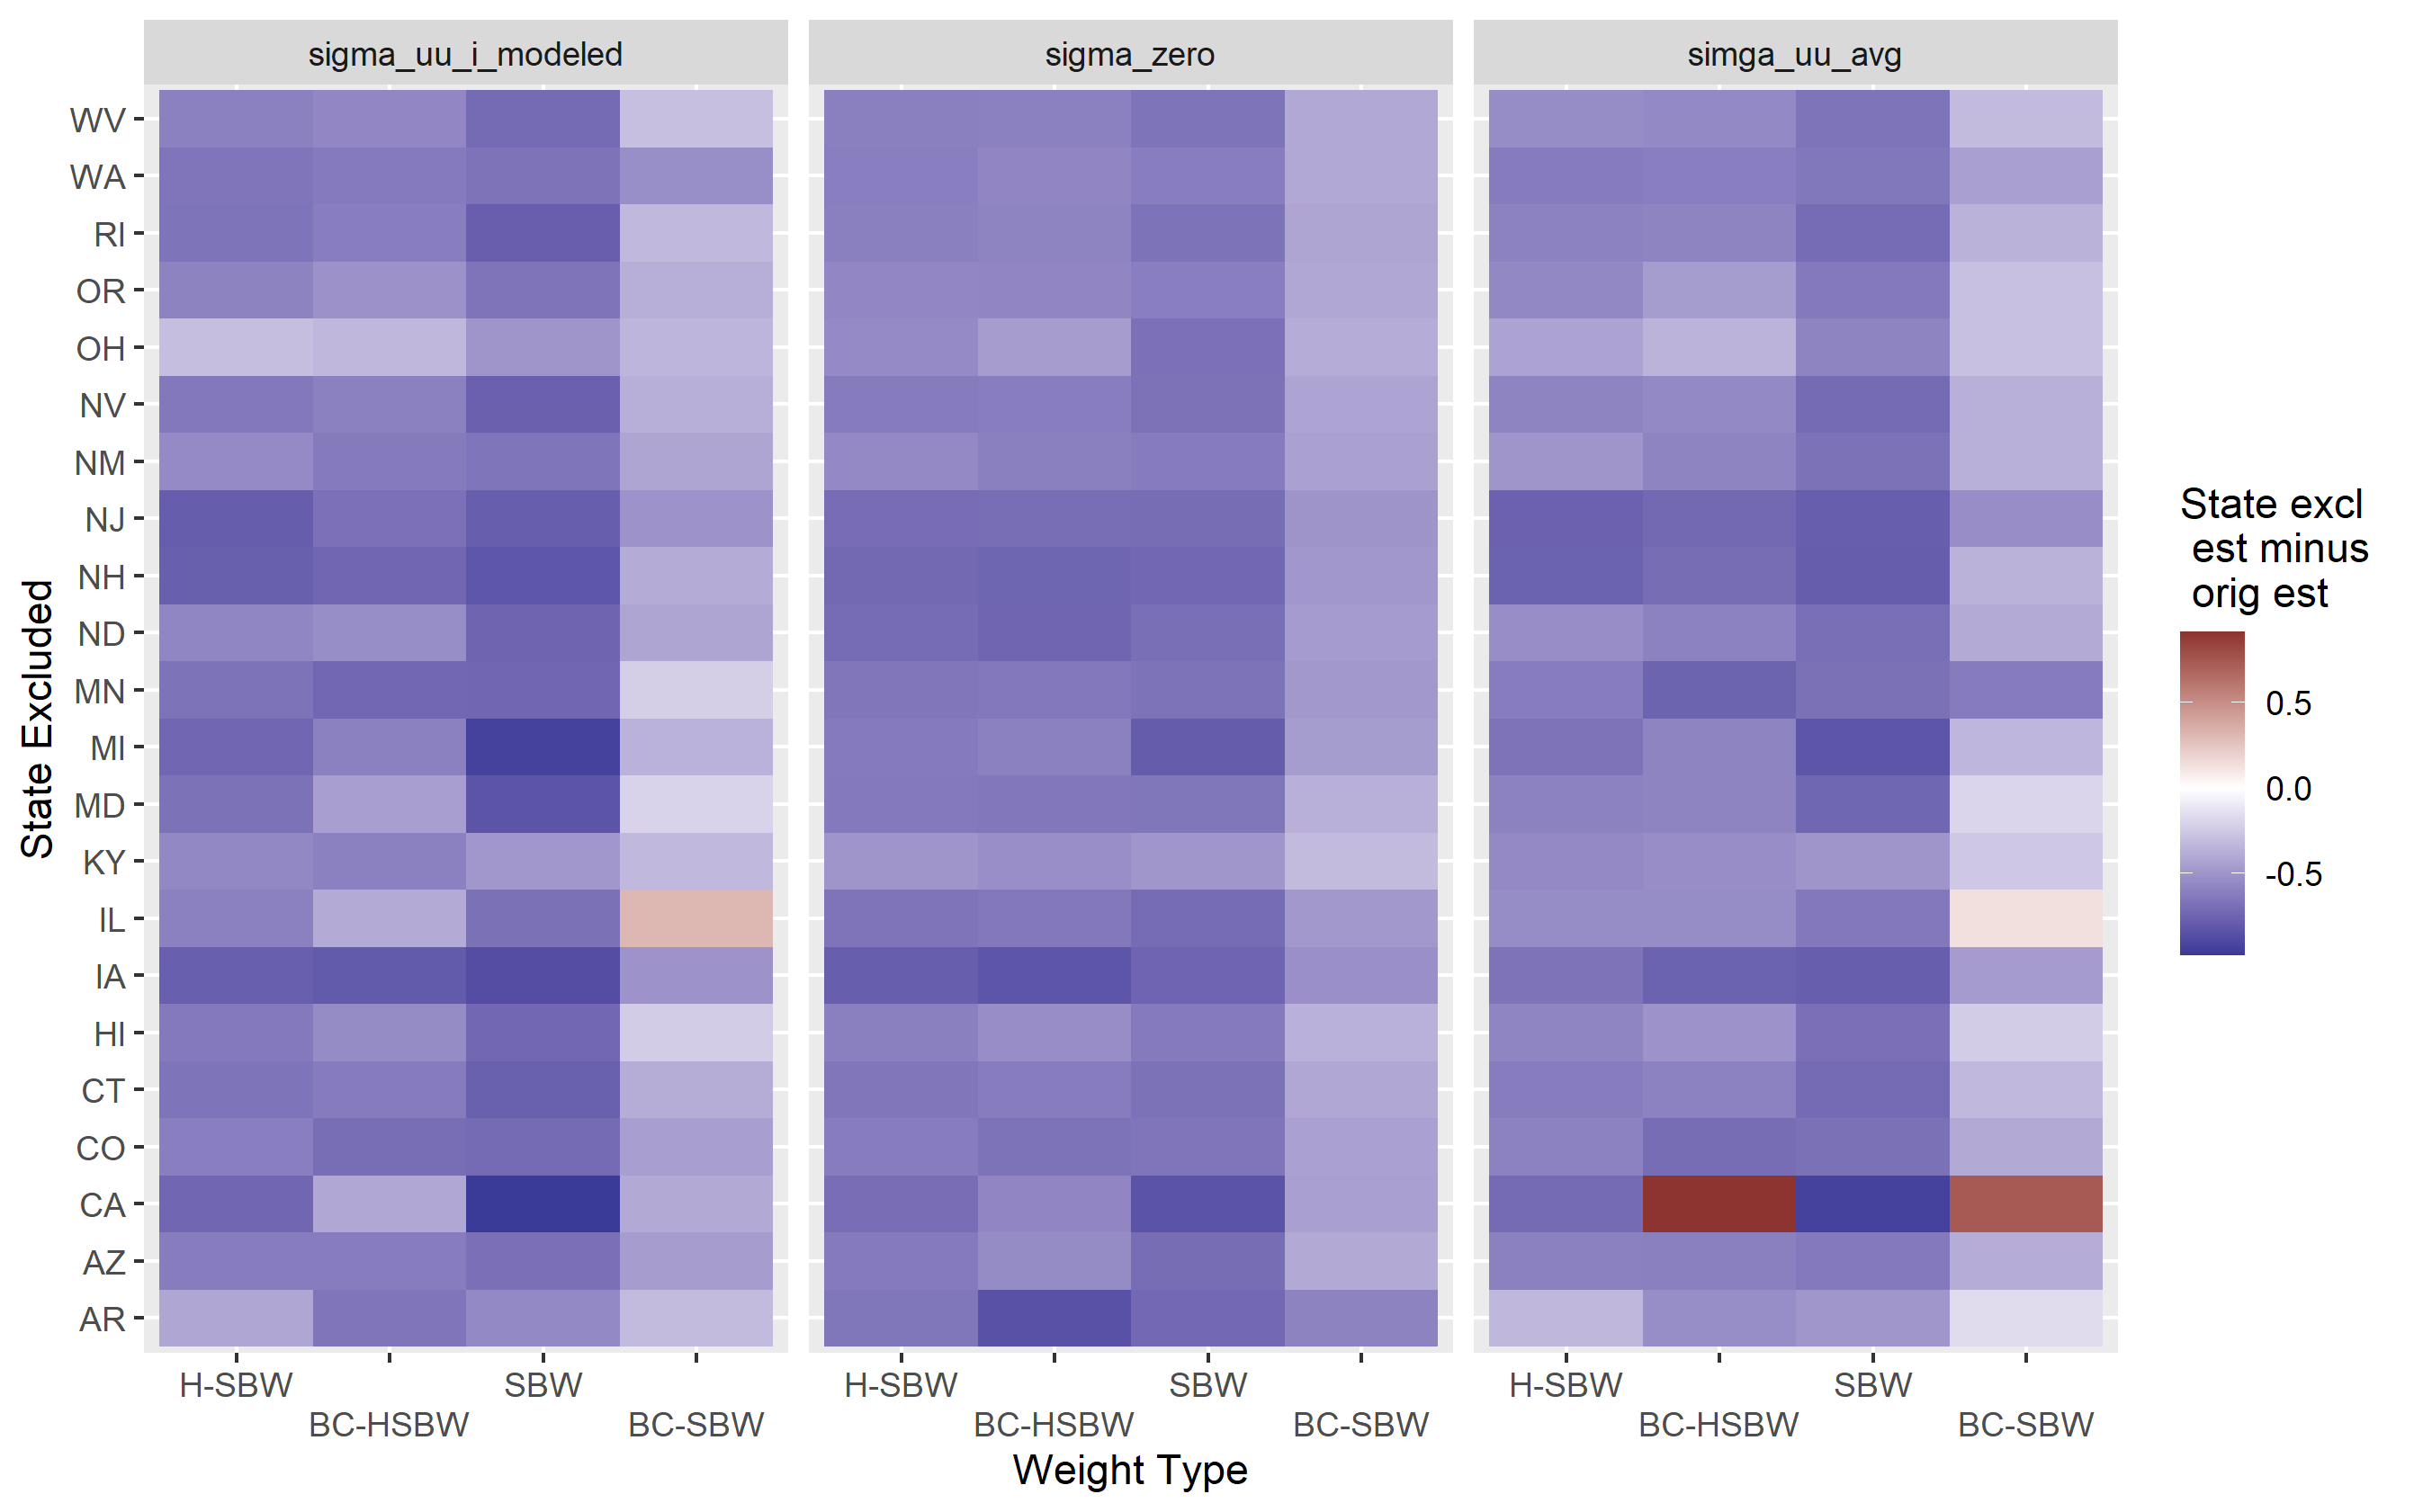
\includegraphics[scale=0.6]{01_Plots/loostate-repub-sensitivityc1-proc-main.png}
    \caption{$\hat{\Delta}$ leave-one-out state, primary dataset, covariate adjustment recalculated}
    \label{fig:rdiffc1proc}
\end{center}
\end{figure}

\begin{figure}[]
\begin{center}
    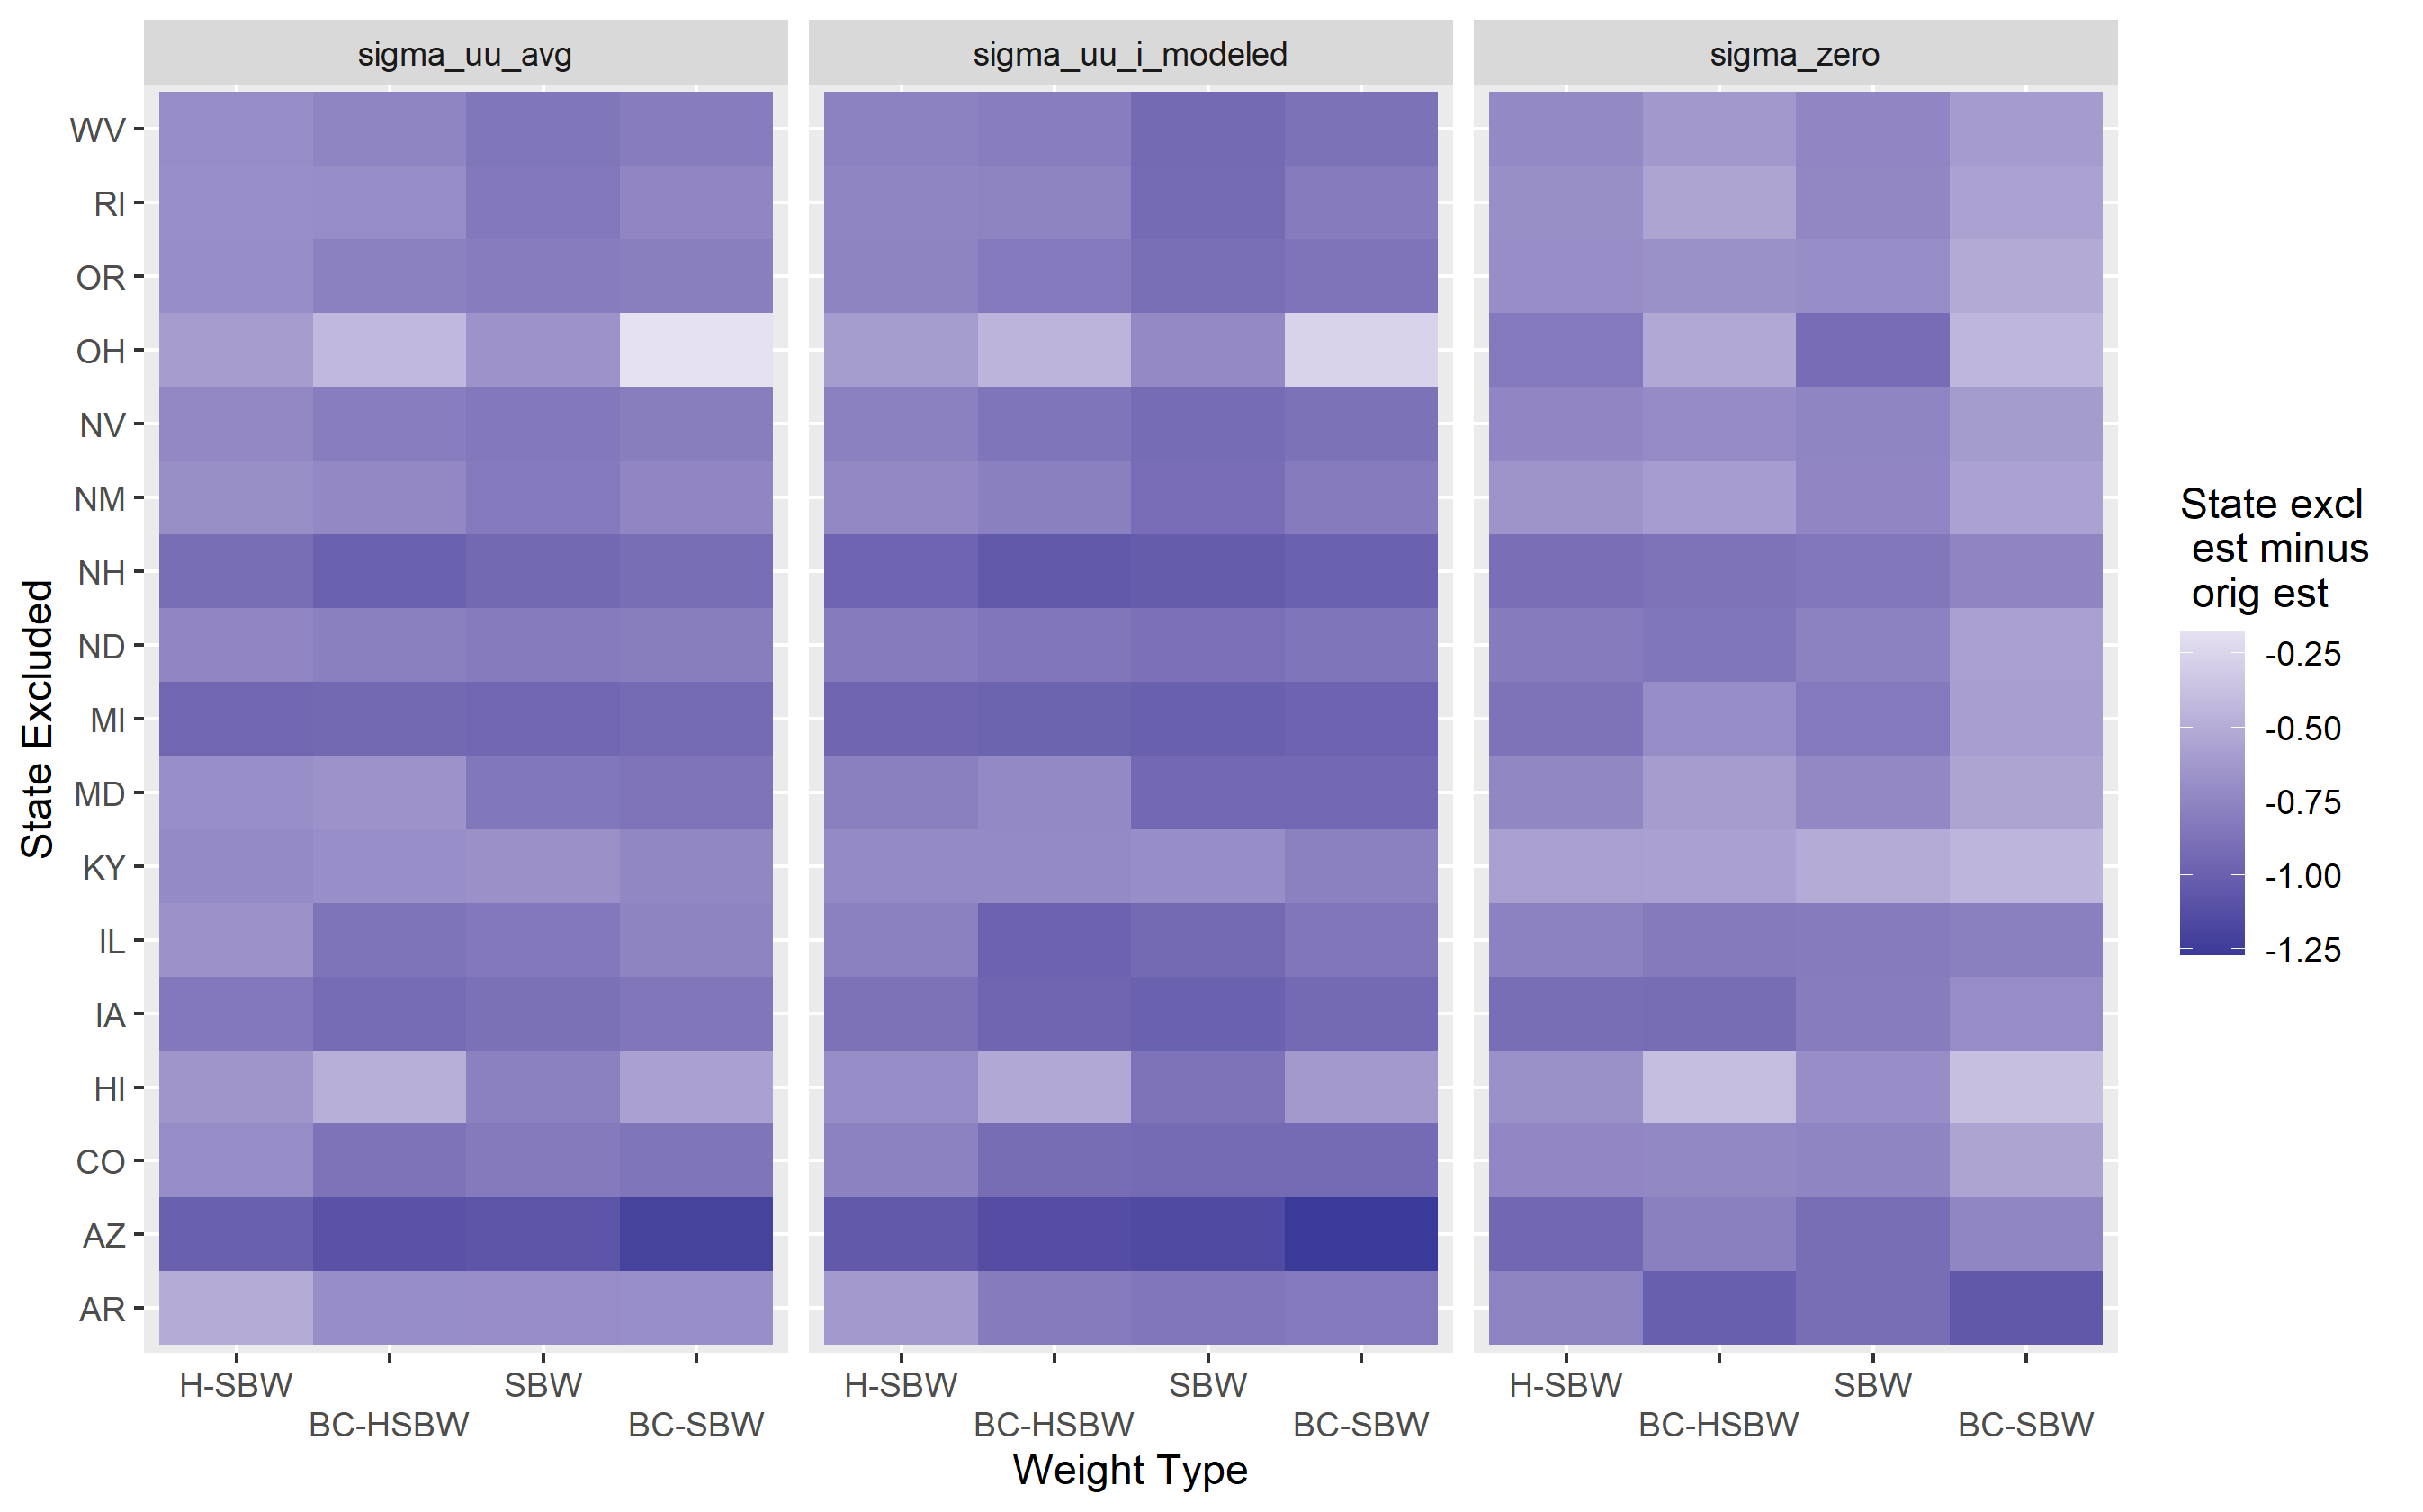
\includegraphics[scale=0.6]{01_Plots/loostate-repub-sensitivityc2-state-main.png}
    \caption{$\hat{\Delta}$ leave-one-out state, early expansion excluded, covariate adjustment constant}
    \label{fig:rdiffc2state}
\end{center}
\end{figure}

\begin{figure}[]
\begin{center}
    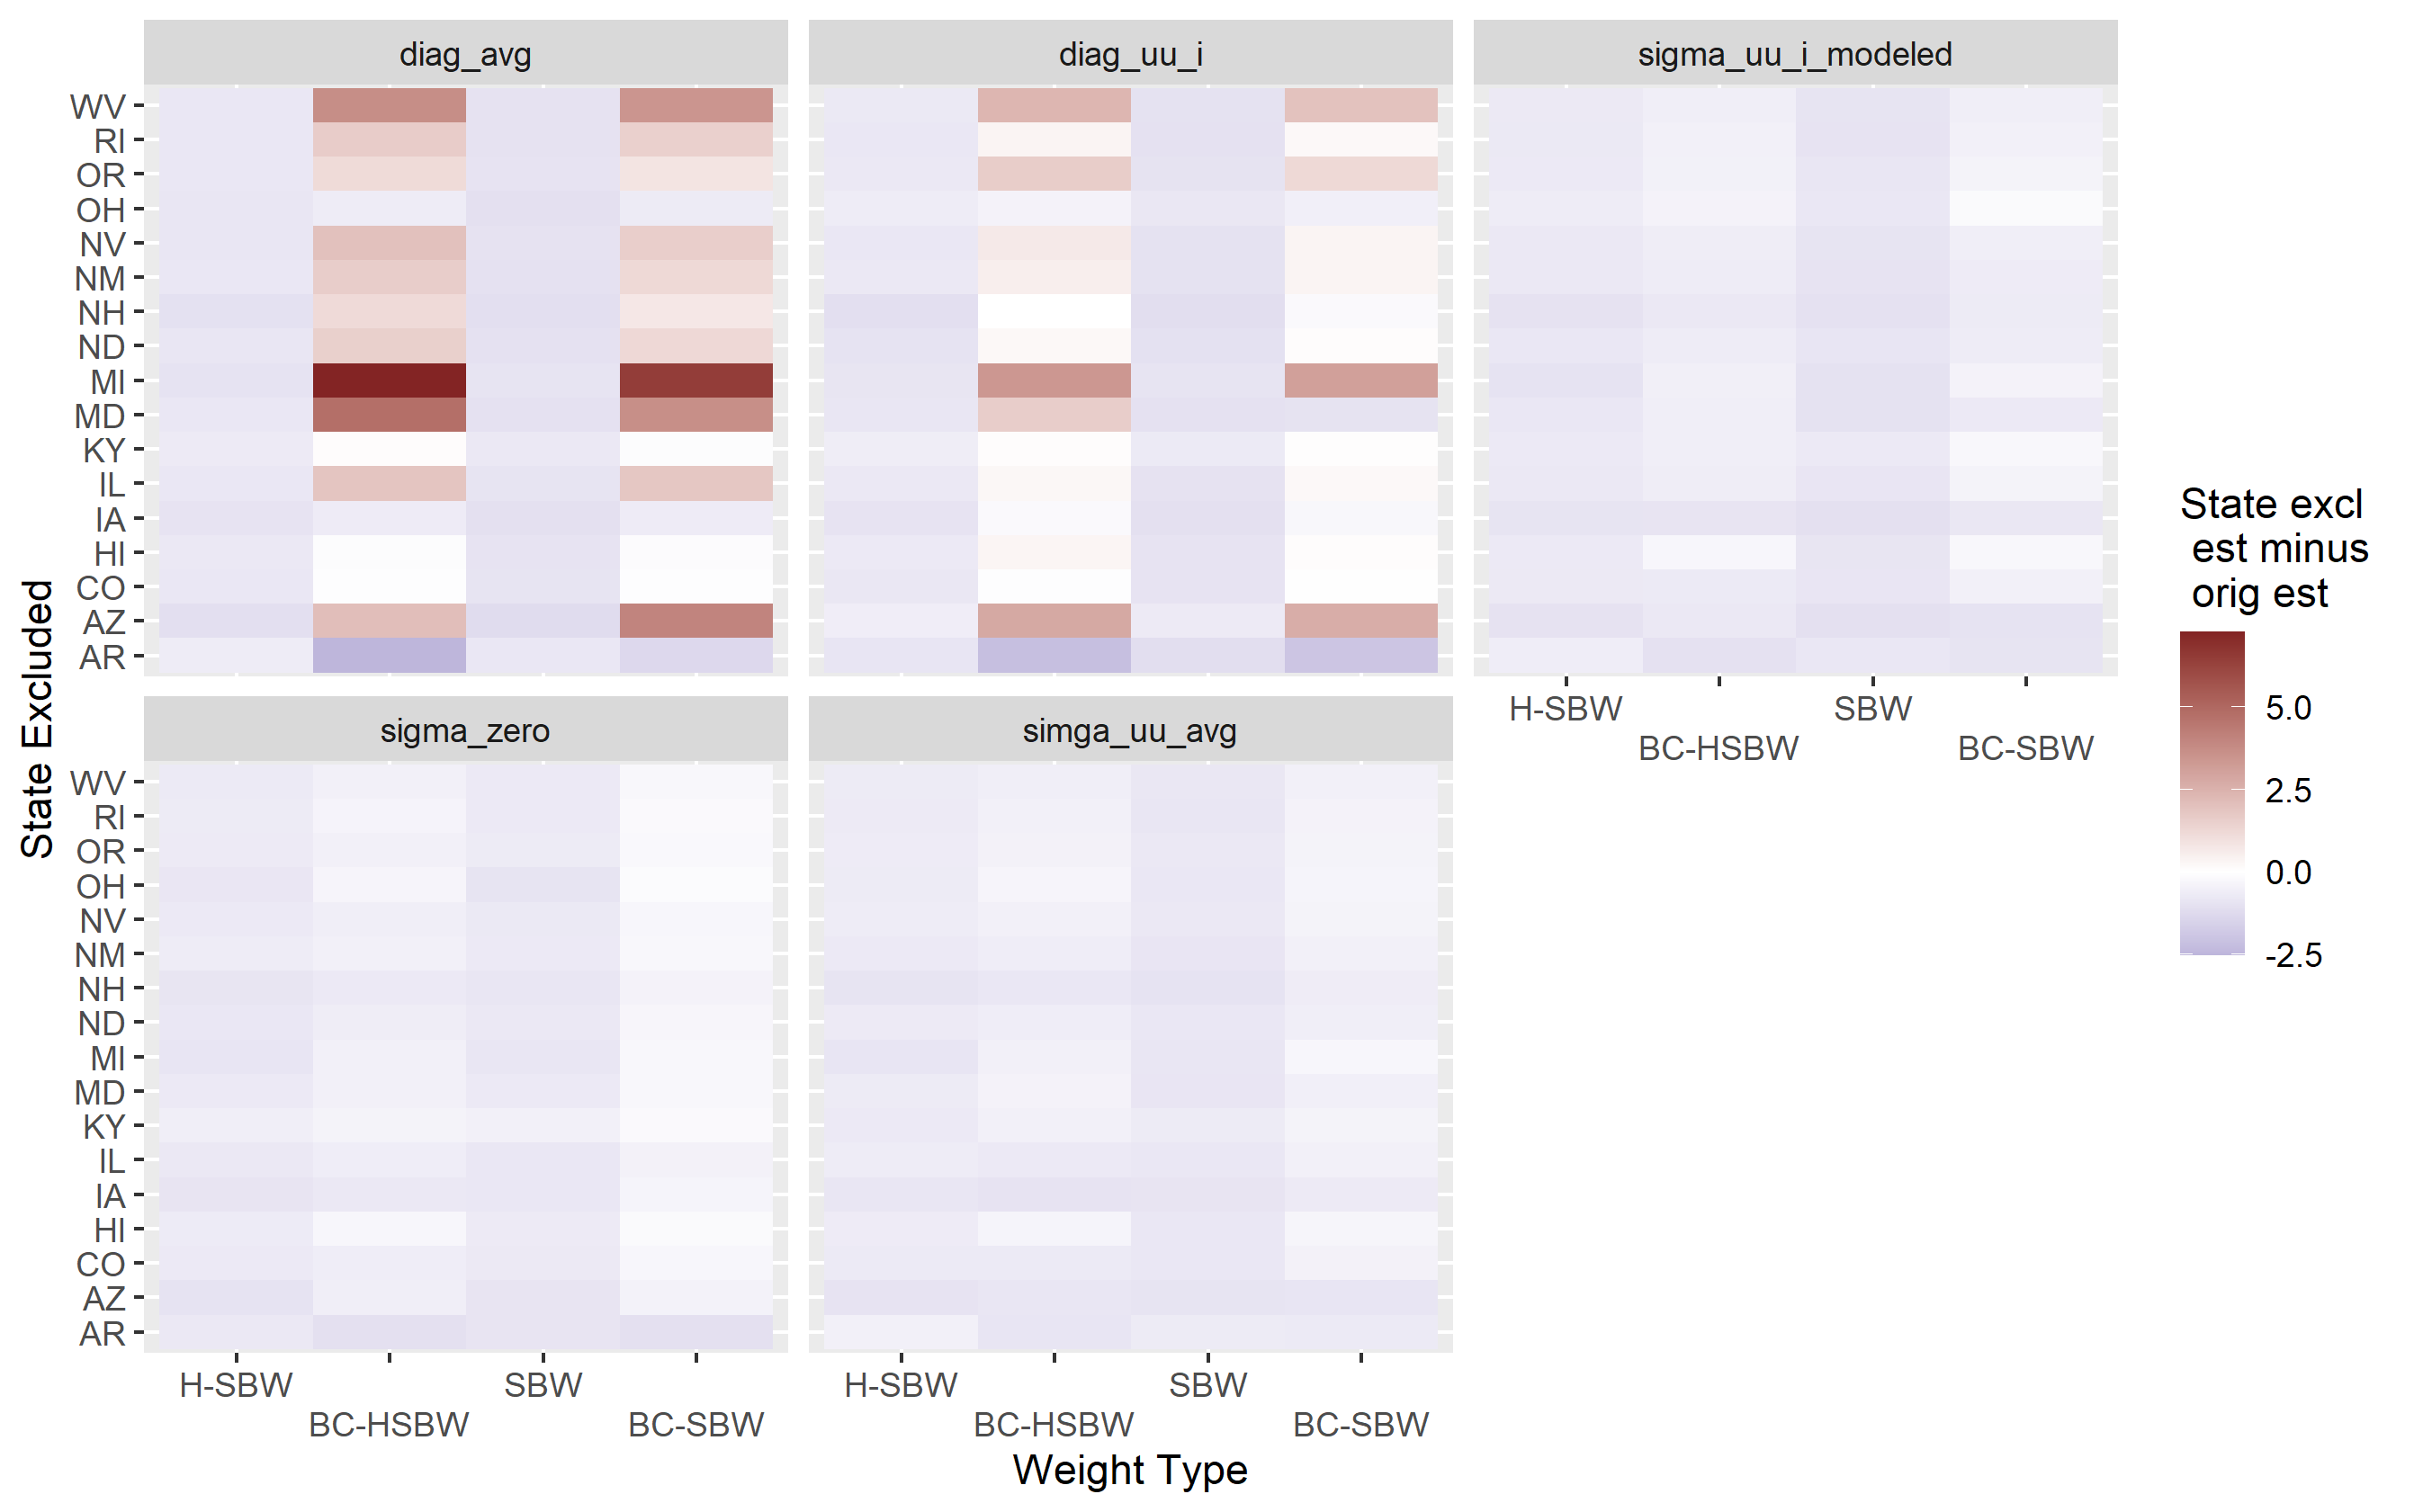
\includegraphics[scale=0.6]{01_Plots/loostate-repub-sensitivityc2-proc-main.png}
    \caption{$\hat{\Delta}$ leave-one-out state, early expansion excluded, covariate adjustment recalculated}
    \label{fig:rdiffc2proc}
\end{center}
\end{figure}

Table~\ref{tab:oateconfint} displays point estimates and confidence intervals for the primary point estimates for the OATE. We display the confidence intervals calculated using both the leave-one-out-states conditional on the covariate adjustment (CI (states)) and recalculating the covariate adjustment for the OATE (CI (proc)). We note that when calculating these confidence intervals, on the rare occasions when logistic regression failed to converge, we used the probit link instead.

\begin{table}[ht]
\centering
\begin{tabular}{rllll}
  \toprule
Psihat & Sigma estimate & Dataset & CI (states) & CI (proc) \\ 
  \midrule
-1.64 & sigma\_uu\_i & c1 & (-2.4, -0.89) & (-2.57, -0.72) \\ 
  -1.58 & sigma\_avg & c1 & (-2.17, -1) & (-2.37, -0.79) \\ 
  -1.80 & sigma\_zero & c1 & (-2.49, -1.1) & (-2.49, -1.1) \\ 
  -1.81 & sigma\_uu\_i & c2 & (-2.47, -1.15) & (-2.63, -0.98) \\ 
  -1.74 & sigma\_avg & c2 & (-2.28, -1.2) & (-2.44, -1.04) \\ 
  -1.95 & sigma\_zero & c2 & (-2.65, -1.25) & (-2.65, -1.25) \\ 
   \bottomrule
\end{tabular}
\caption{OATE primary results inference}
\label{tab:oateconfint}
\end{table}

Table~\ref{tab:oaterepubdiff} displays the difference between the estimated contrasts when excluding Republican governance indicators and when including all covariates as well as the estimated confidence intervals, estimated both conditional on the imputation (CI (states)) and recalculating the entire covariate adjustment (CI (proc)).

\begin{table}[ht]
\centering
\begin{tabular}{llrll}
  \toprule
Sigma estimate & Dataset & $\hat{\Delta}$ & CI (states) & CI (proc) \\ 
  \midrule
sigma\_uu\_i & c1 & -0.96 & (-1.1, -0.81) & (-1.12, -0.8) \\ 
  sigma\_uu\_i & c2 & -0.72 & (-0.87, -0.57) & (-0.89, -0.55) \\ 
  sigma\_avg & c1 & -1.04 & (-1.19, -0.89) & (-1.22, -0.86) \\ 
  sigma\_avg & c2 & -0.80 & (-0.98, -0.63) & (-0.99, -0.61) \\ 
  sigma\_zero & c1 & -0.75 & (-0.88, -0.63) & (-0.88, -0.63) \\ 
  sigma\_zero & c2 & -0.56 & (-0.69, -0.43) & (-0.69, -0.43) \\ 
   \bottomrule
\end{tabular}
\caption{OATE $\hat{\Delta}$ estimates}
\label{tab:oaterepubdiff}
\end{table}

Table~\ref{tab:oatesensitive} presents all point estimates calculate using the overlap weights. Dataset ``c1'' refers to the primary dataset and dataset ``c2'' removes the early expansion states. The numeric column names refer to the covariate group excluded (covariate groups described above).

\begin{table}[ht]
\centering
\begin{tabular}{llrrrrrr}
  \toprule
Sigma estimate & Dataset & 0 & 1 & 2 & 3 & 4 & 5 \\ 
  \midrule
sigma\_uu\_i & c1 & -1.64 & -2.60 & -2.96 & -1.86 & -1.86 & -1.77 \\ 
  sigma\_uu\_i & c2 & -1.81 & -2.53 & -3.10 & -2.18 & -2.04 & -1.96 \\ 
  sigma\_avg & c1 & -1.58 & -2.62 & -2.85 & -1.76 & -1.76 & -1.78 \\ 
  sigma\_avg & c2 & -1.74 & -2.54 & -3.00 & -2.10 & -1.96 & -1.95 \\ 
  sigma\_zero & c1 & -1.80 & -2.55 & -3.11 & -1.98 & -1.94 & -1.83 \\ 
  sigma\_zero & c2 & -1.95 & -2.51 & -3.25 & -2.12 & -2.10 & -2.00 \\ 
   \bottomrule
\end{tabular}
\caption{OATE all point estimates}
\label{tab:oatesensitive}
\end{table}

Figure~\ref{fig:oateheatmap} displays a heatmap showing how the OATE point estimates change when removing each state, conditional on our preferred covariate adjustment for both the primary dataset and when excluding early expansion states. We present the results for all covariates and excluding the Republican governance indicators. Additional results are available on request. We see that our point estimates move closer to zero when removing Wisconsin or Ohio for all specifications. Removing Arkansas appears to generally move the point estimates further away from zero.

\begin{figure}[]
\begin{center}
    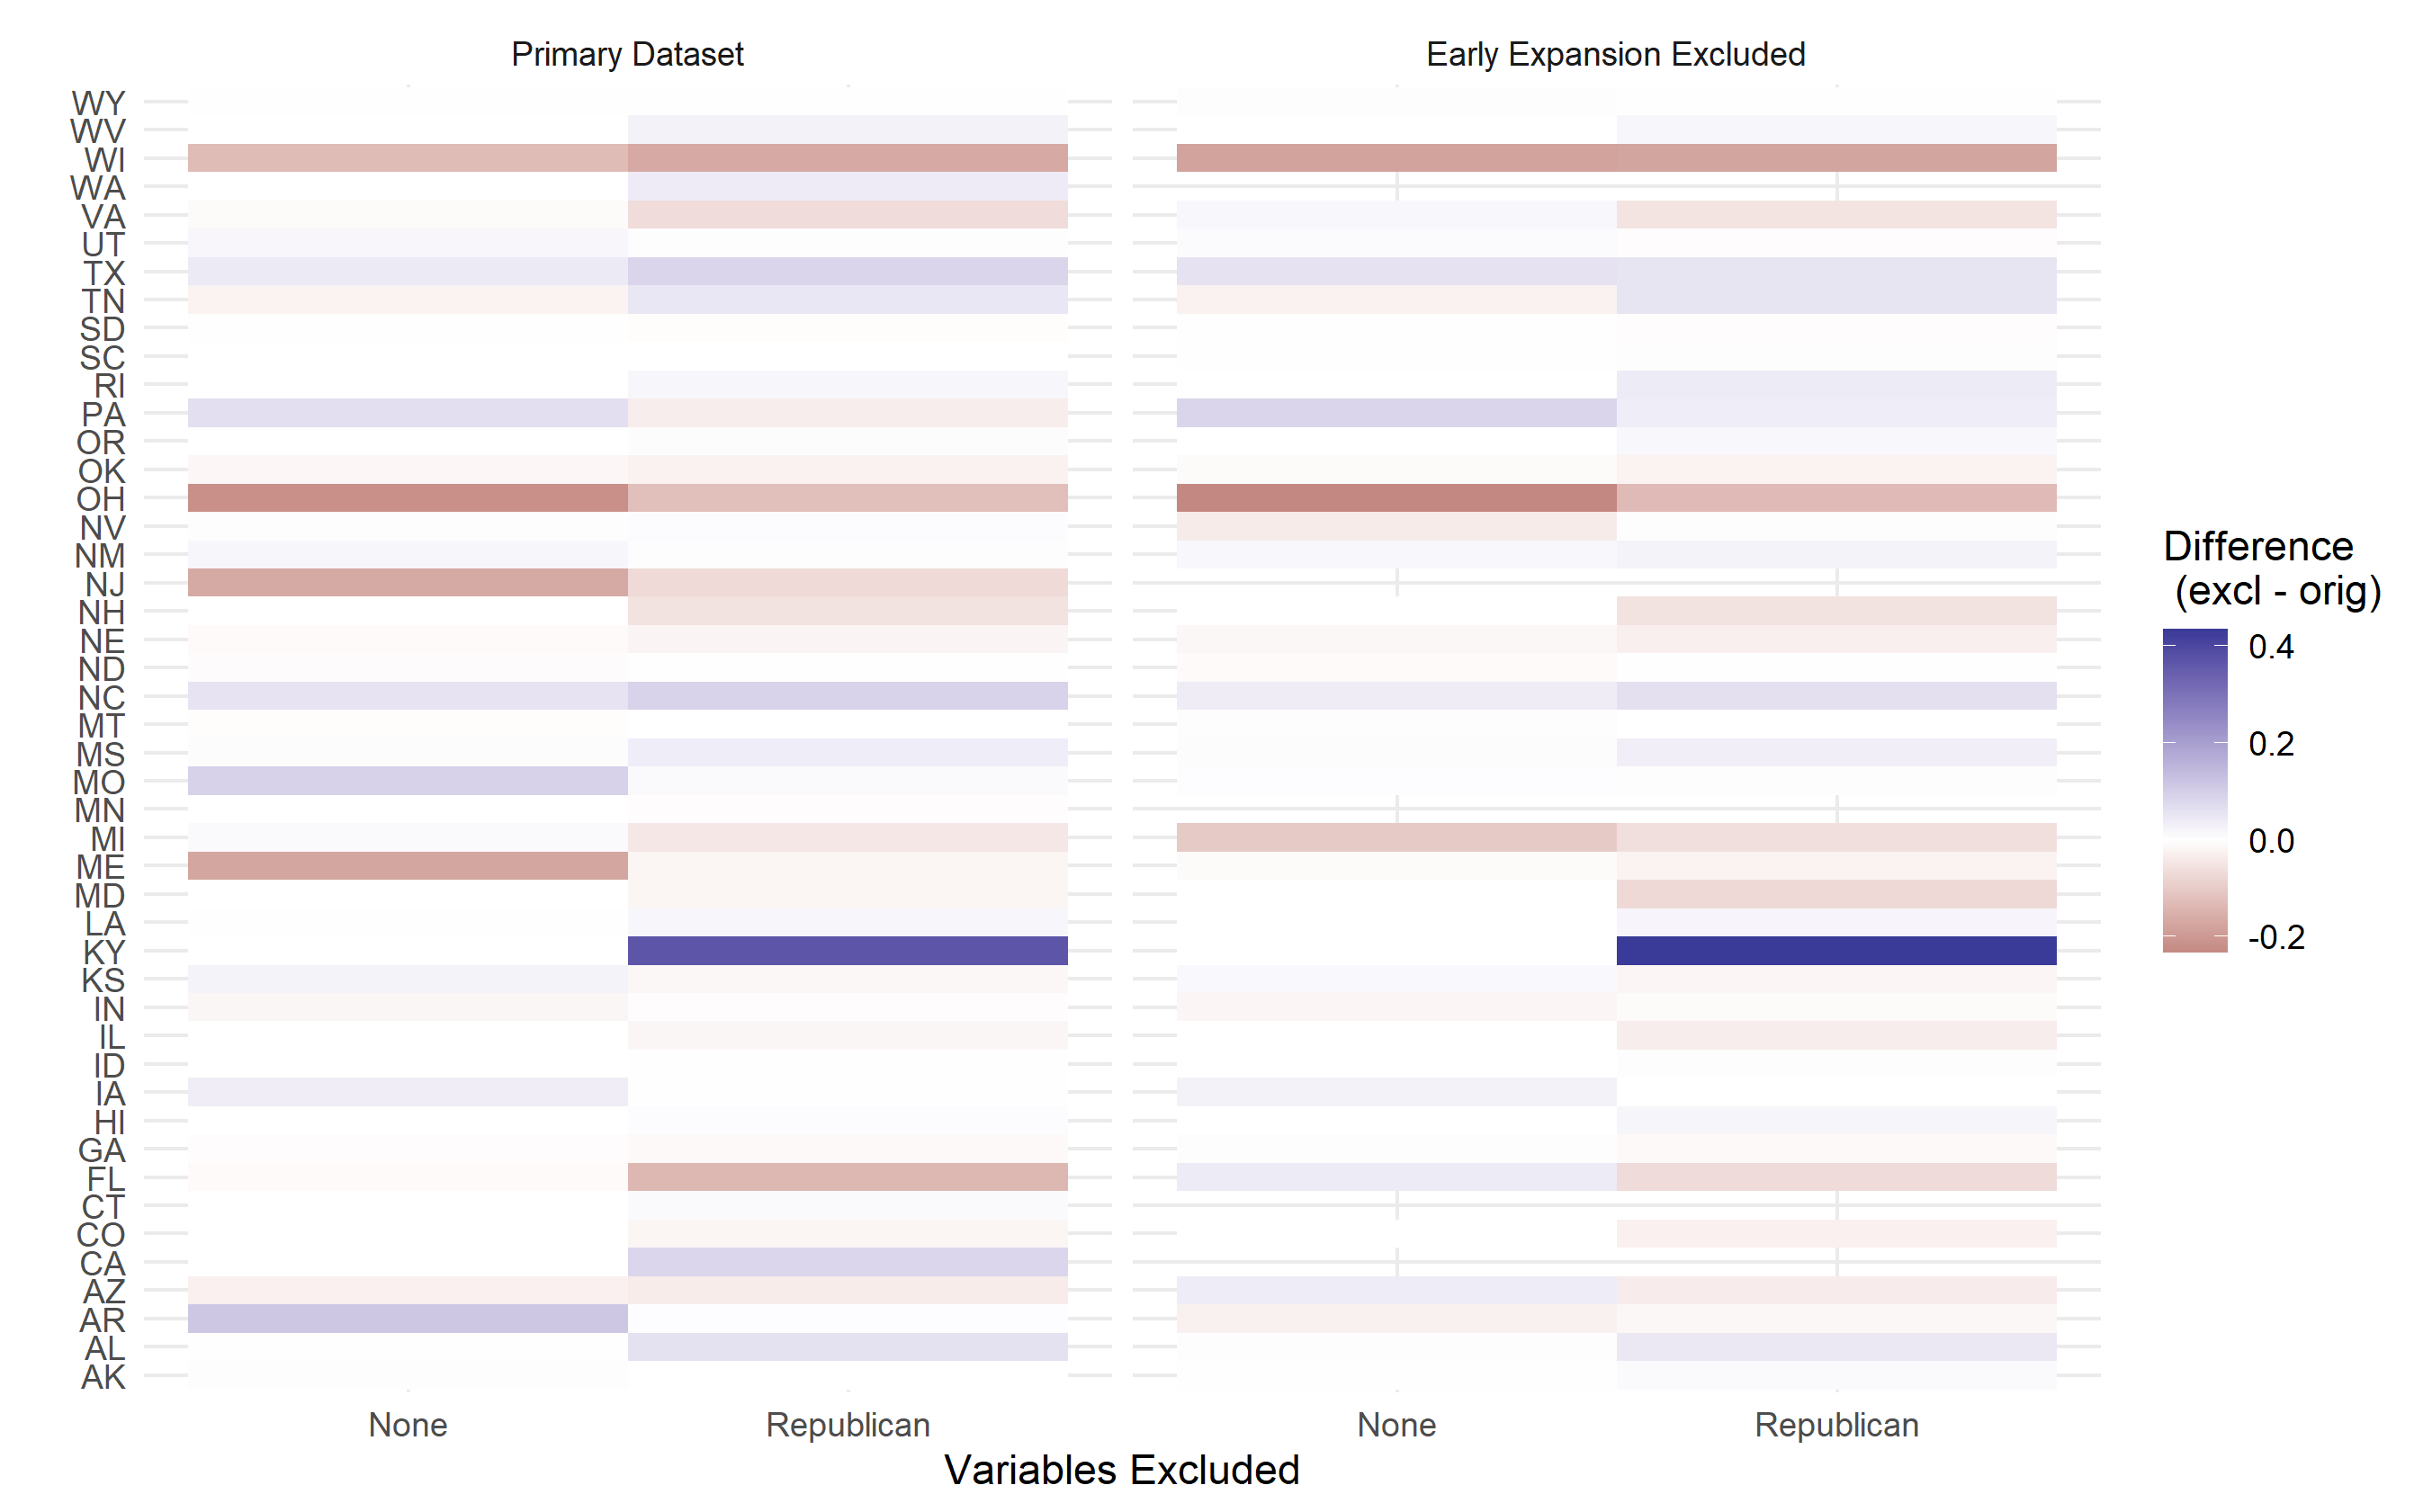
\includegraphics[scale=0.6]{01_Plots/oate-loo-state-cov-group-heatmap-states.png}
    \caption{OATE estimates, leave-one-out-states analysis}
    \label{fig:oateheatmap}
\end{center}
\end{figure}

\end{document}






